% Лабораторная работа по РЗП № 1
% Михедов Константин Константинович

% Тип документа: статья, на бумаге А4
\documentclass[a4paper]{article}

% Подключение сторонних tex файлов 
\usepackage{import}


% Основные данные - ВУЗ, факультет, город...
\import{./../../../stuff/tex}{config.tex}

% Подключение необходимых зависимостей
\import{./../../../stuff/tex/settings}{packages.tex}
% Настройка подключенных пакетов
\import{./../../../stuff/tex/settings}{preferences.tex}


% Шаблон титульной страницы 
\import{./../../../stuff/tex/templates}{title.tex}
% Упрощенный блок "выполнил"
\import{./../../../stuff/tex/templates}{sign1.tex}
% Макрос для содержания
\import{./../../../stuff/tex/templates}{toc.tex}

% Определяем название документа
\title{
  Лабораторная работа №1 по курсу \\
  <<Разработка защищенных приложений>>  
}
% Отключаем отображение правительства
\renewcommand{\government}{}
% Отключаем сокращенное нзавание университета
\renewcommand{\subuniversity}{}
% Указываем преподавателя
\renewcommand{\shortteachername}{Башун В.В.}


% Путь до внешних изображений
\graphicspath{ {./../figures/}}


% Основной текст работы
\begin{document}
  \templatedtitlepage
  
  \toc
  \section{Ход работы}

  \subsection{Создание репозитория}

  \begin{figure}[H]
    \centering
    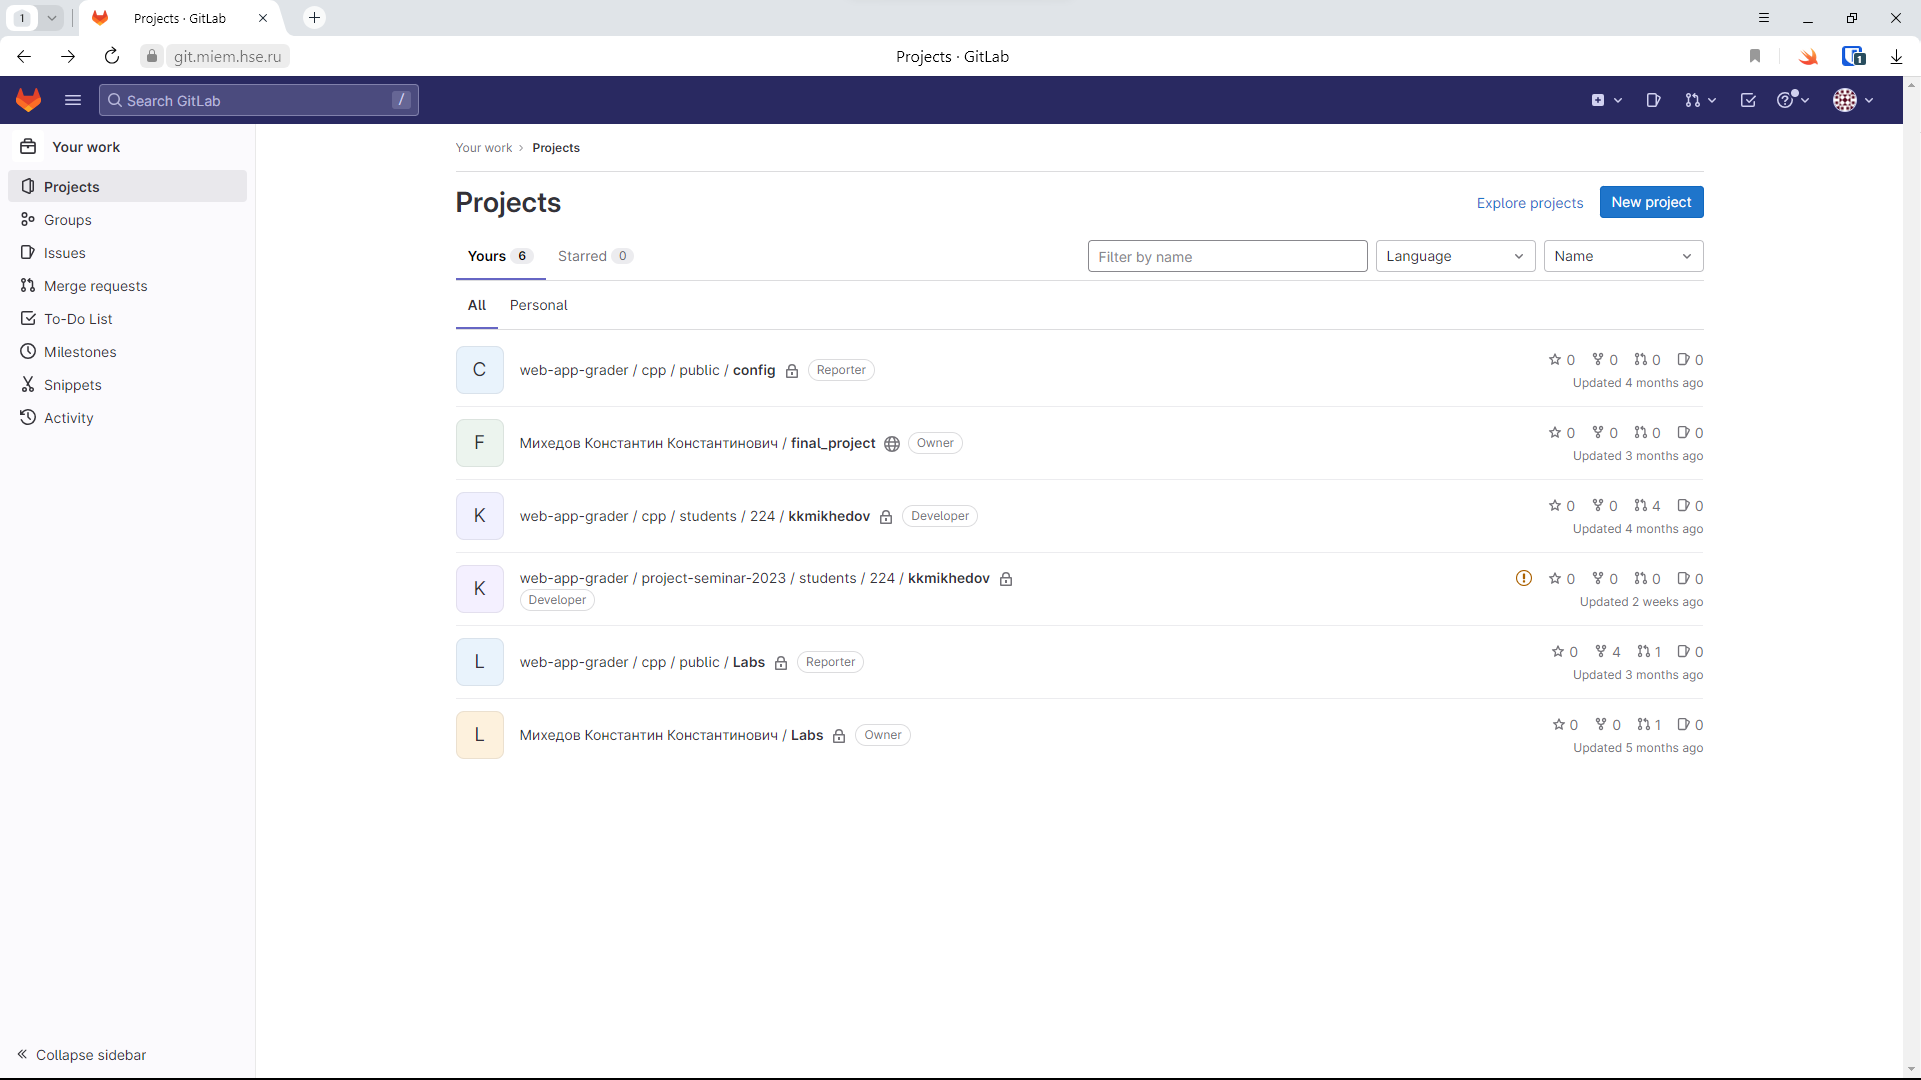
\includegraphics[width=\textwidth]{1_ (60)}
    \caption{Открываем GitLab, нажимаем на кнопку <<New Project>>}
  \end{figure}

  \begin{figure}[H]
    \centering
    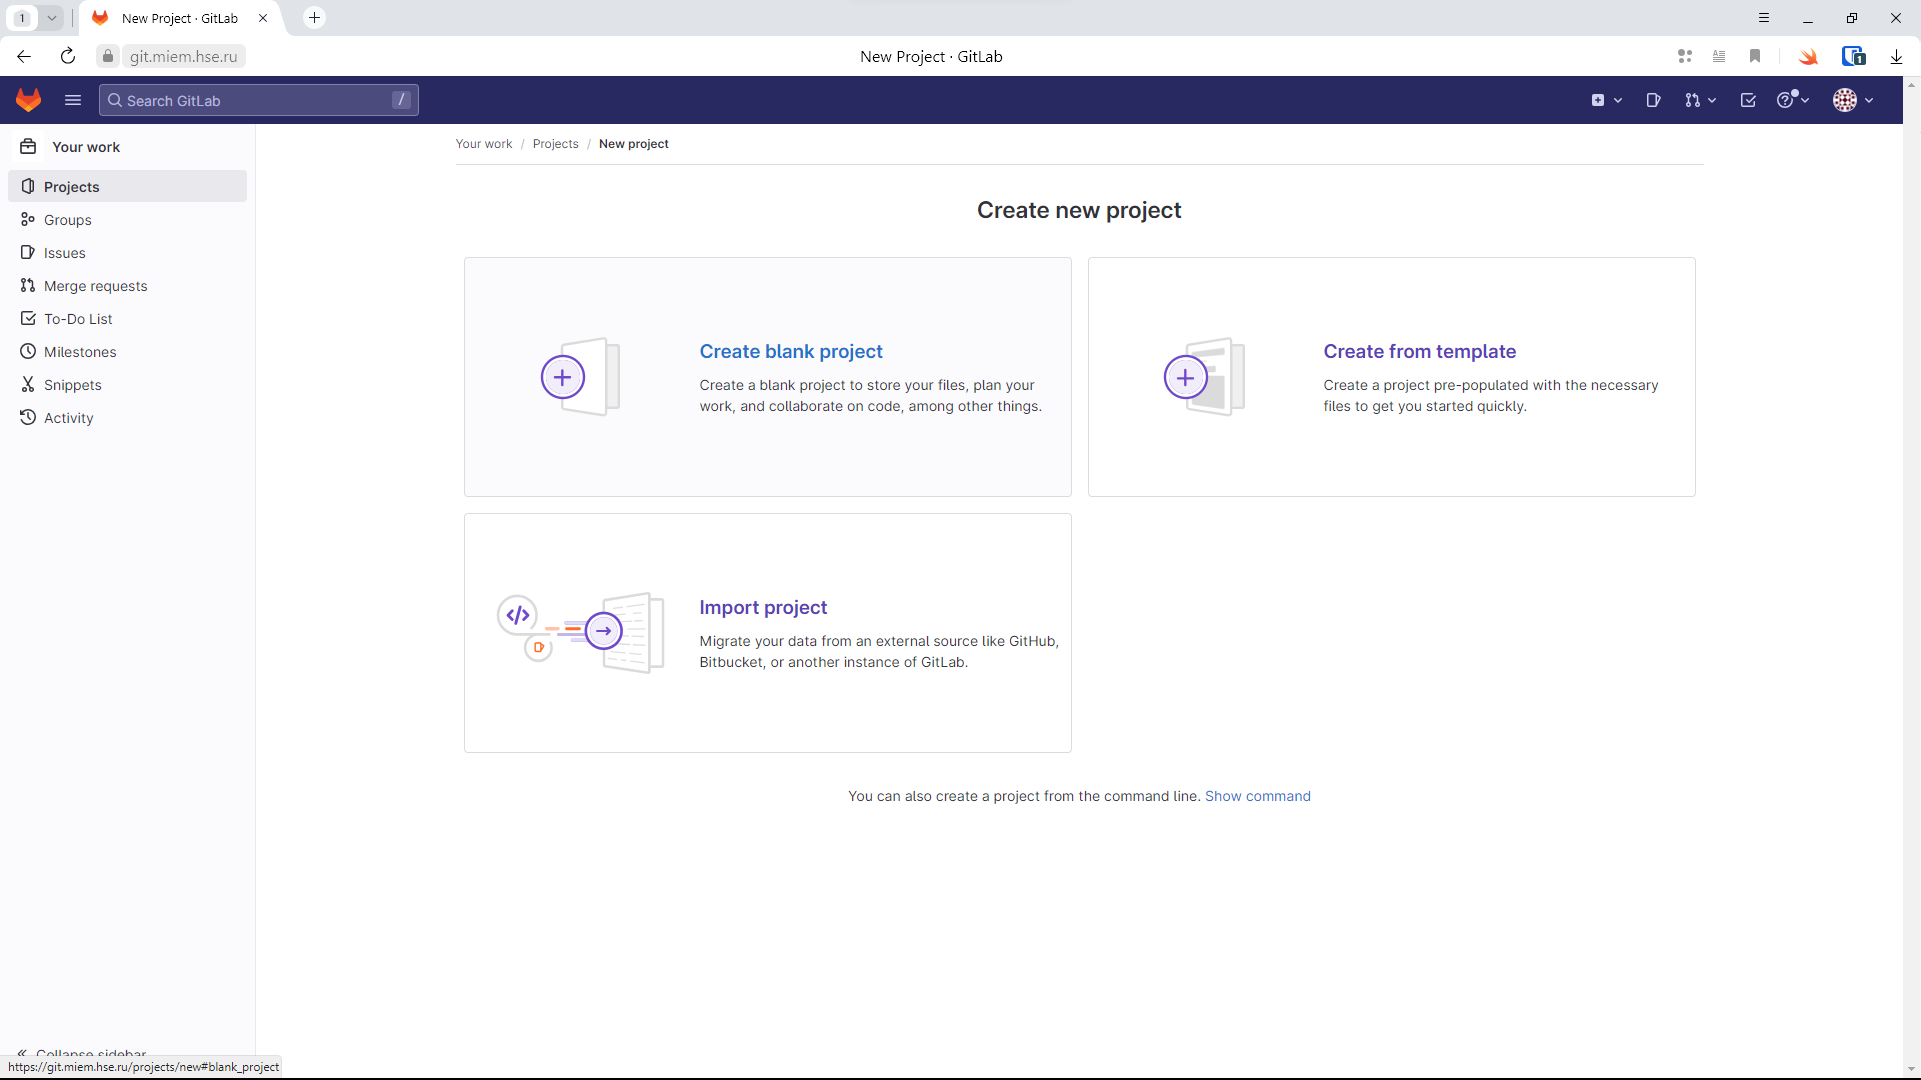
\includegraphics[width=\textwidth]{1_ (59)}
    \caption{Выбираем тип <<blank project>>}
  \end{figure}

  \begin{figure}[H]
    \centering
    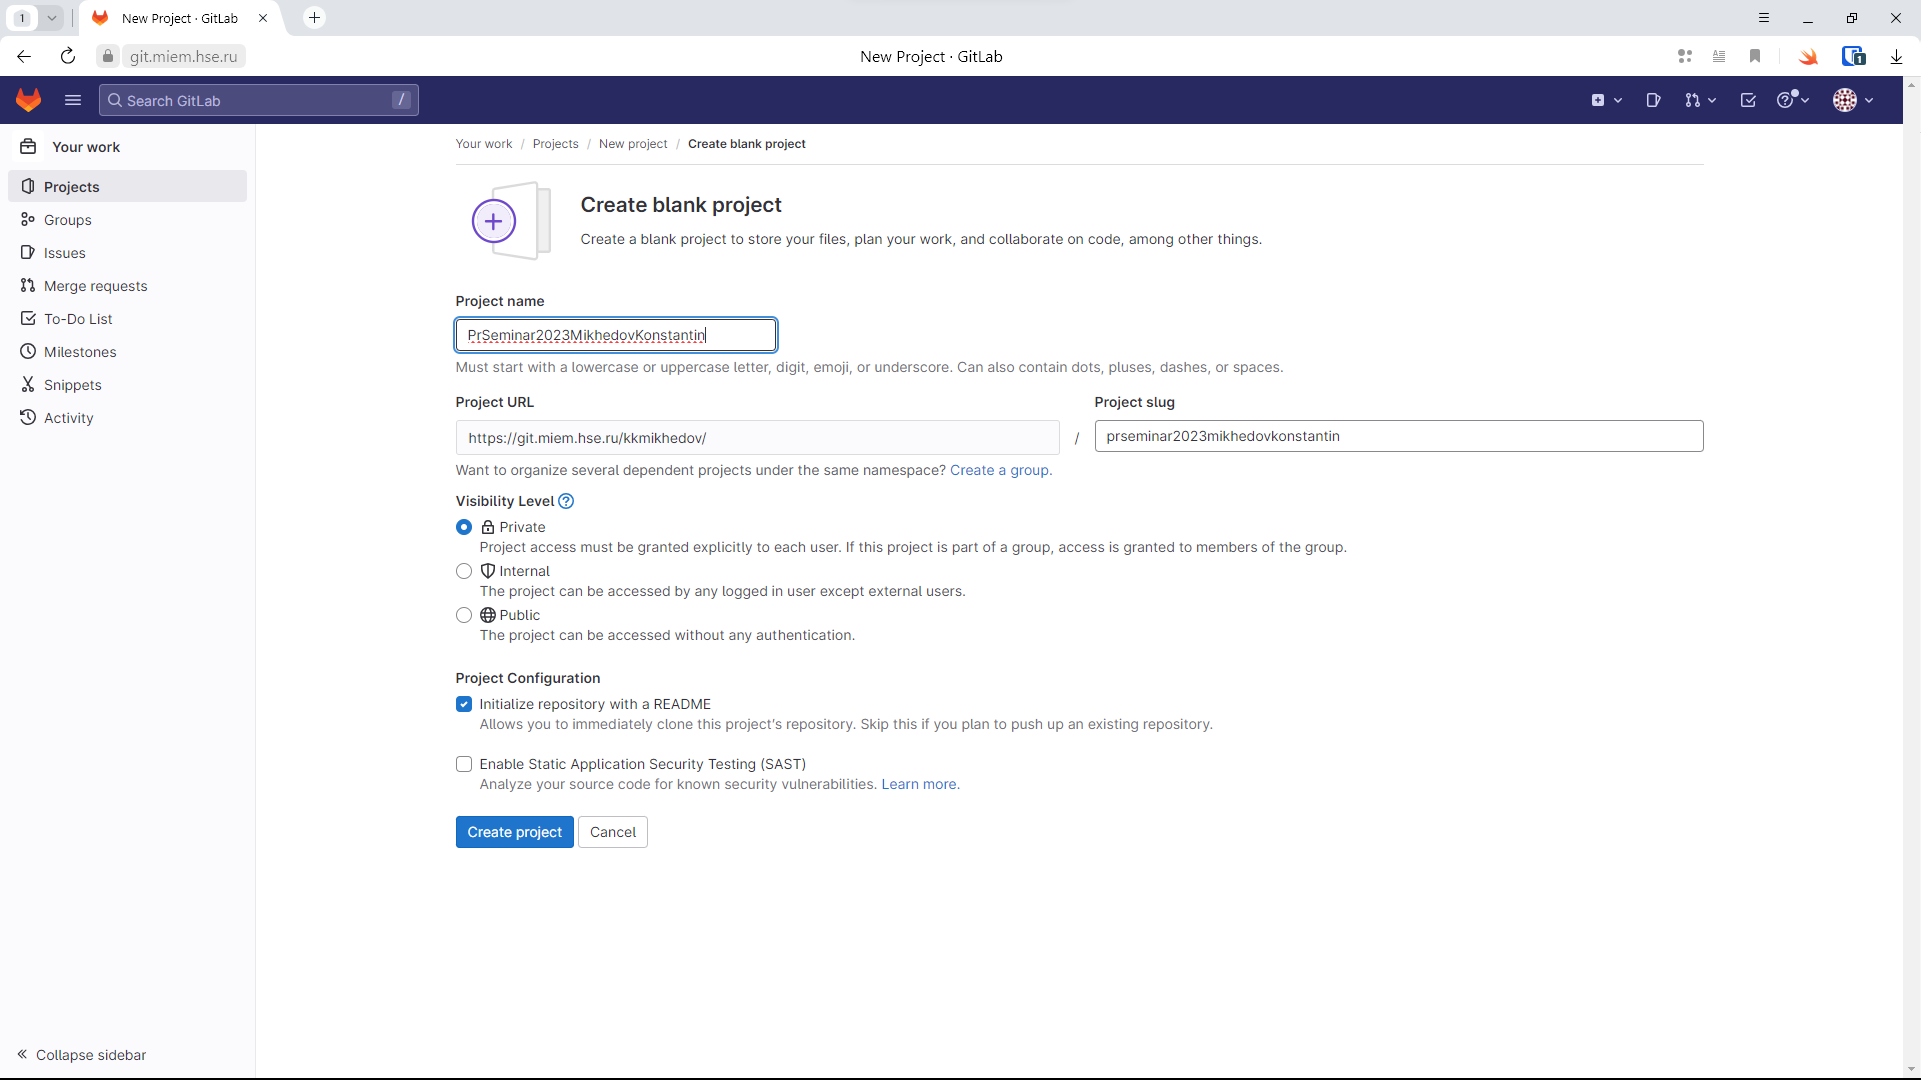
\includegraphics[width=\textwidth]{1_ (58)}
    \caption{Указываем имя и тип репозитория}
  \end{figure}

  \begin{figure}[H]
    \centering
    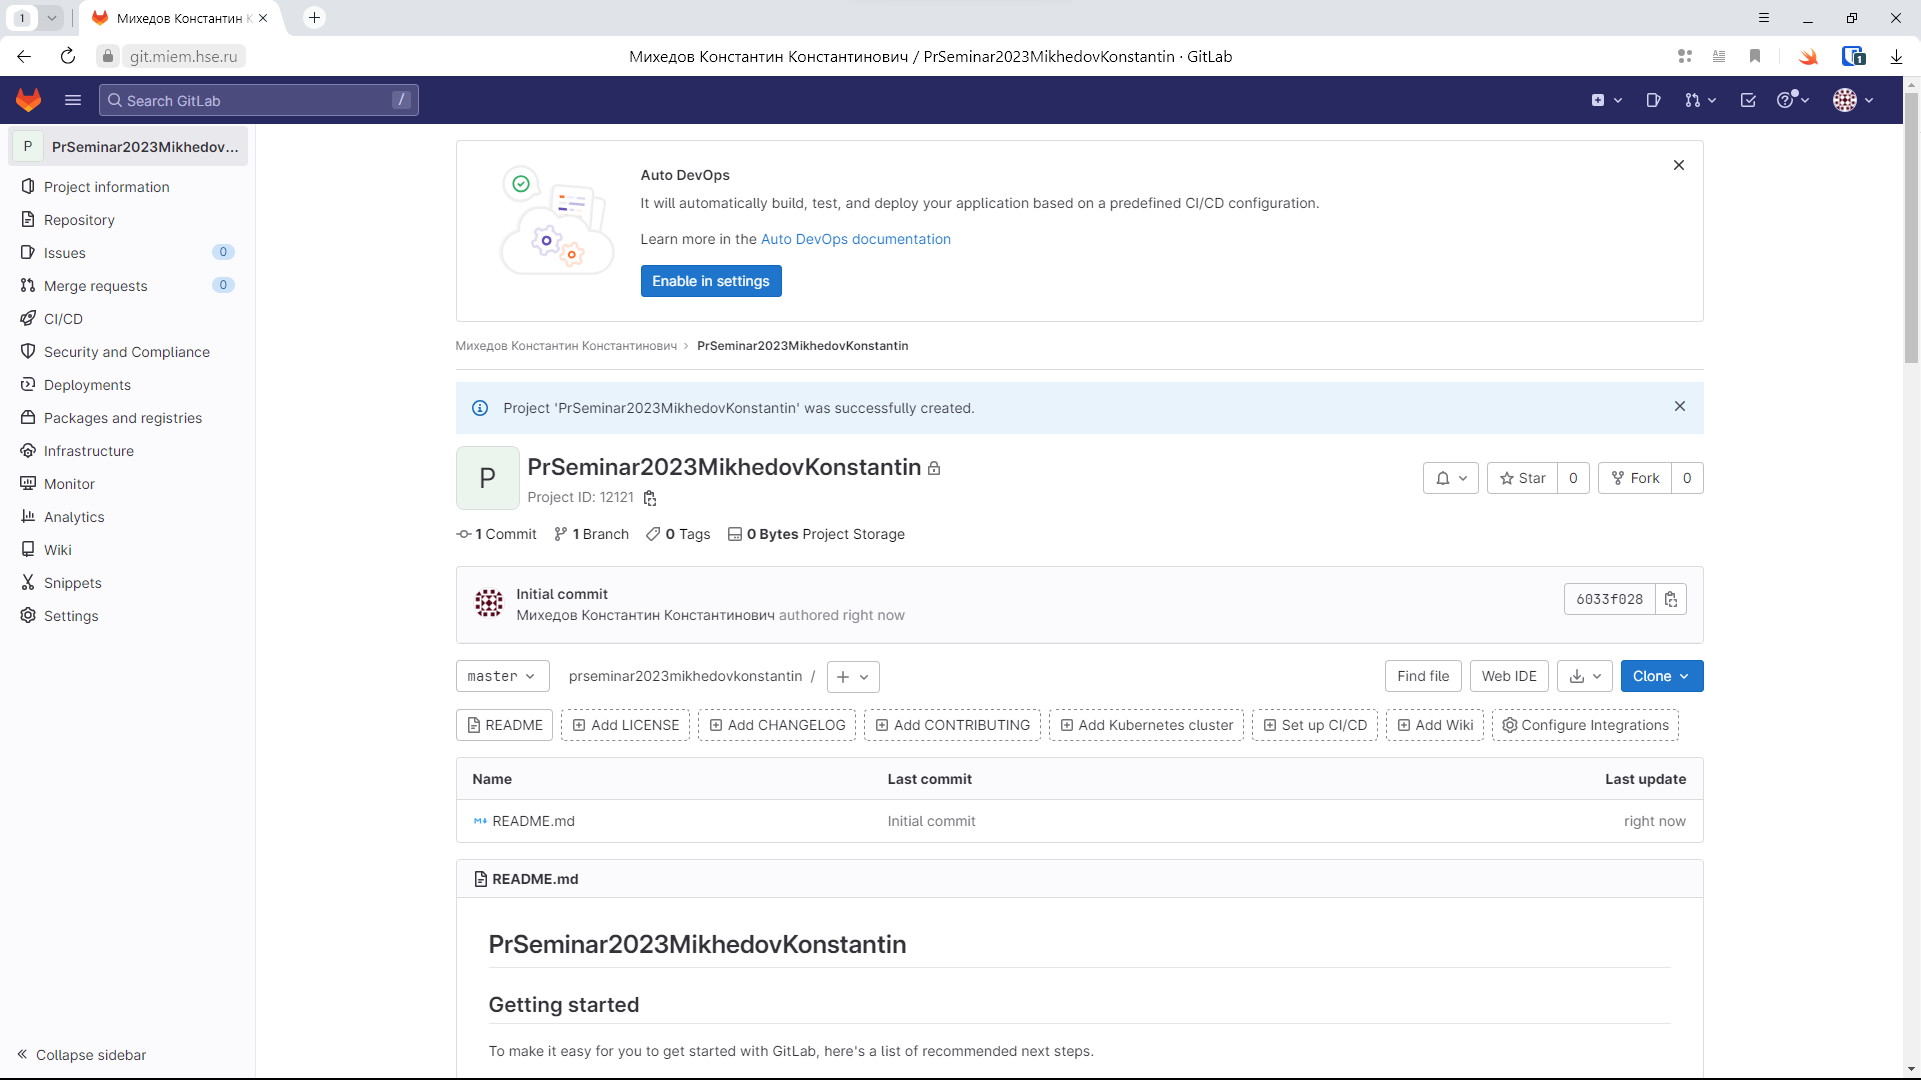
\includegraphics[width=\textwidth]{1_ (57)}
    \caption{Репозиторий создан и готов к работе}
  \end{figure}

  \subsection{Настройка доступов к репозиторию}

  \begin{figure}[H]
    \centering
    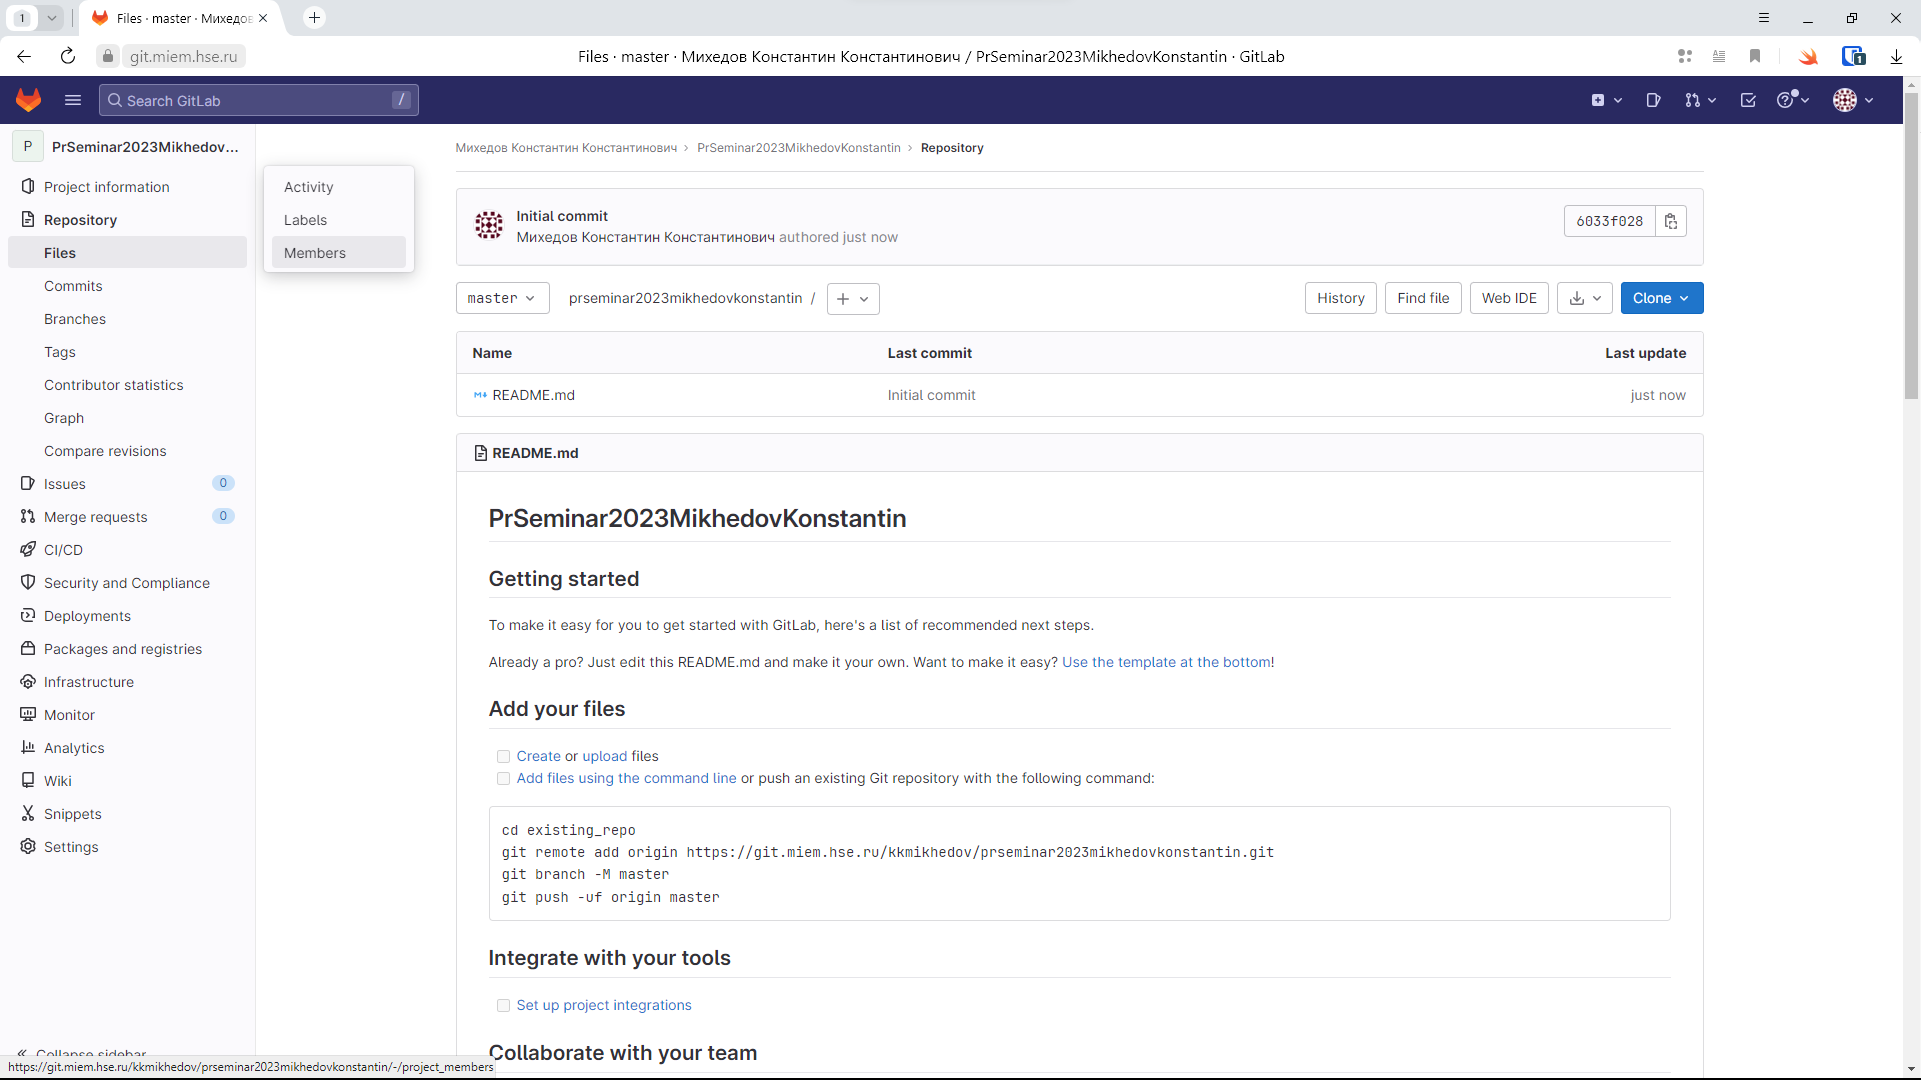
\includegraphics[width=\textwidth]{1_ (55)}
    \caption{Переходим к списку участников проекта}
  \end{figure}

  \begin{figure}[H]
    \centering
    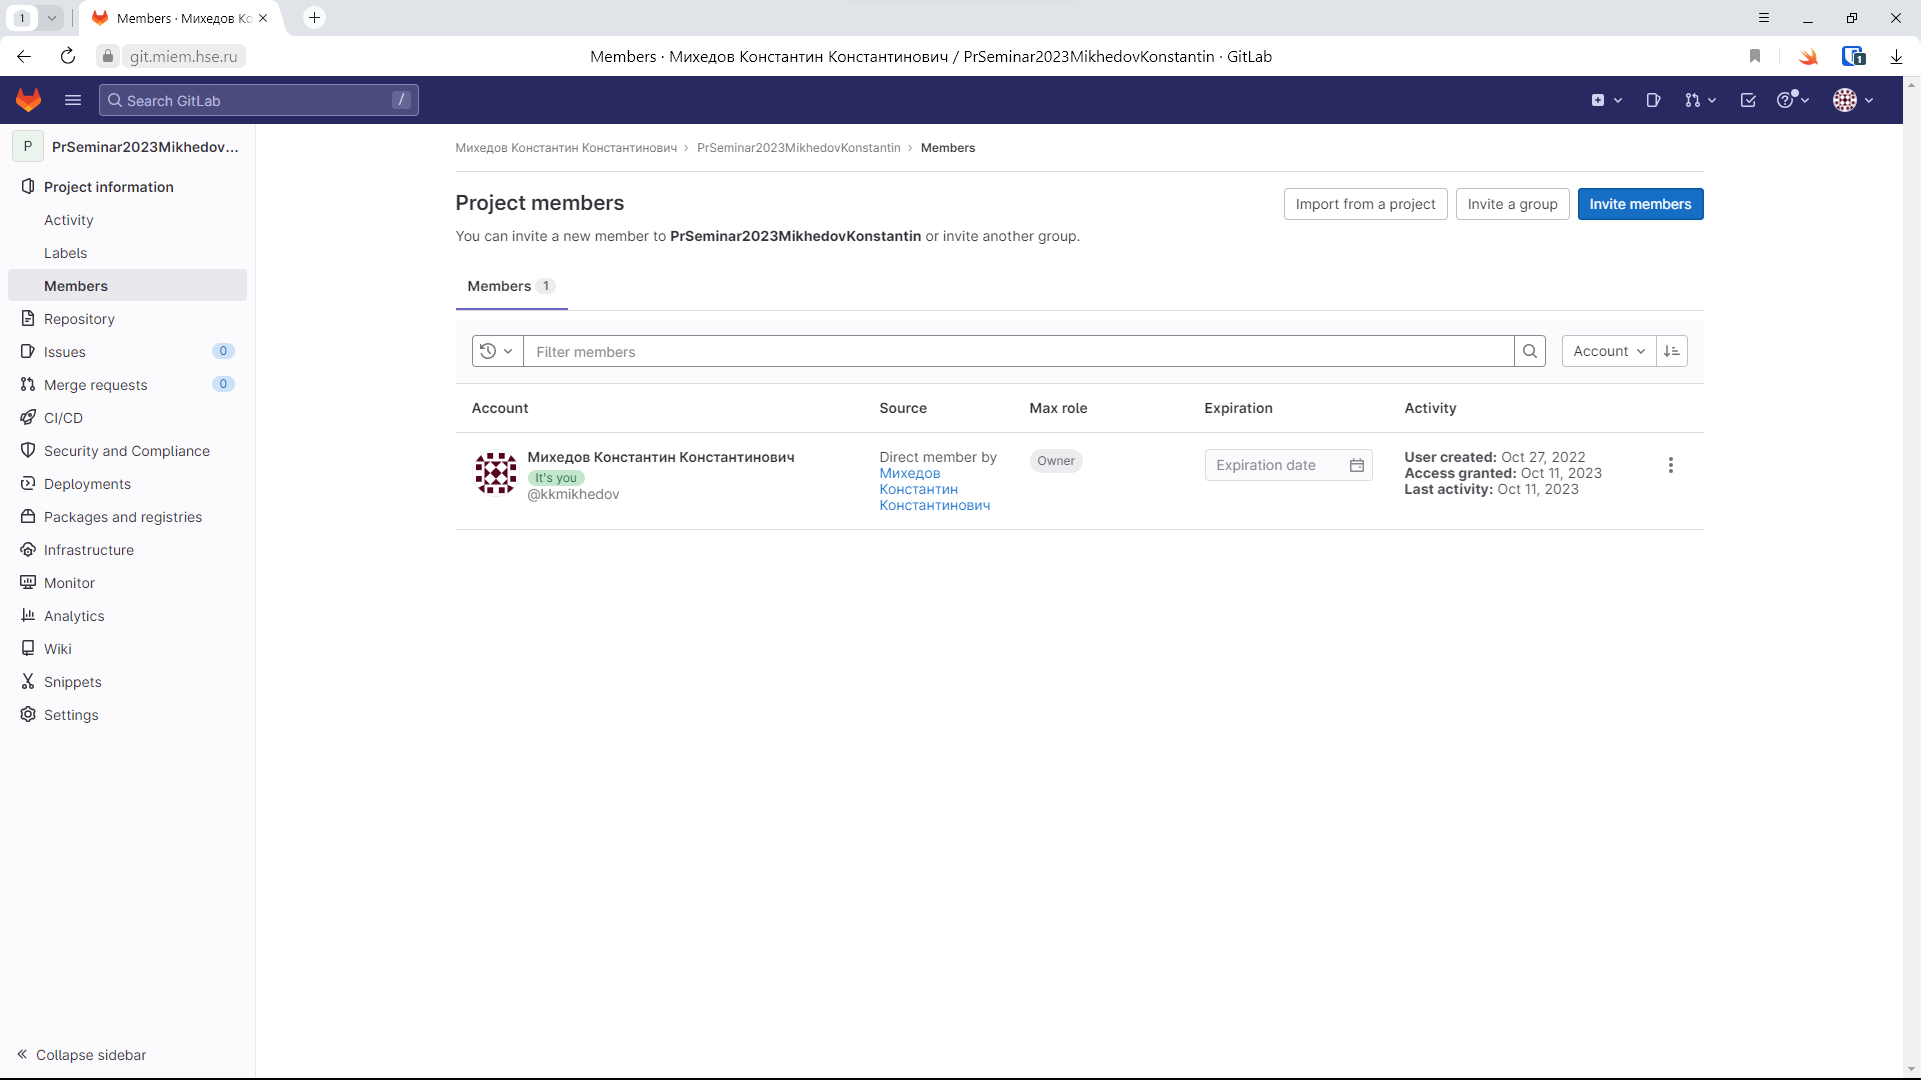
\includegraphics[width=\textwidth]{1_ (54)}
    \caption{Нажимаем кнопку <<Invite members>>}
  \end{figure}

  \begin{figure}[H]
    \centering
    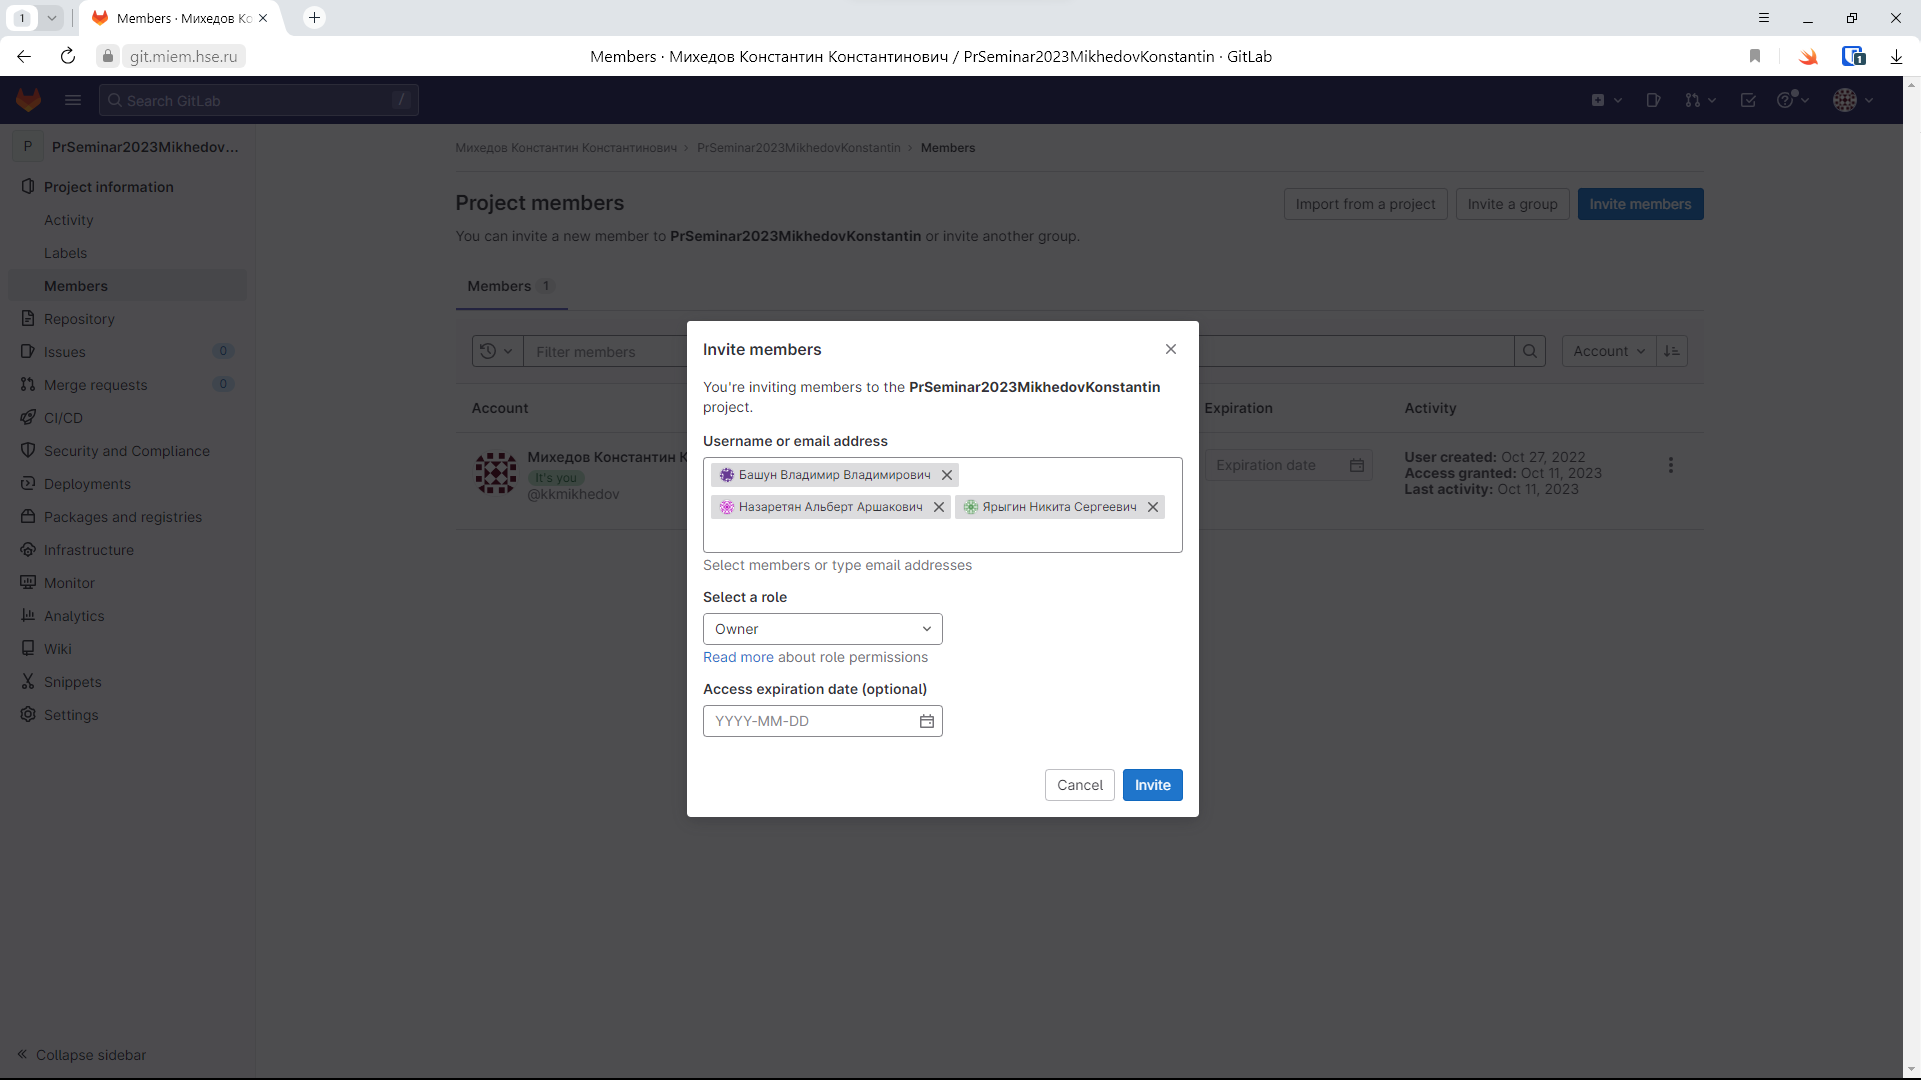
\includegraphics[width=\textwidth]{1_ (52)}
    \caption{Указываем необходимых пользователь и роль <<Owner>> для них}
  \end{figure}

  \begin{figure}[H]
    \centering
    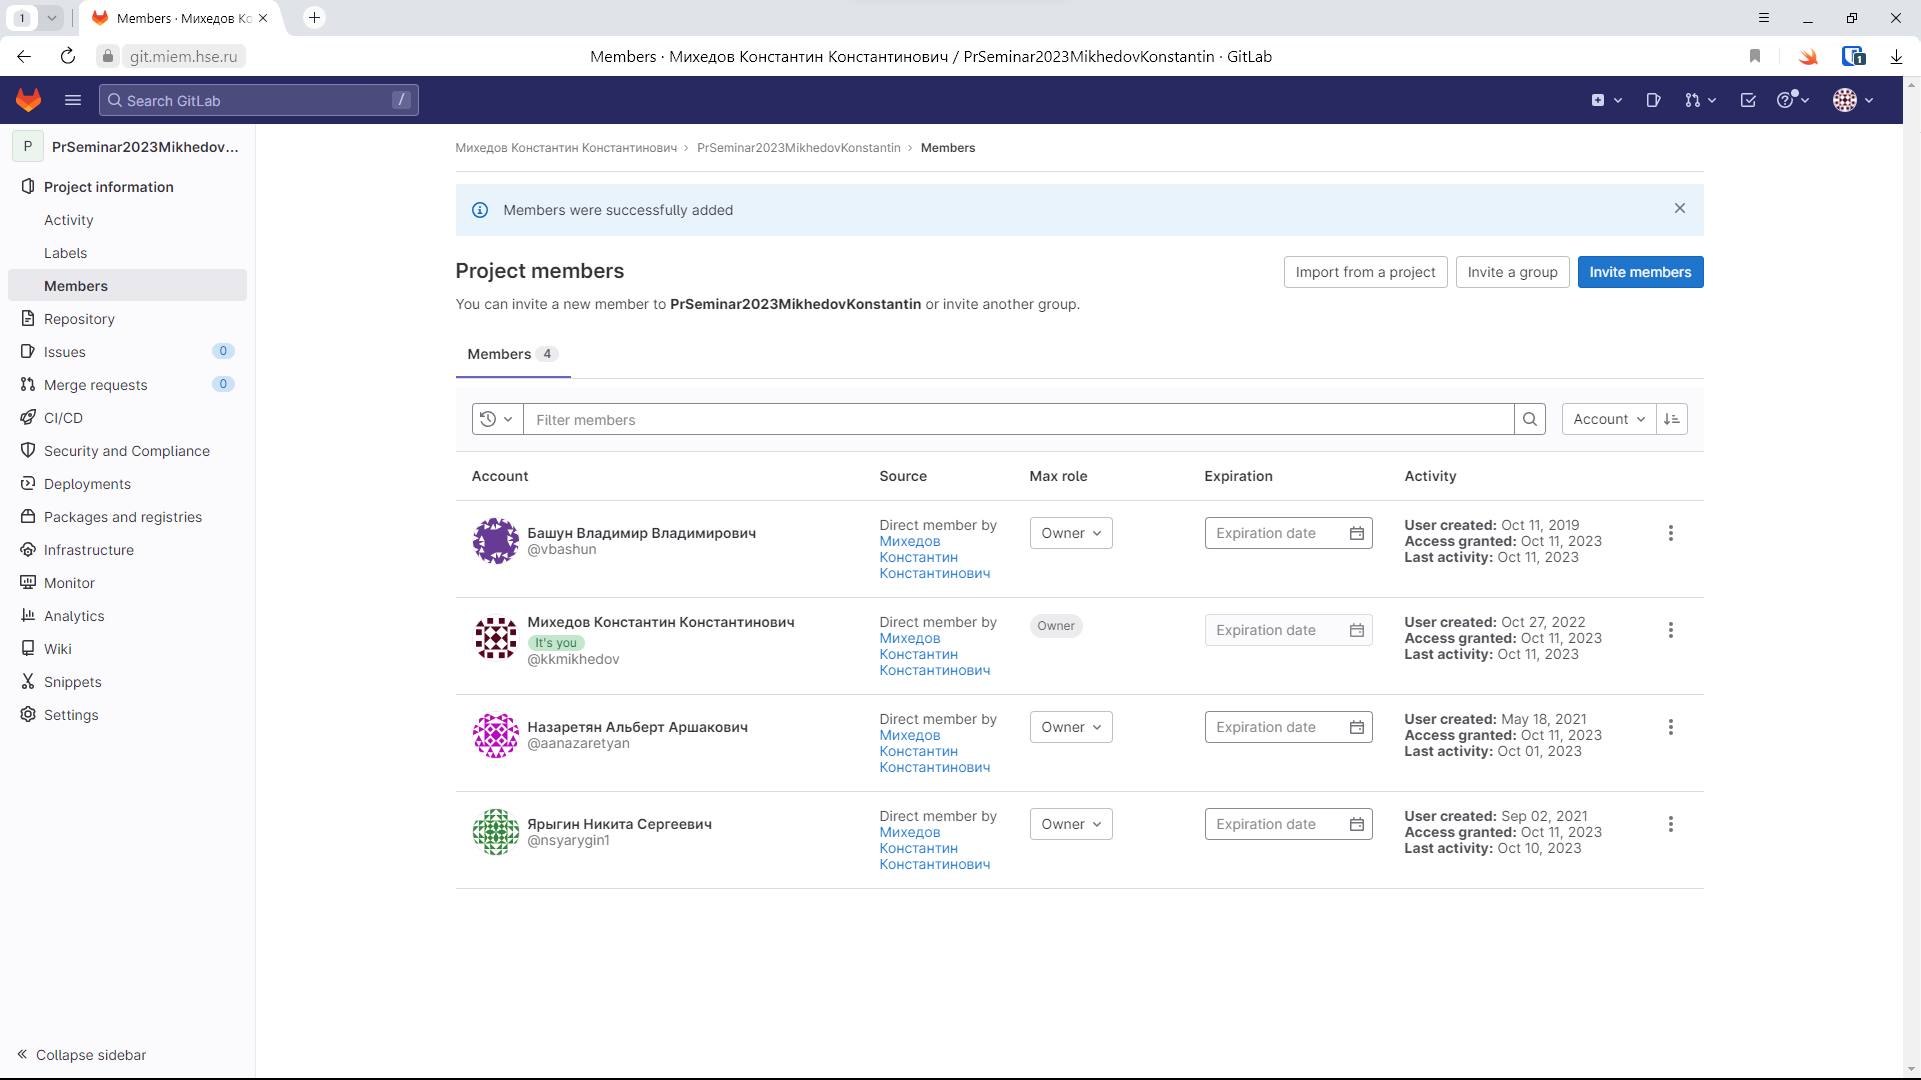
\includegraphics[width=\textwidth]{1_ (51)}
    \caption{Пользователи появились}
  \end{figure}

  \begin{figure}[H]
    \centering
    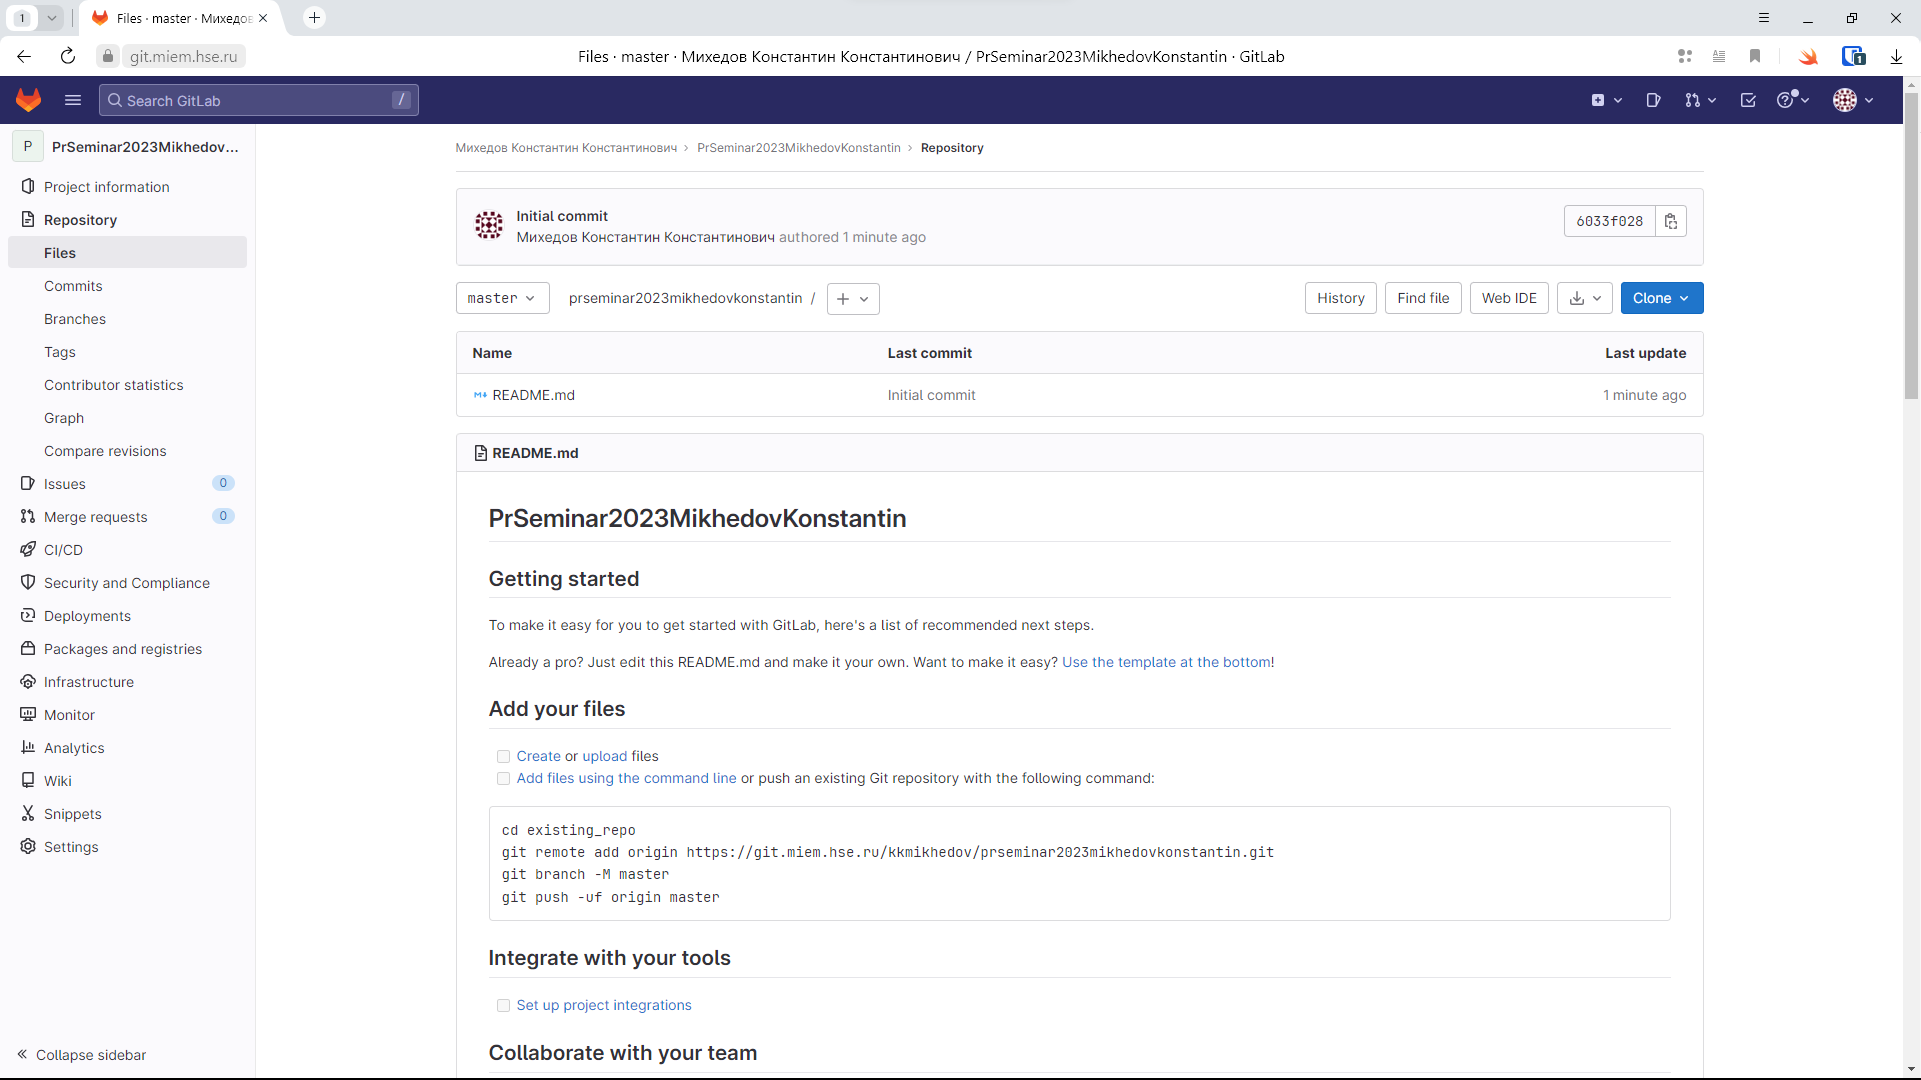
\includegraphics[width=\textwidth]{1_ (50)}
    \caption{Готовый к работе репозиторий}
  \end{figure}

  \subsection{Создание ветки develop}

  \begin{figure}[H]
    \centering
    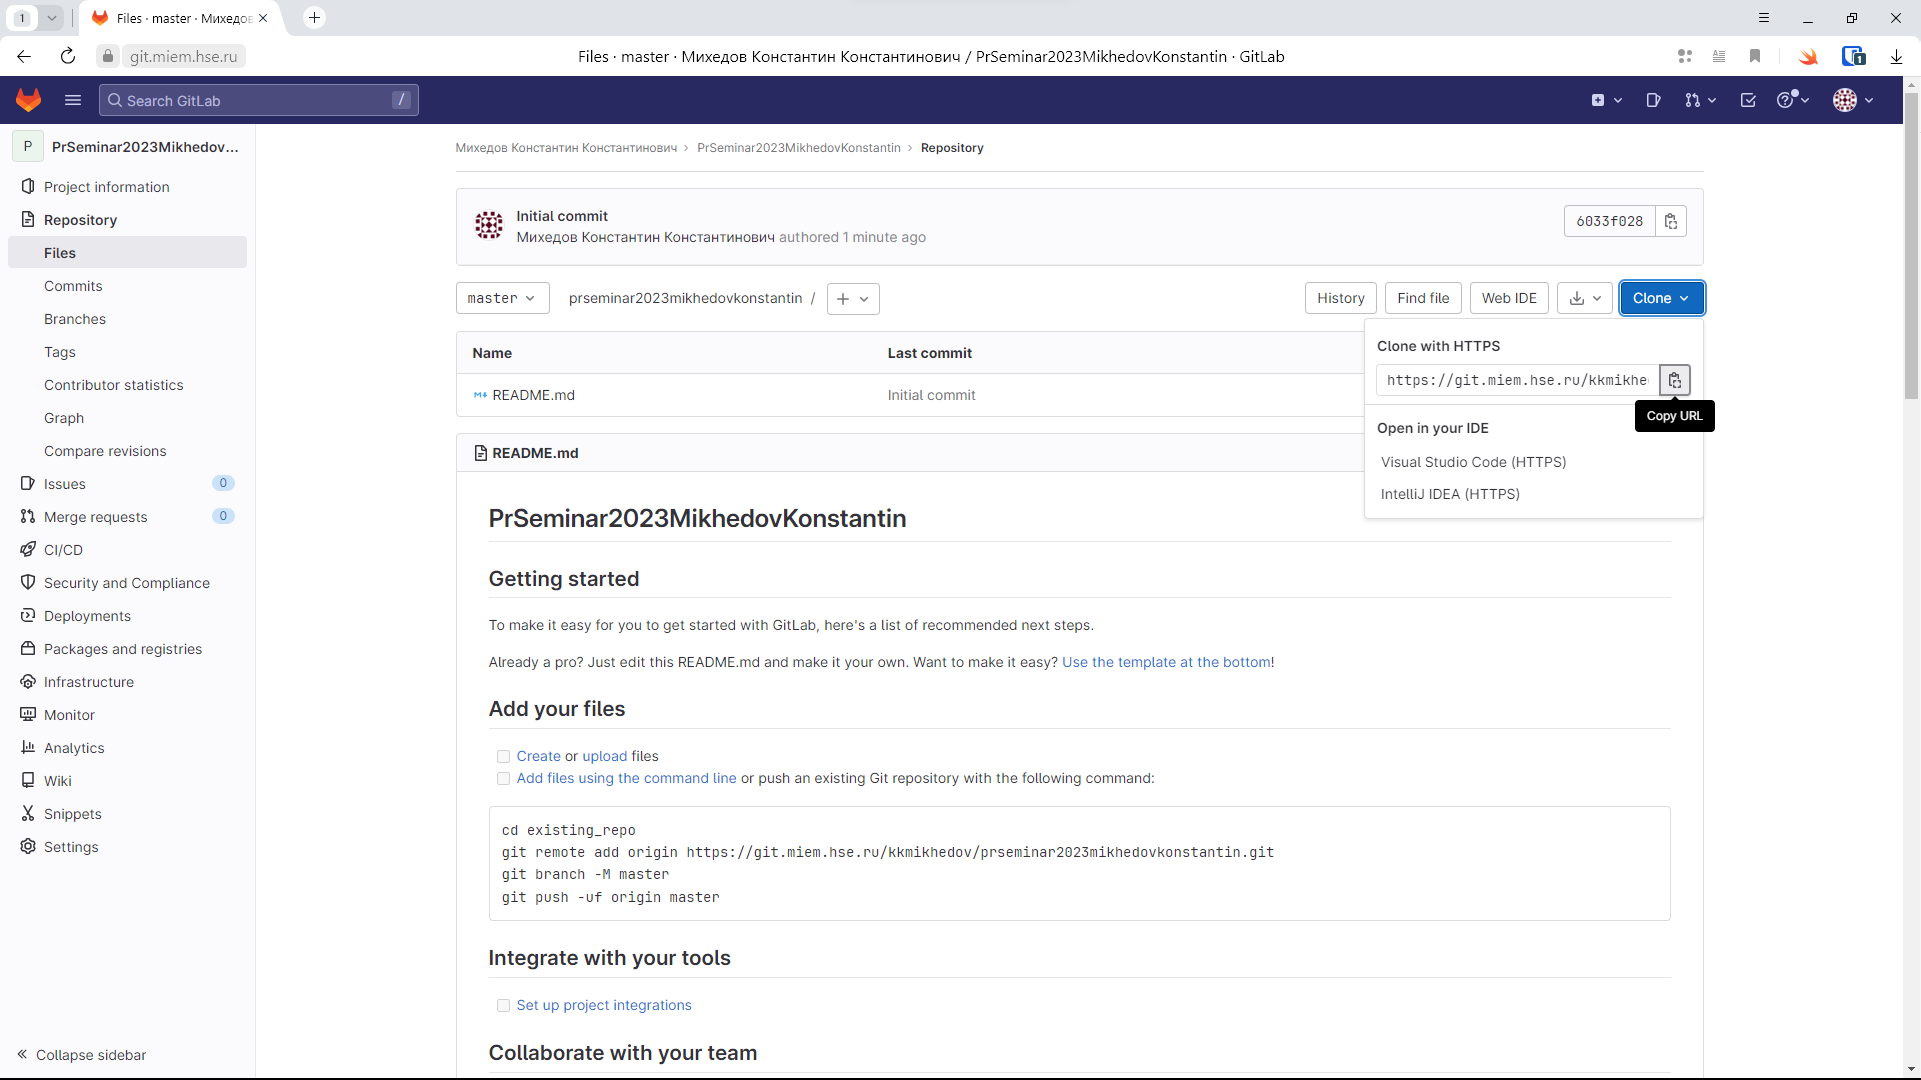
\includegraphics[width=\textwidth]{1_ (49)}
    \caption{Копируем ссылку для клонирования репозитория}
  \end{figure}

  \begin{figure}[H]
    \centering
    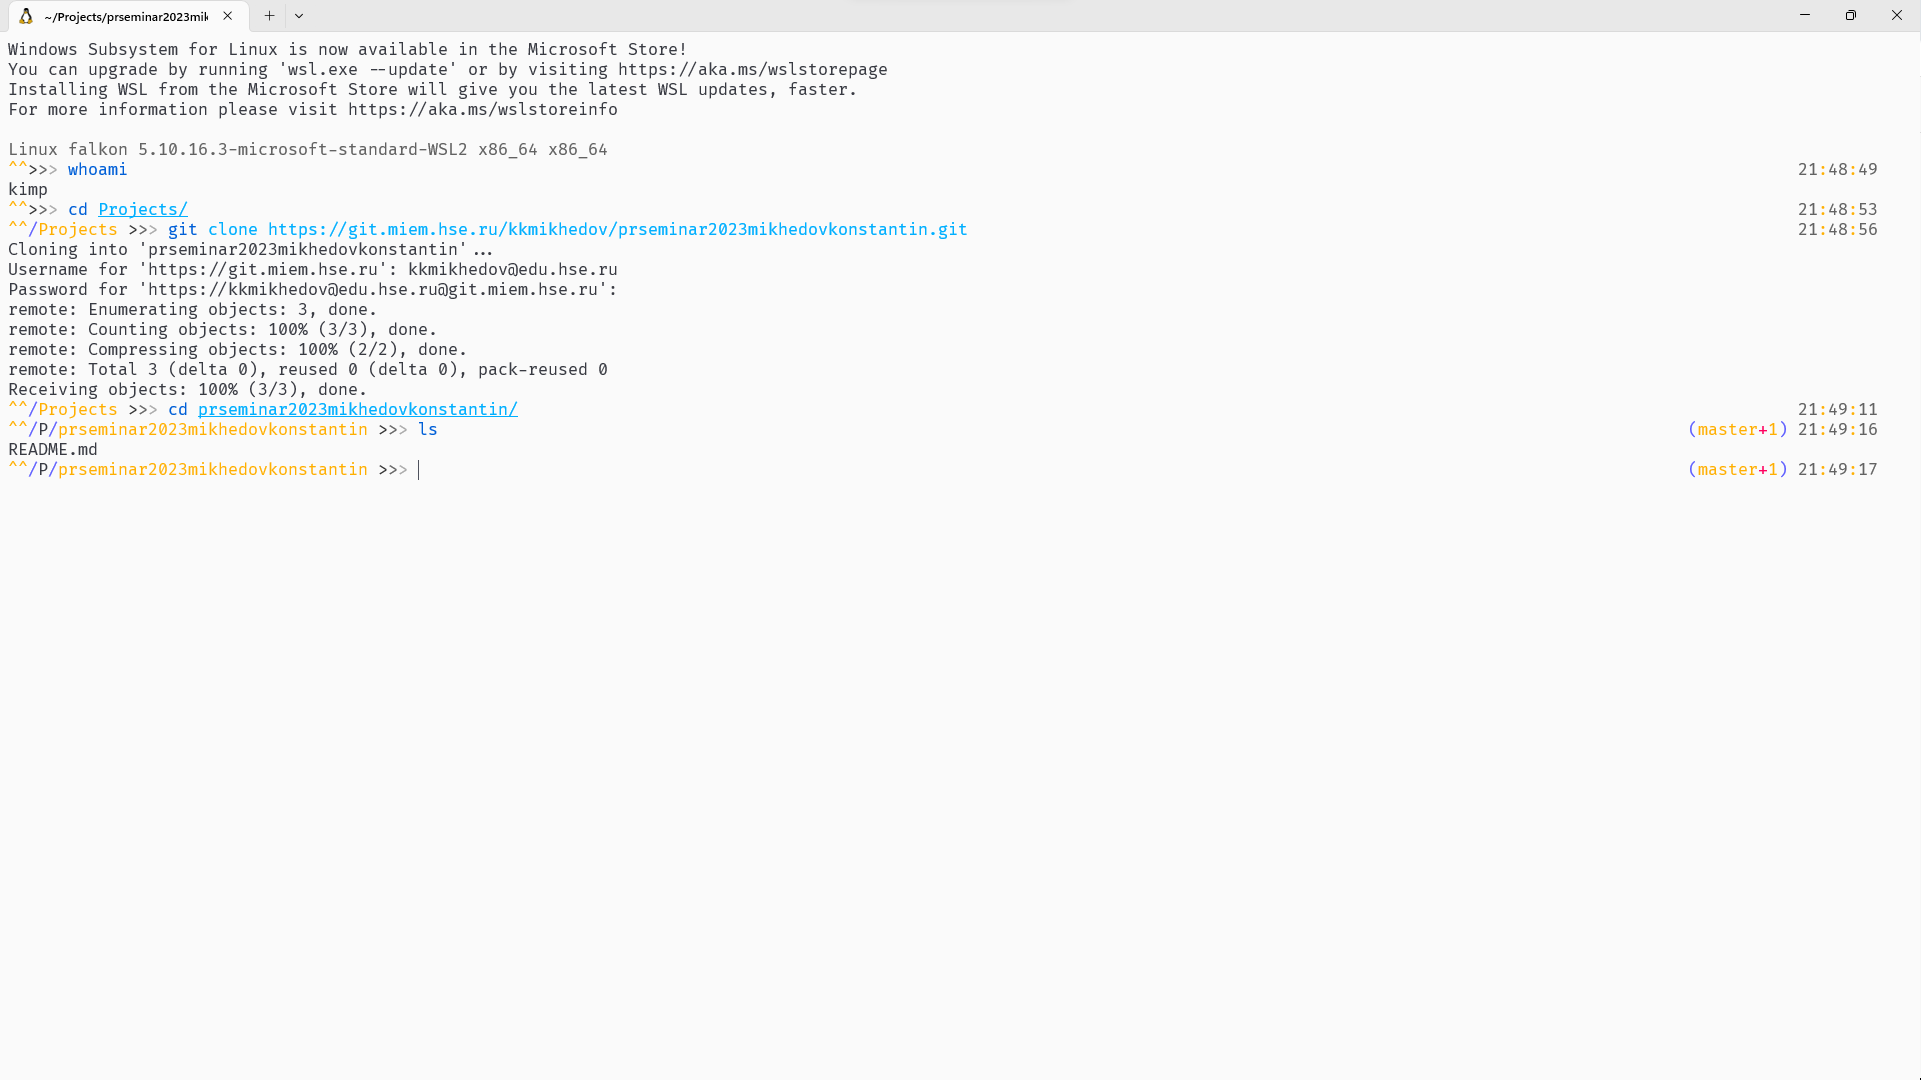
\includegraphics[width=\textwidth]{1_ (48)}
    \caption{Клонируем репозиторий при помощи git clone}
  \end{figure}

  \begin{figure}[H]
    \centering
    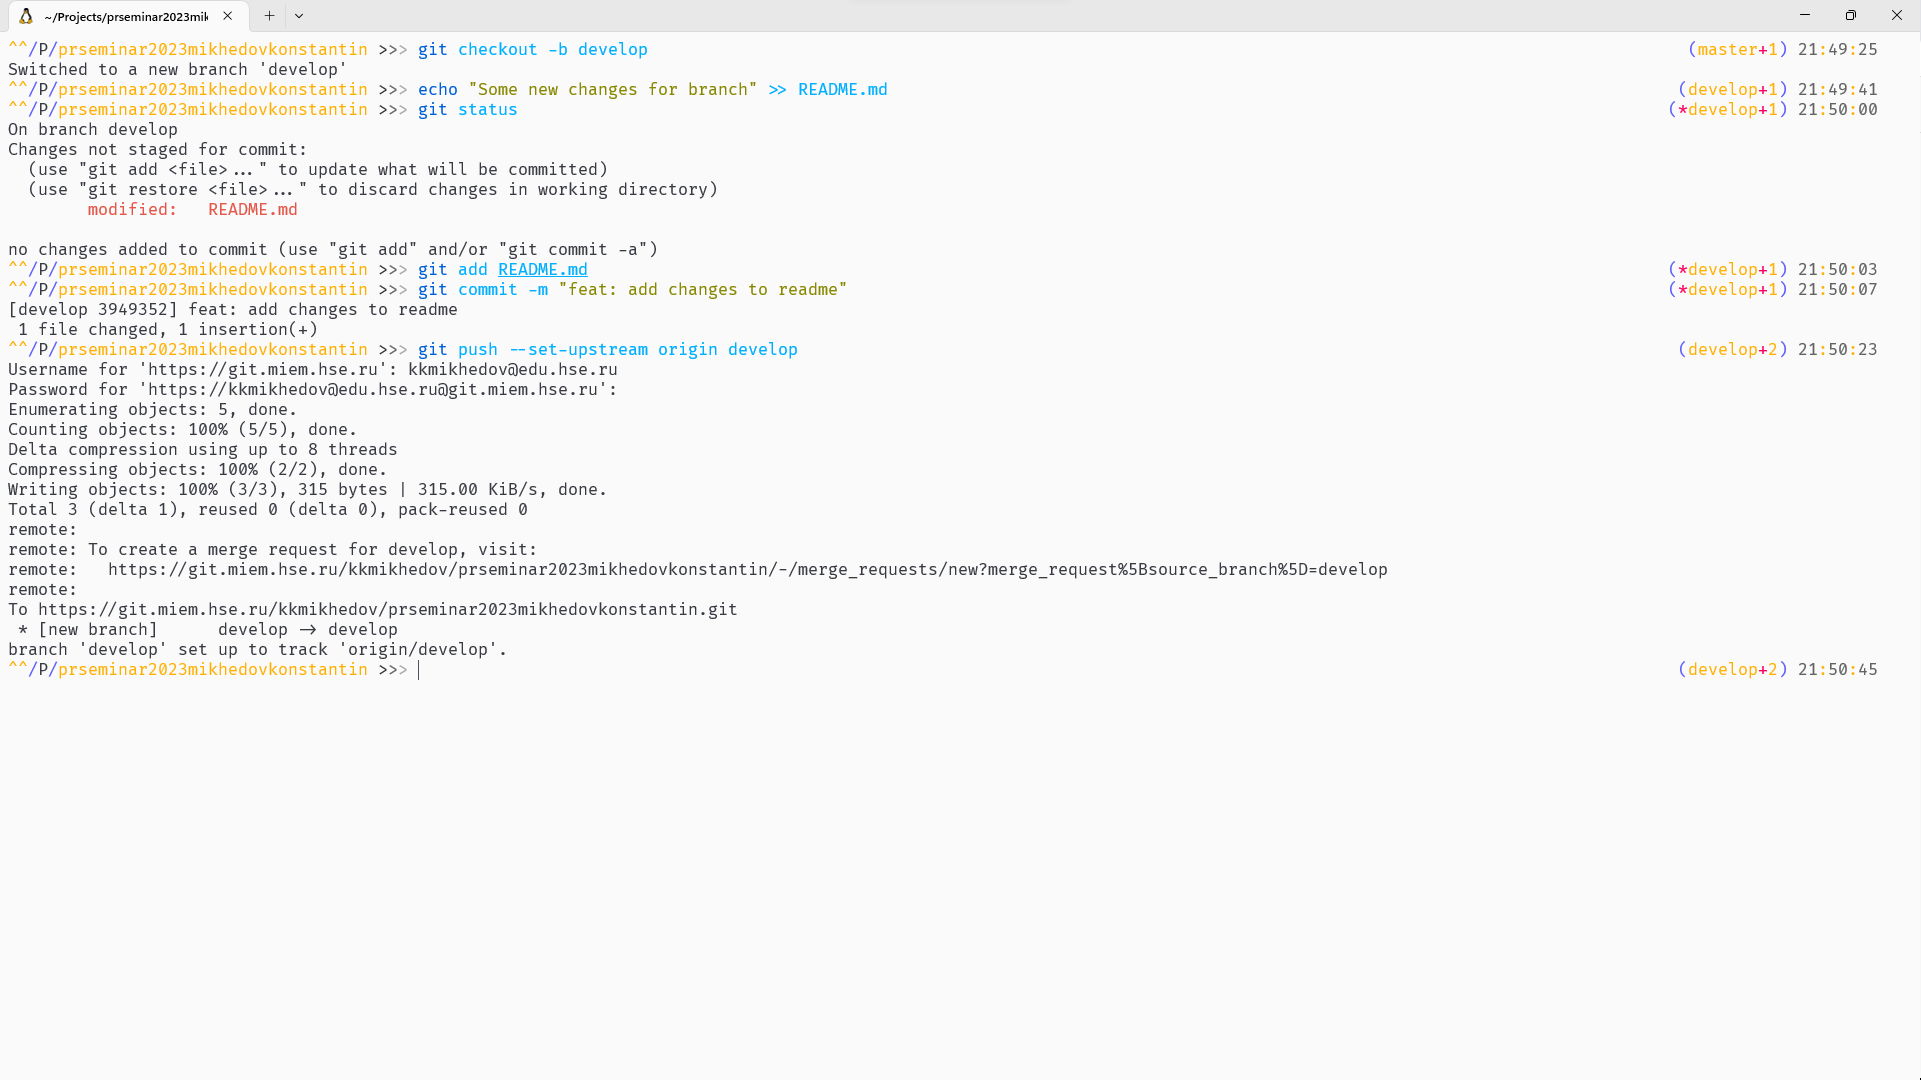
\includegraphics[width=\textwidth]{1_ (47)}
    \caption{Вносим изменения в README.md, коммитим изменения и пушим в удаленный репозиторий}
  \end{figure}

  \begin{figure}[H]
    \centering
    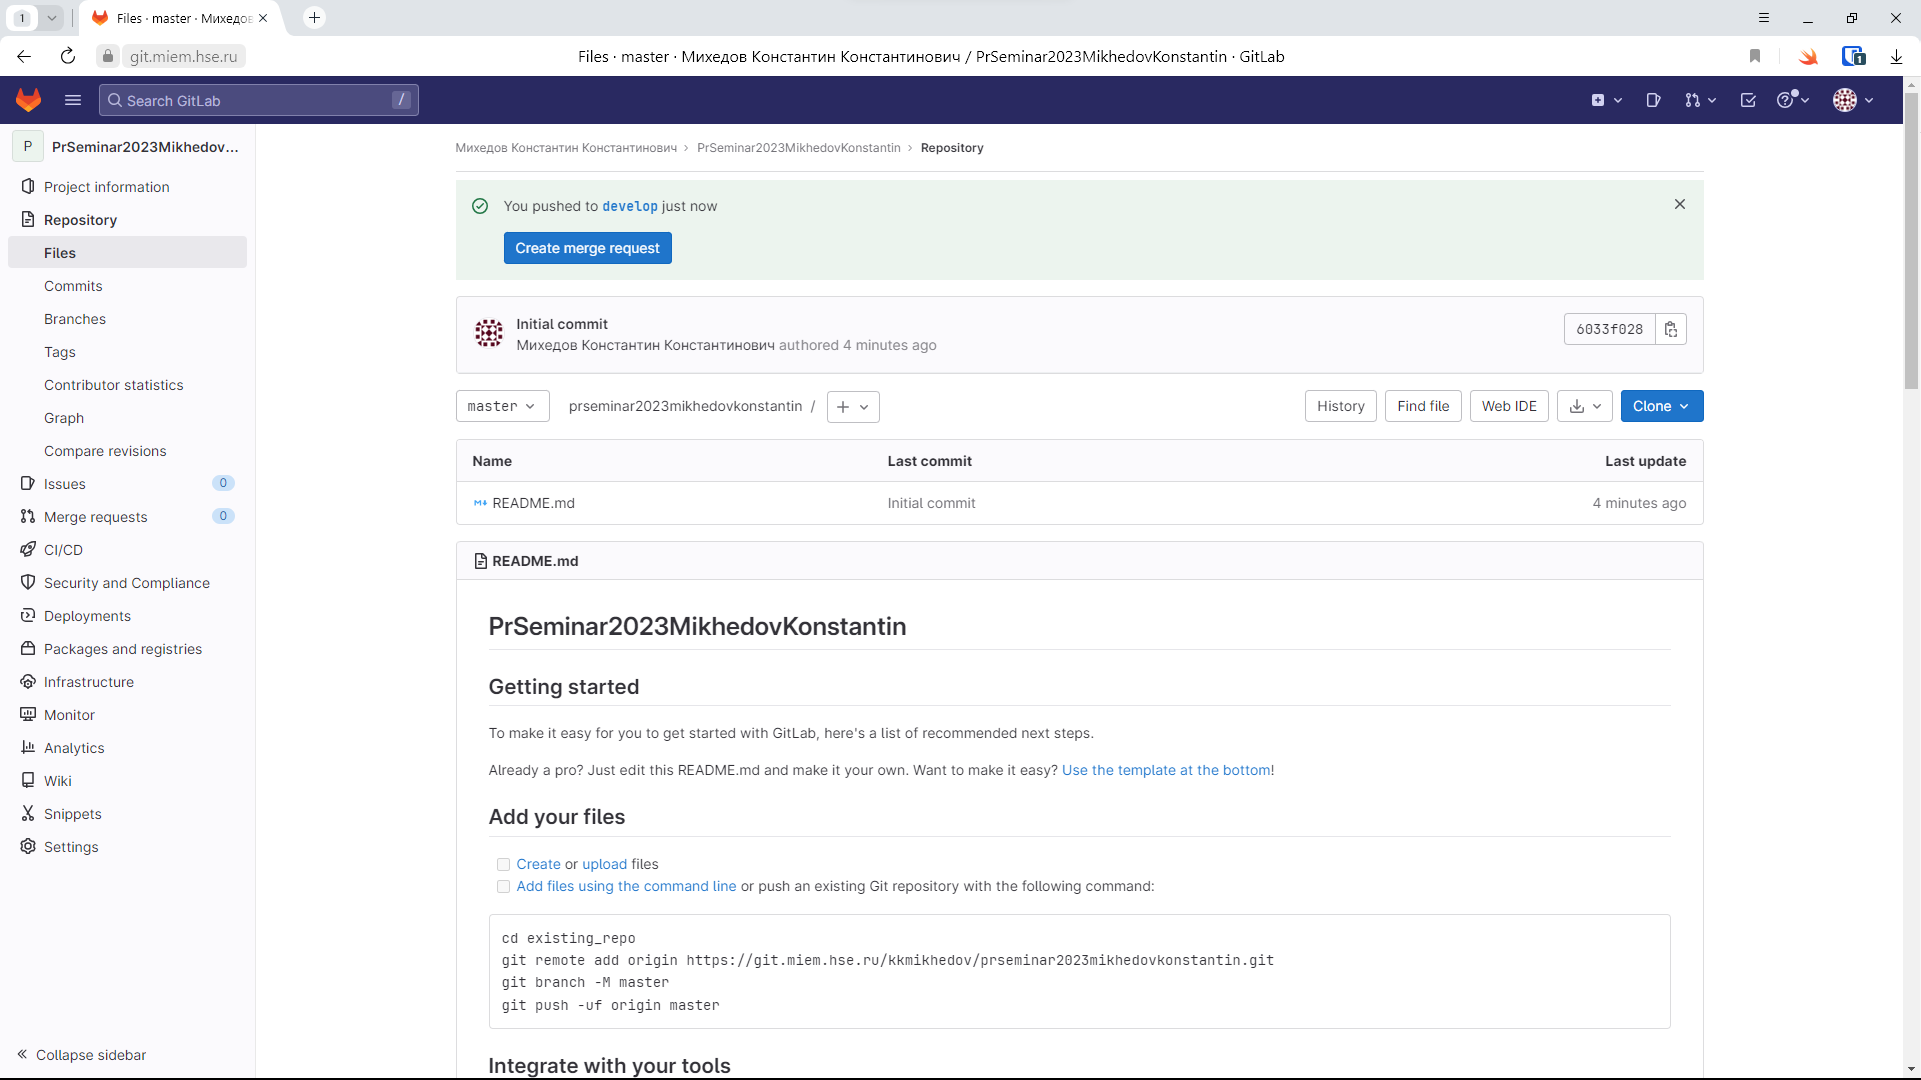
\includegraphics[width=\textwidth]{1_ (46)}
    \caption{Новая ветка проросла в интерфейсе}
  \end{figure}

  \begin{figure}[H]
    \centering
    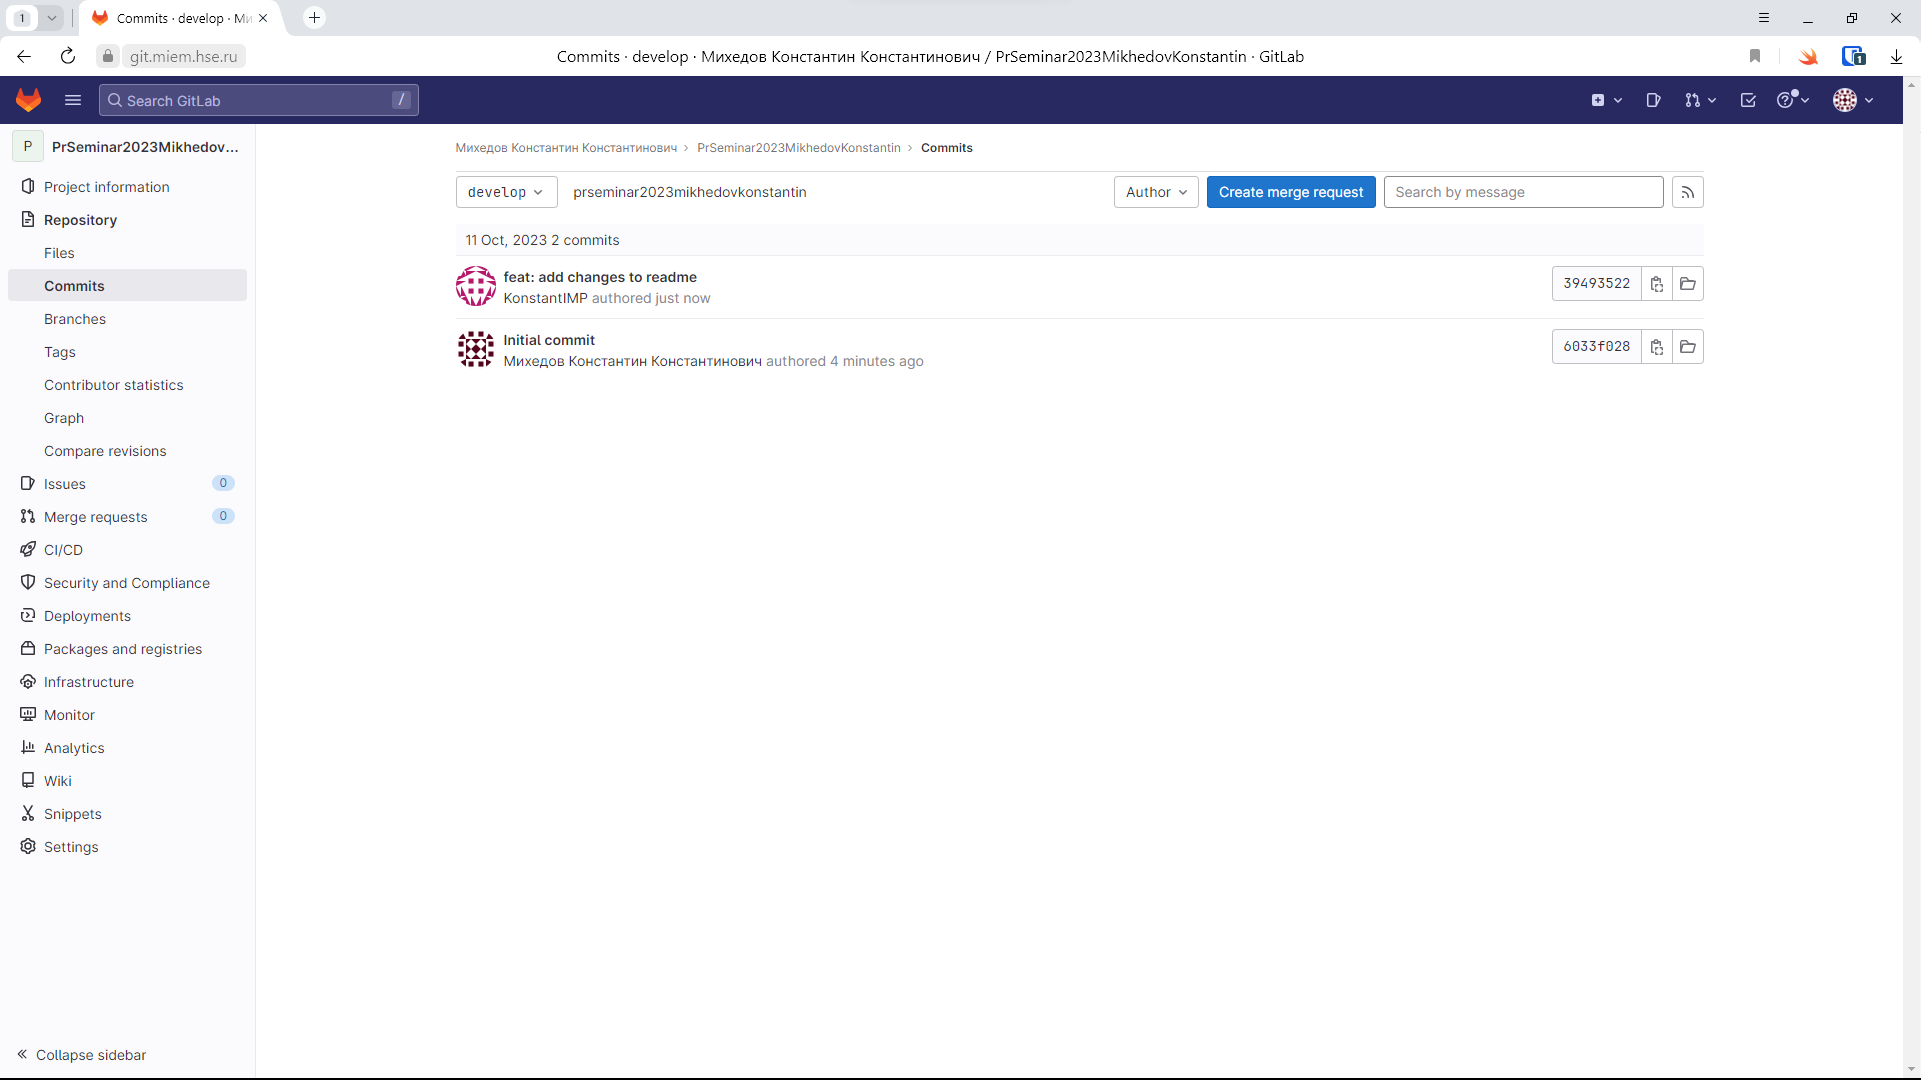
\includegraphics[width=\textwidth]{1_ (45)}
    \caption{В изменениях ветки develop видно коммит}
  \end{figure}

  \subsection{Настройка push и merge доступов, ветки по умолчанию}

  \subsubsection{Настройка доступов. Попытка первая}

  \begin{figure}[H]
    \centering
    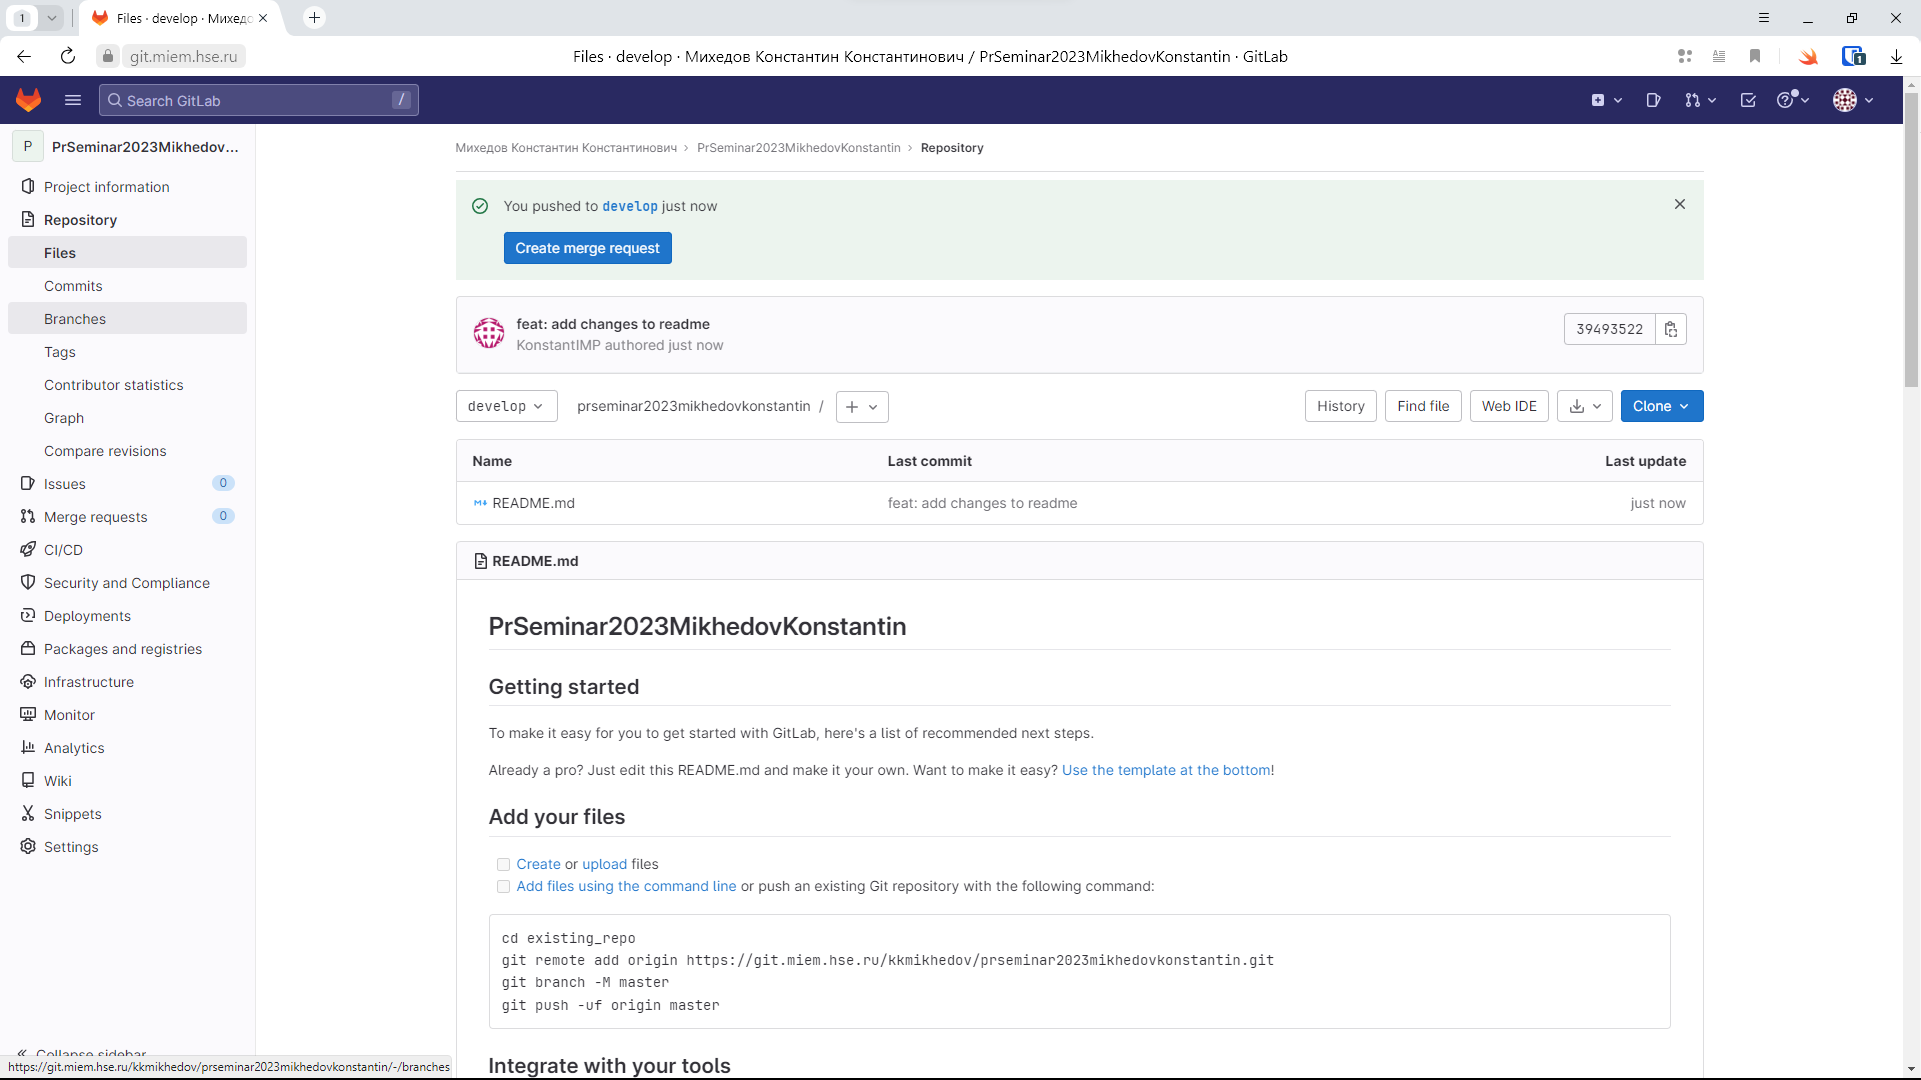
\includegraphics[width=\textwidth]{1_ (44)}
    \caption{Переходим на вкладку <<Branches>>}
  \end{figure}

  \begin{figure}[H]
    \centering
    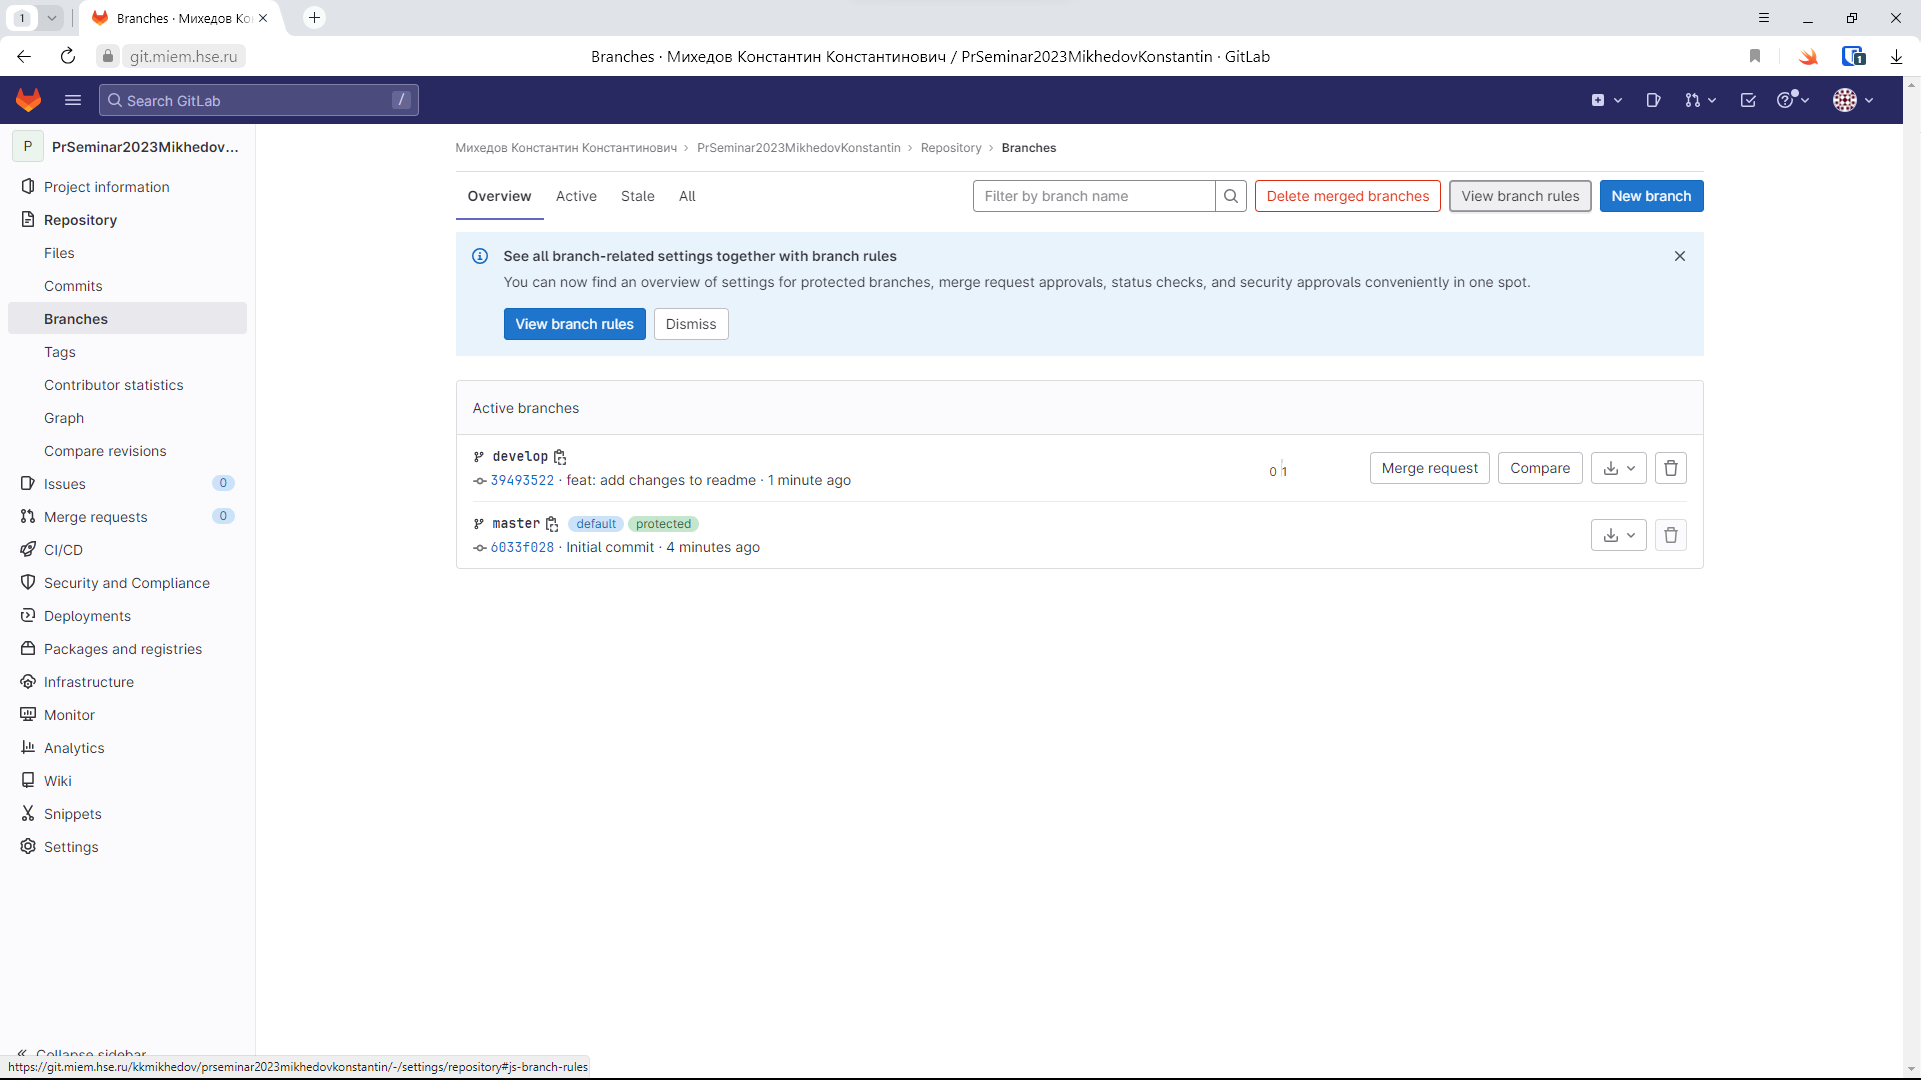
\includegraphics[width=\textwidth]{1_ (43)}
    \caption{Нажимаем кнопку <<View branch rules>>}
  \end{figure}

  \begin{figure}[H]
    \centering
    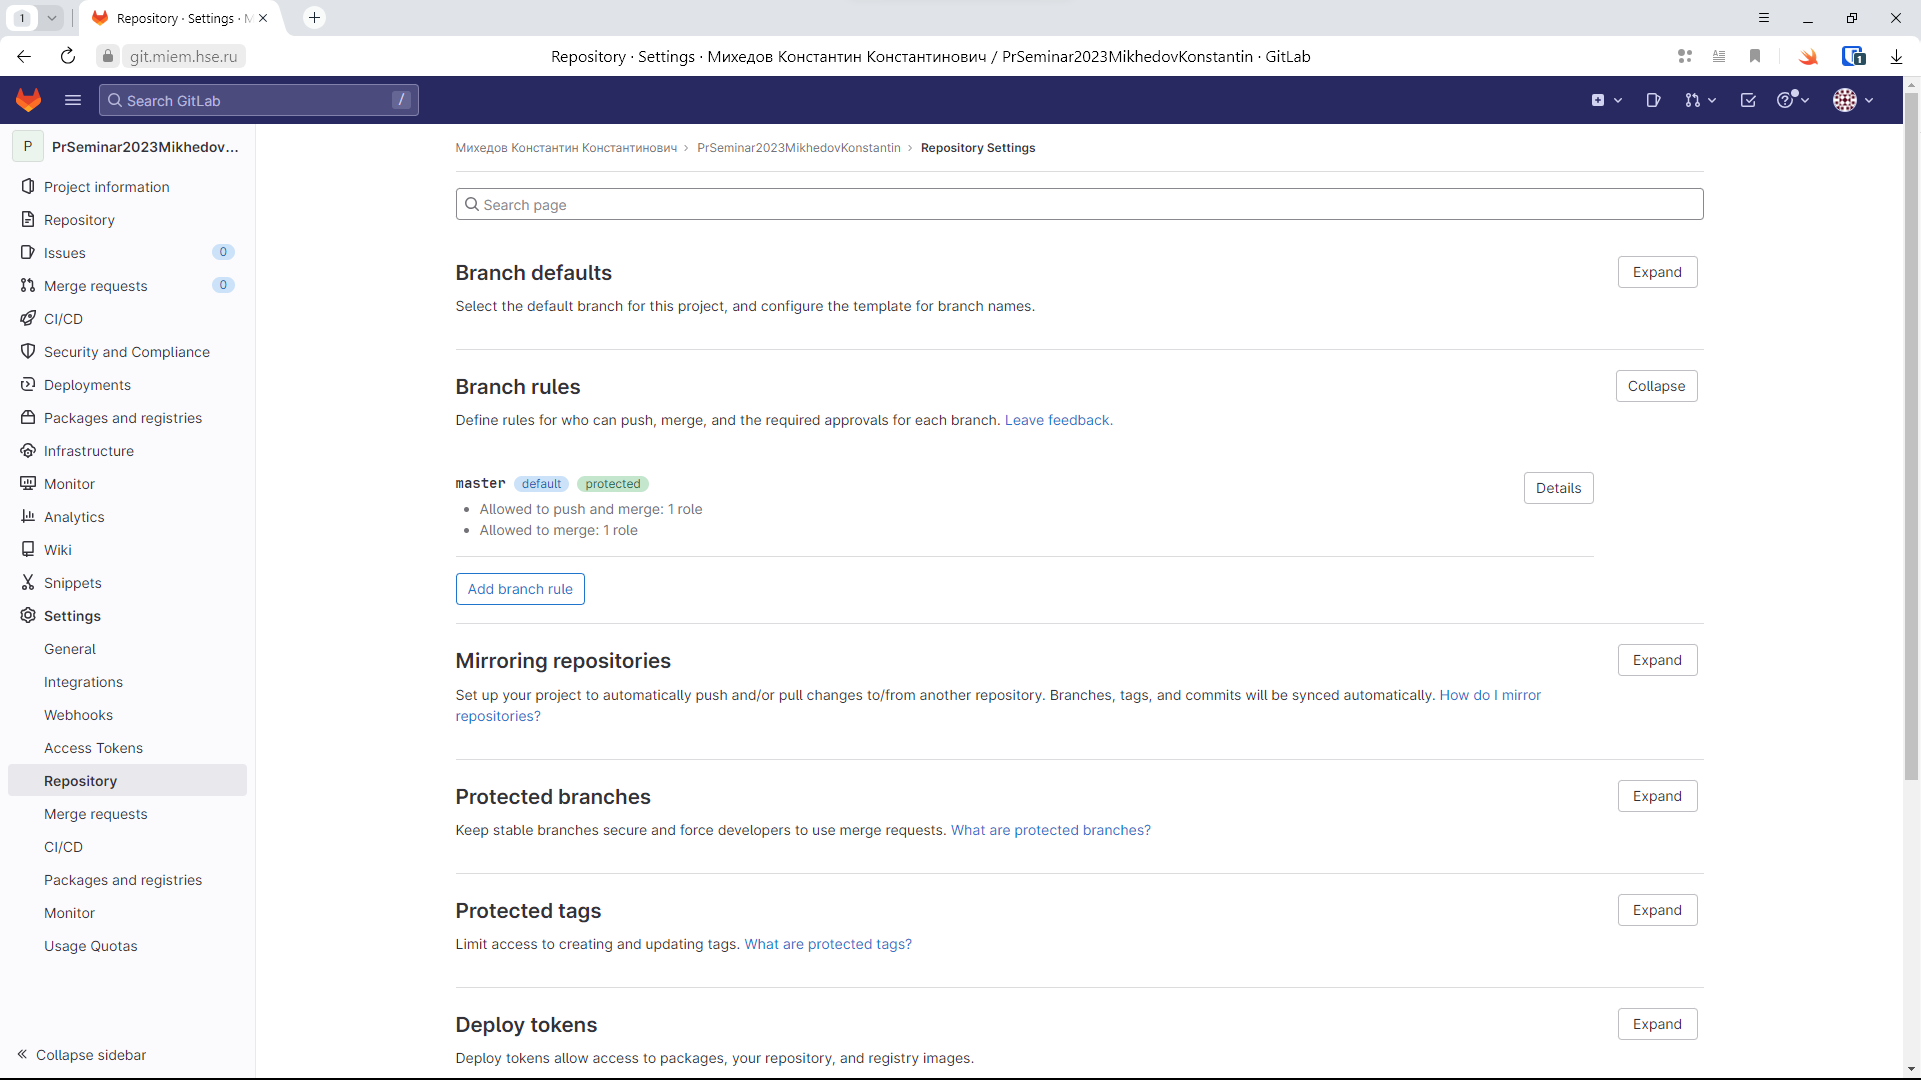
\includegraphics[width=\textwidth]{1_ (42)}
    \caption{Видим, что правила настроены только для ветки master}
  \end{figure}

  \begin{figure}[H]
    \centering
    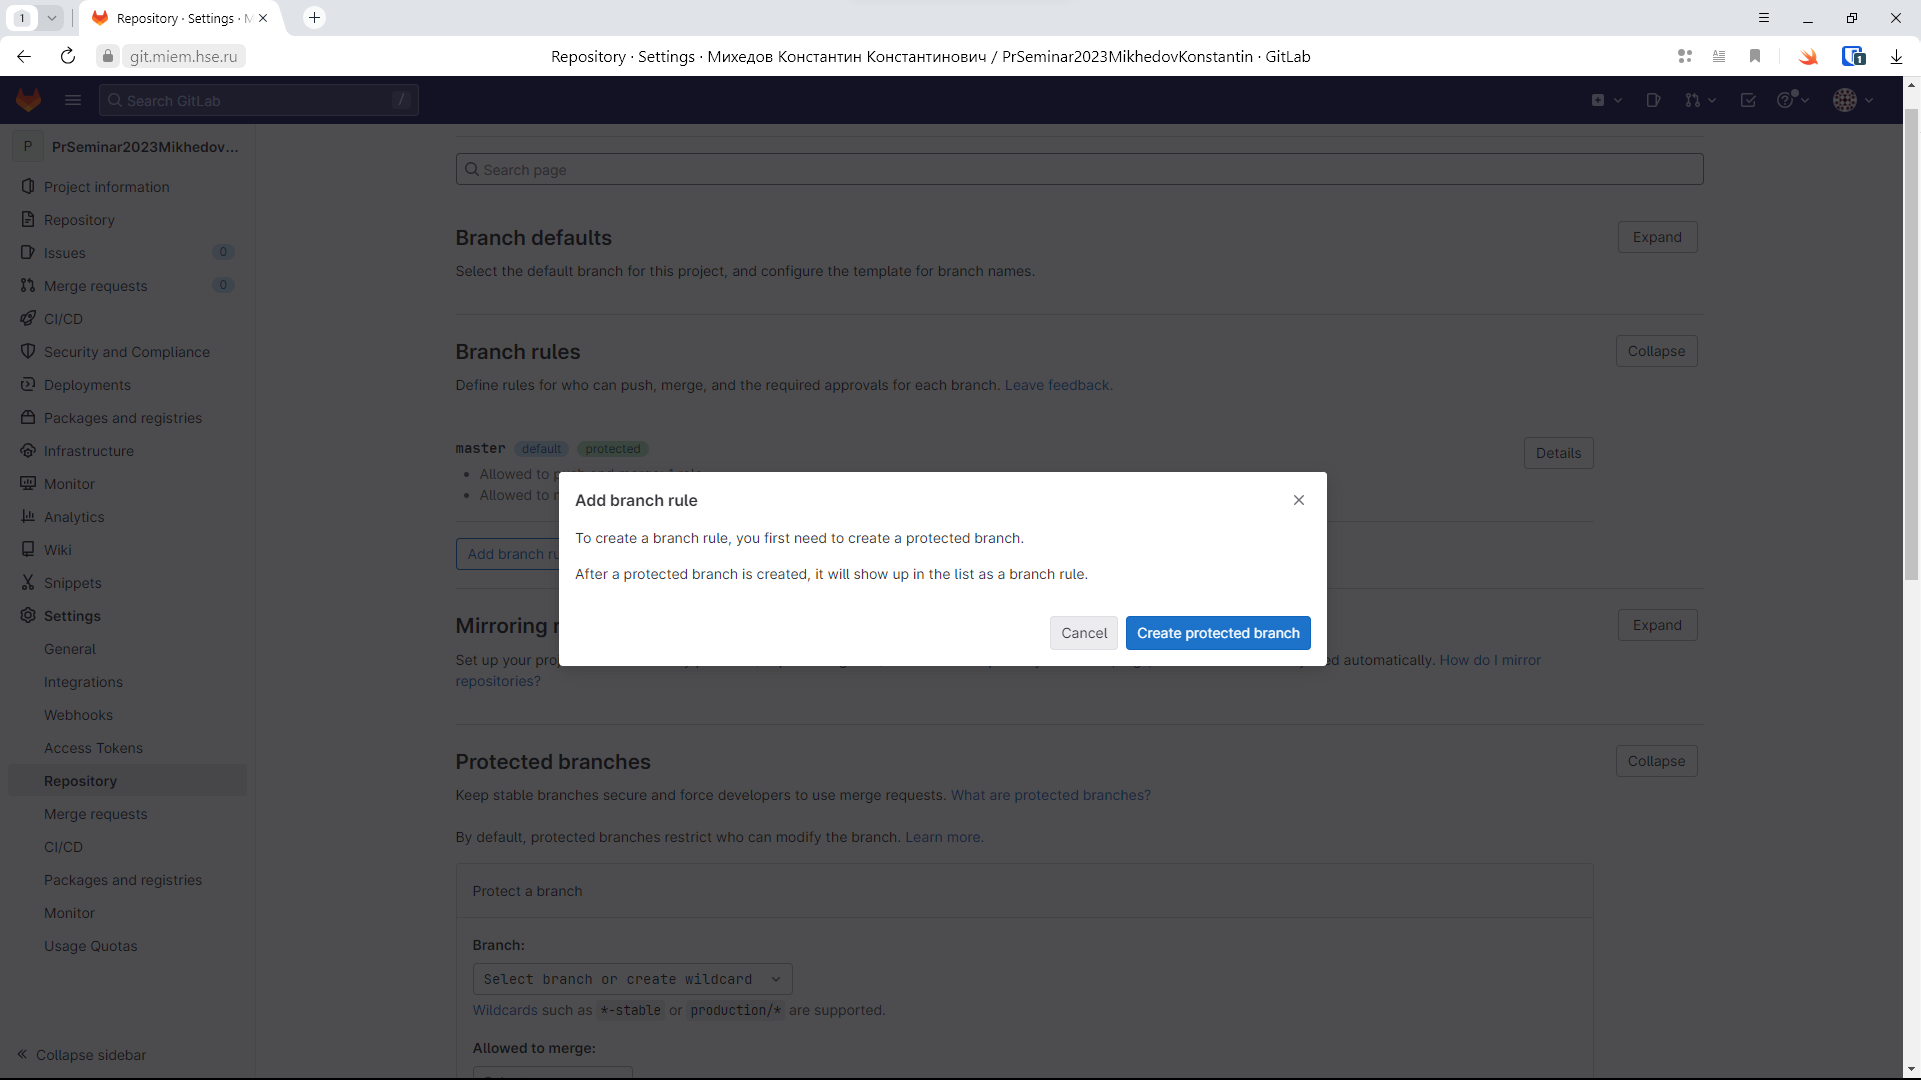
\includegraphics[width=\textwidth]{1_ (41)}
    \caption{Нажимаем кнопку <<Add branch rules>>, затем <<Create protected branch>>}
  \end{figure}

  \begin{figure}[H]
    \centering
    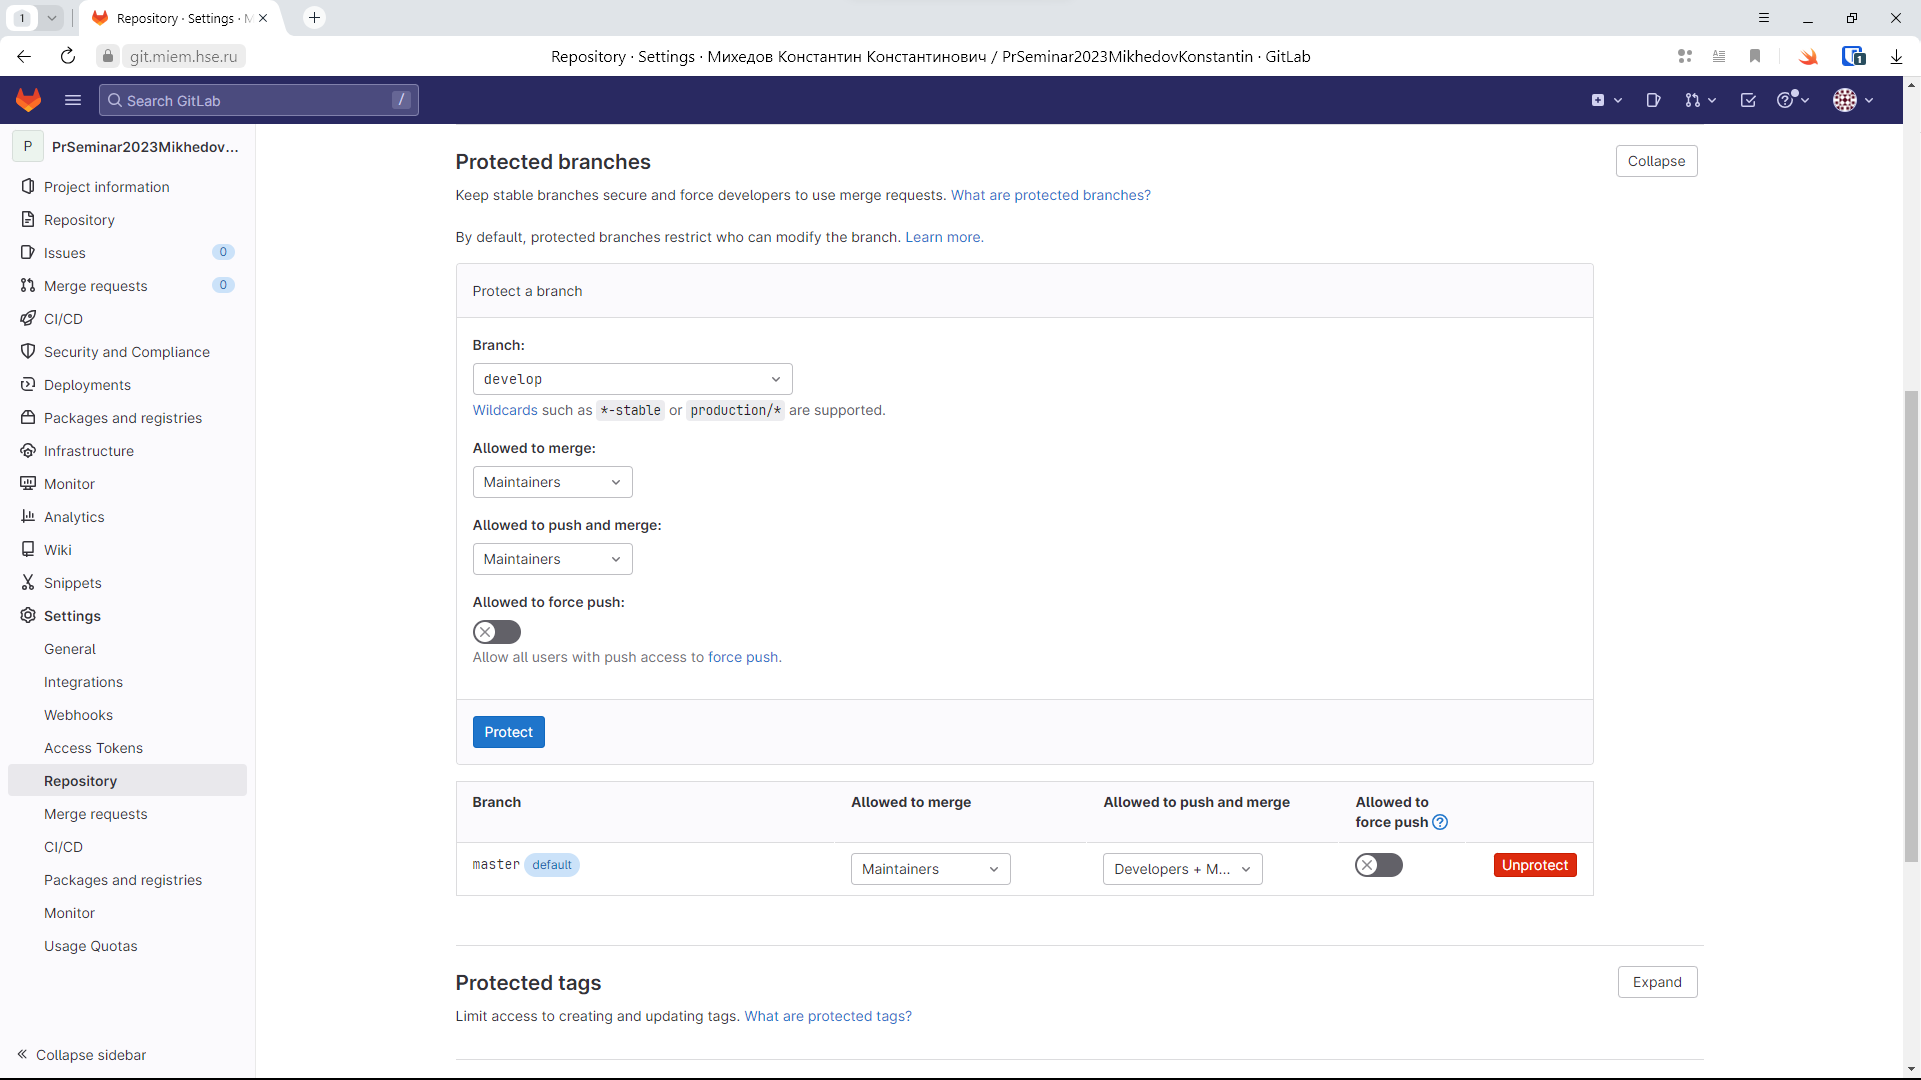
\includegraphics[width=\textwidth]{1_ (40)}
    \caption{Указываем ветку для внесения изменений и необходимые права}
  \end{figure}

  Здесь я добавил всем пользователям из группы maintainers возможность пушить и мерджить в ветку develop.
  По заданию для push операции нужно было полностью убрать доступ, я не заметил это при первом прочтении, поэтому это будет сделано позже.

  \begin{figure}[H]
    \centering
    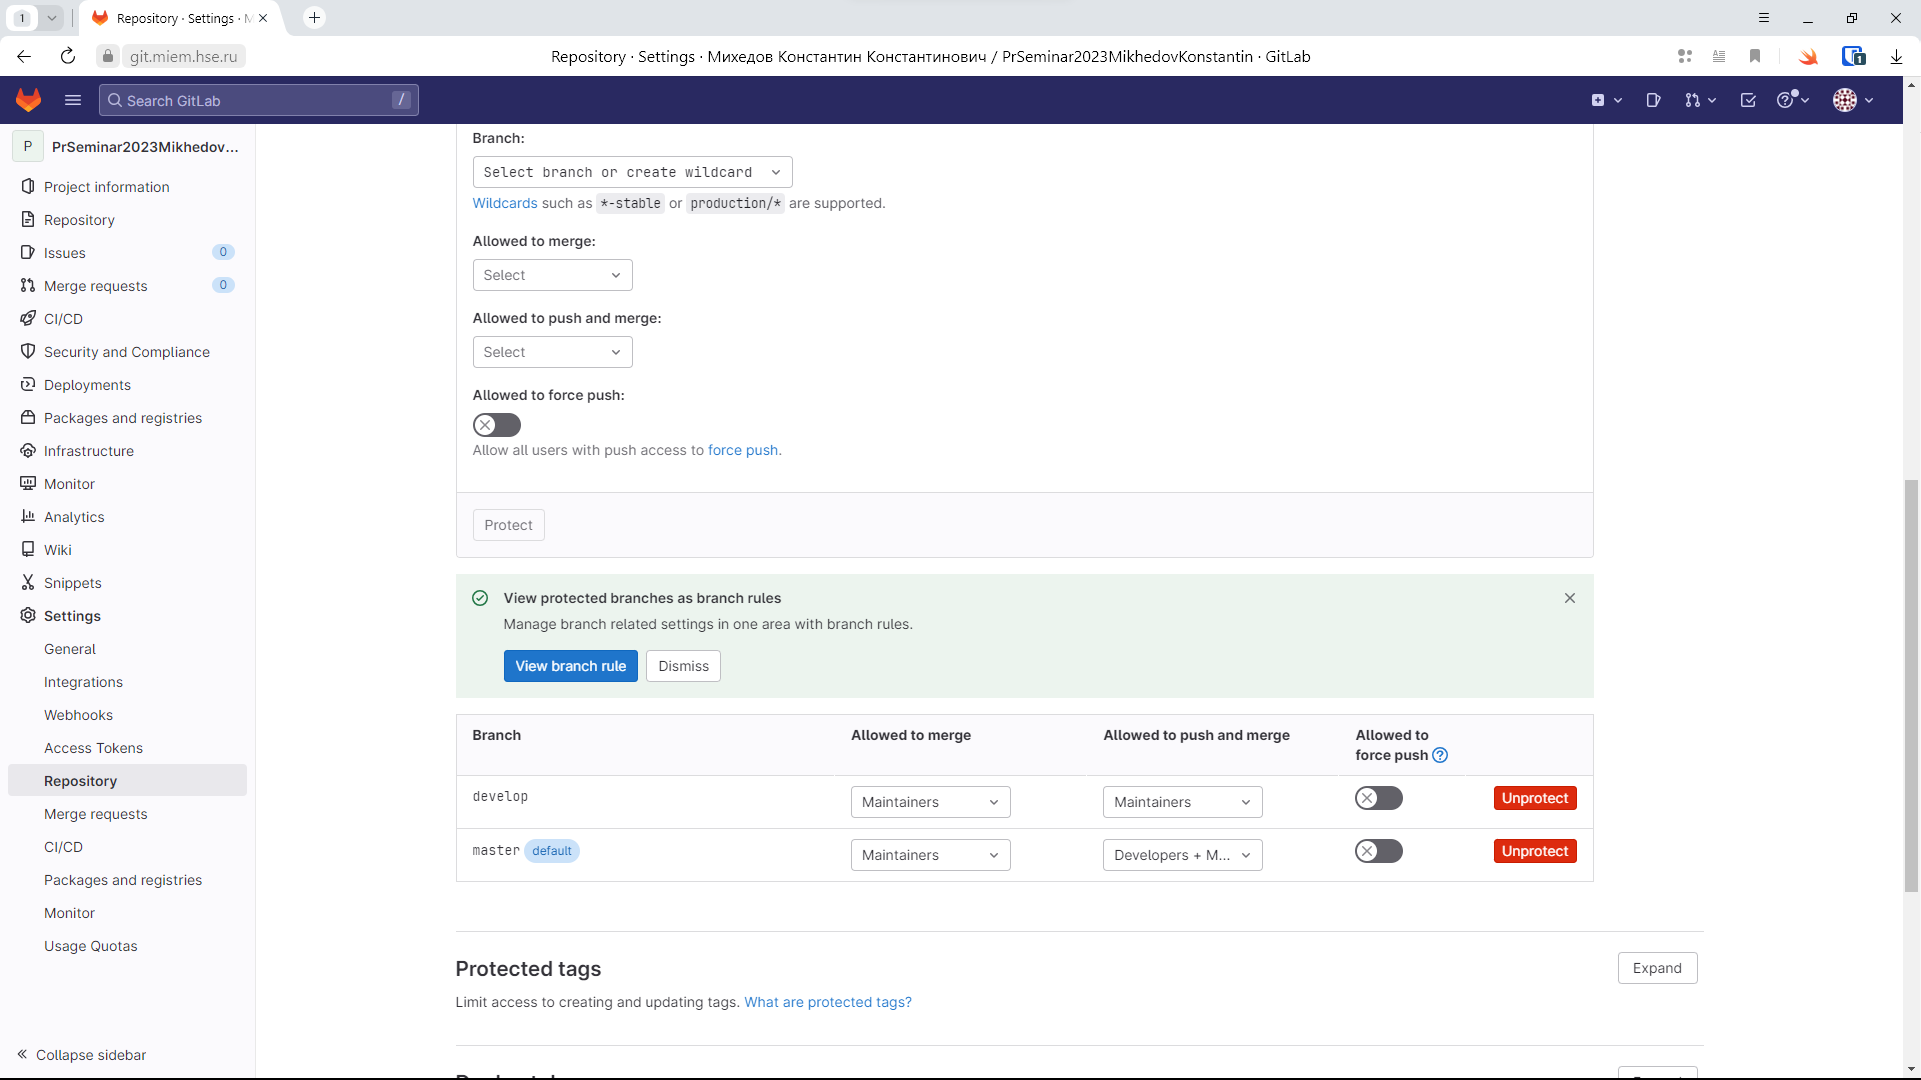
\includegraphics[width=\textwidth]{1_ (39)}
    \caption{Новая политика доступа появилась в списке}
  \end{figure}

  \begin{figure}[H]
    \centering
    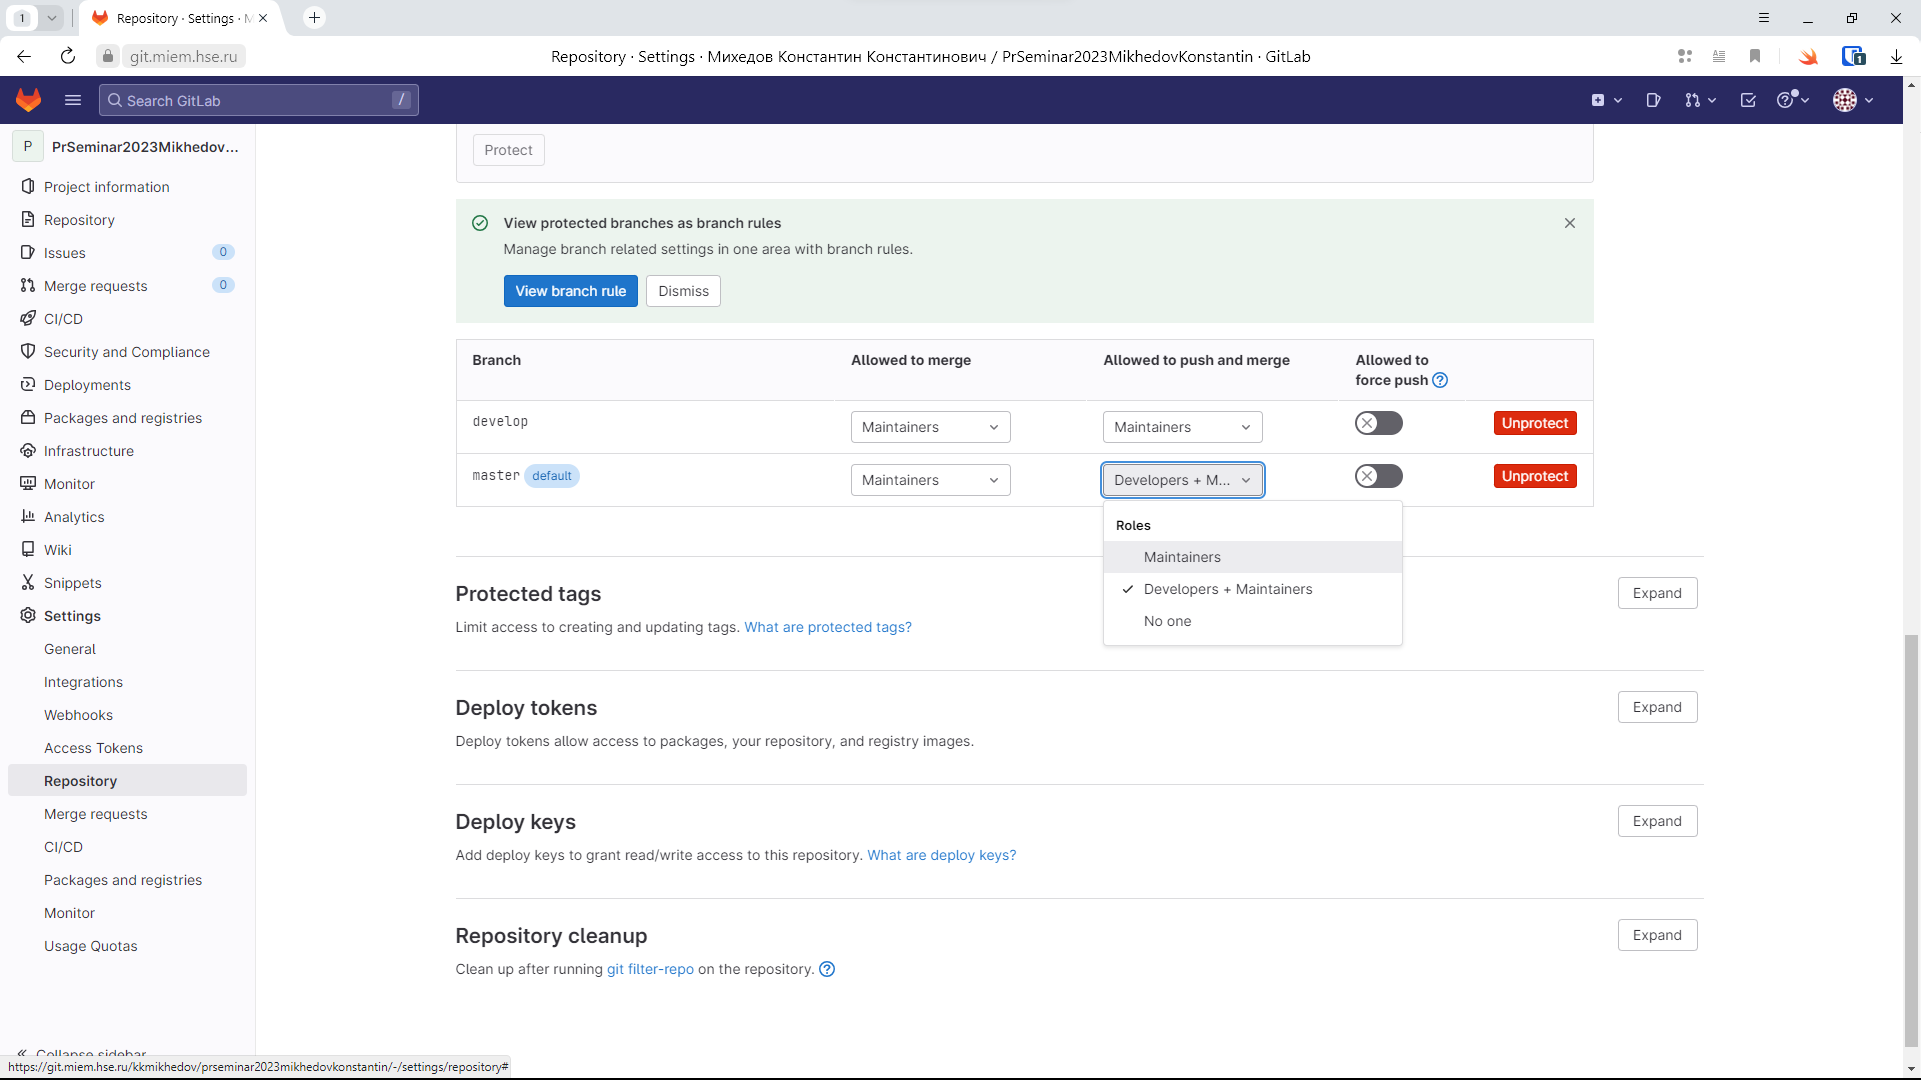
\includegraphics[width=\textwidth]{1_ (37)}
    \caption{Устанавливаем аналогичные права для master ветки}
  \end{figure}

  \begin{figure}[H]
    \centering
    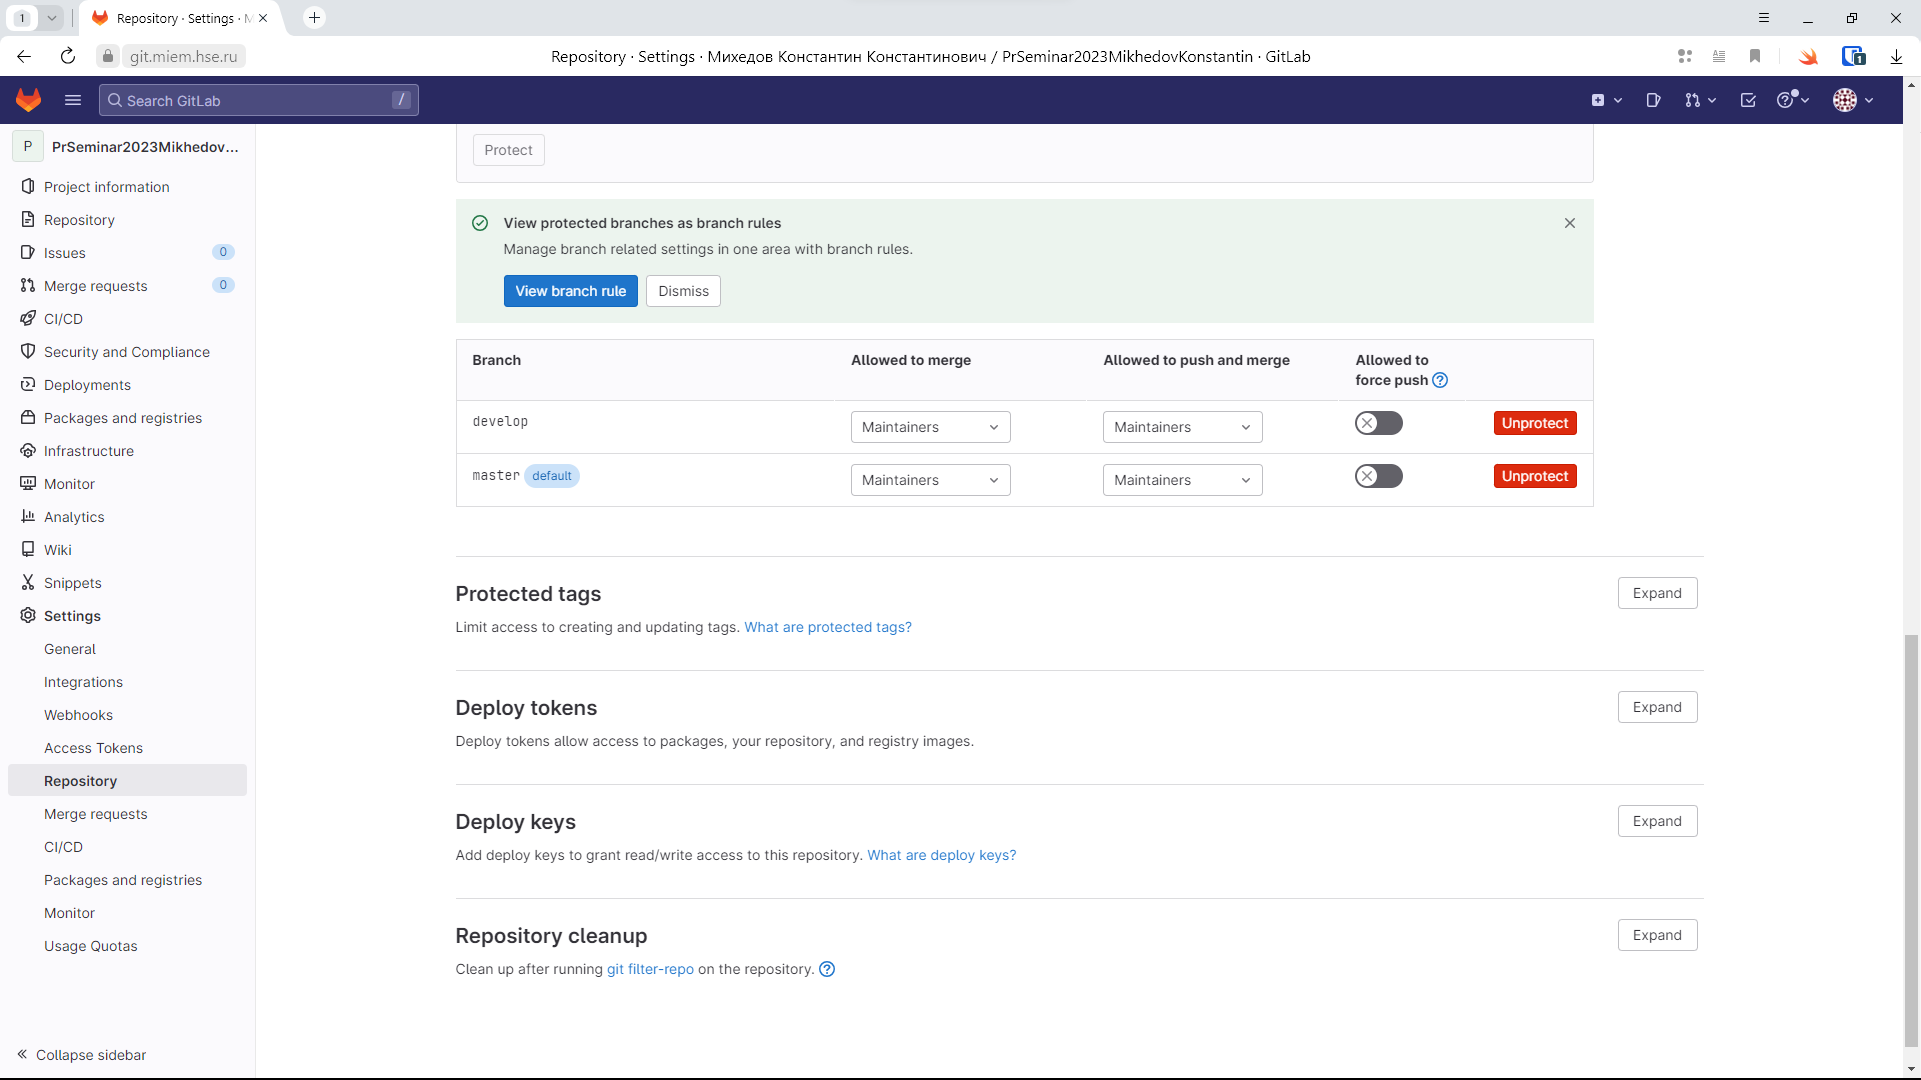
\includegraphics[width=\textwidth]{1_ (36)}
    \caption{Почти итоговые права для двух веток}
  \end{figure}

  \subsubsection{Настройка ветки по умолчанию}

  \begin{figure}[H]
    \centering
    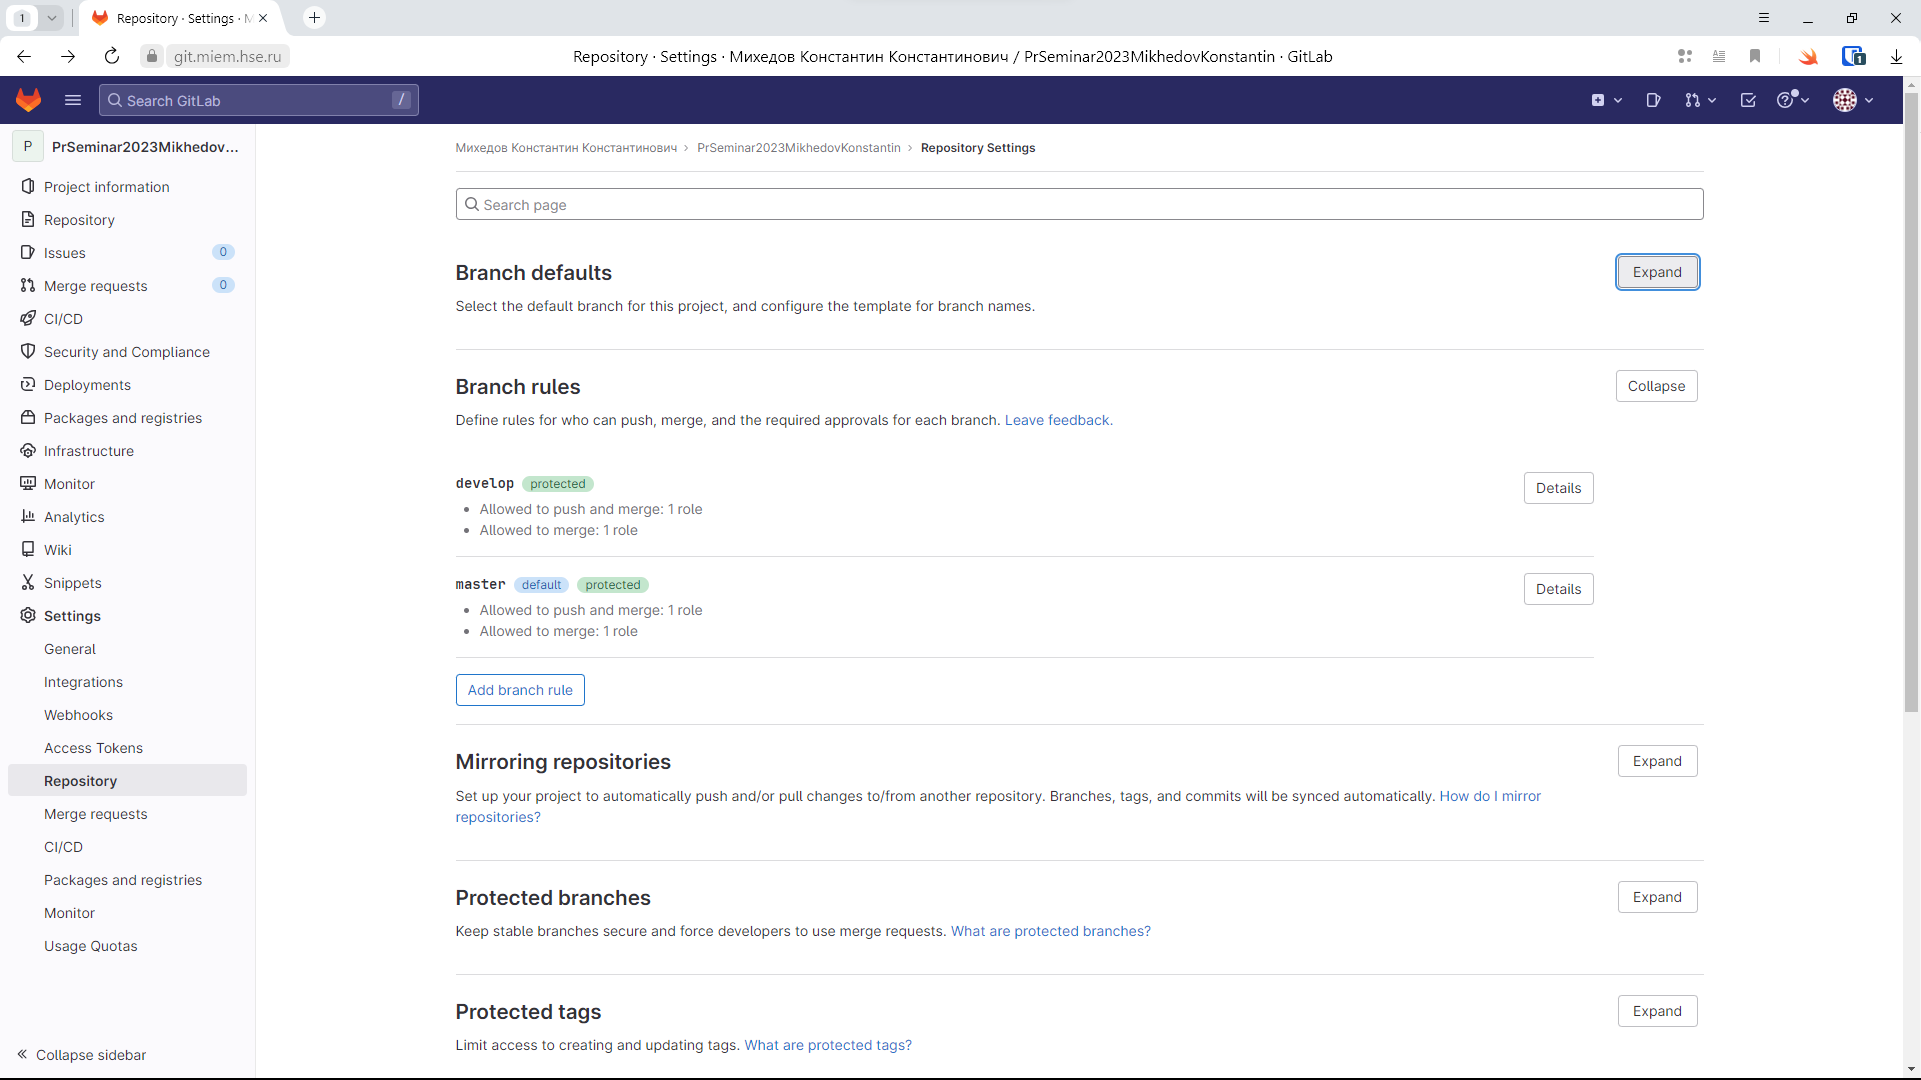
\includegraphics[width=\textwidth]{1_ (35)}
    \caption{Переходим к секции <<Branch defaults>>}
  \end{figure}

  \begin{figure}[H]
    \centering
    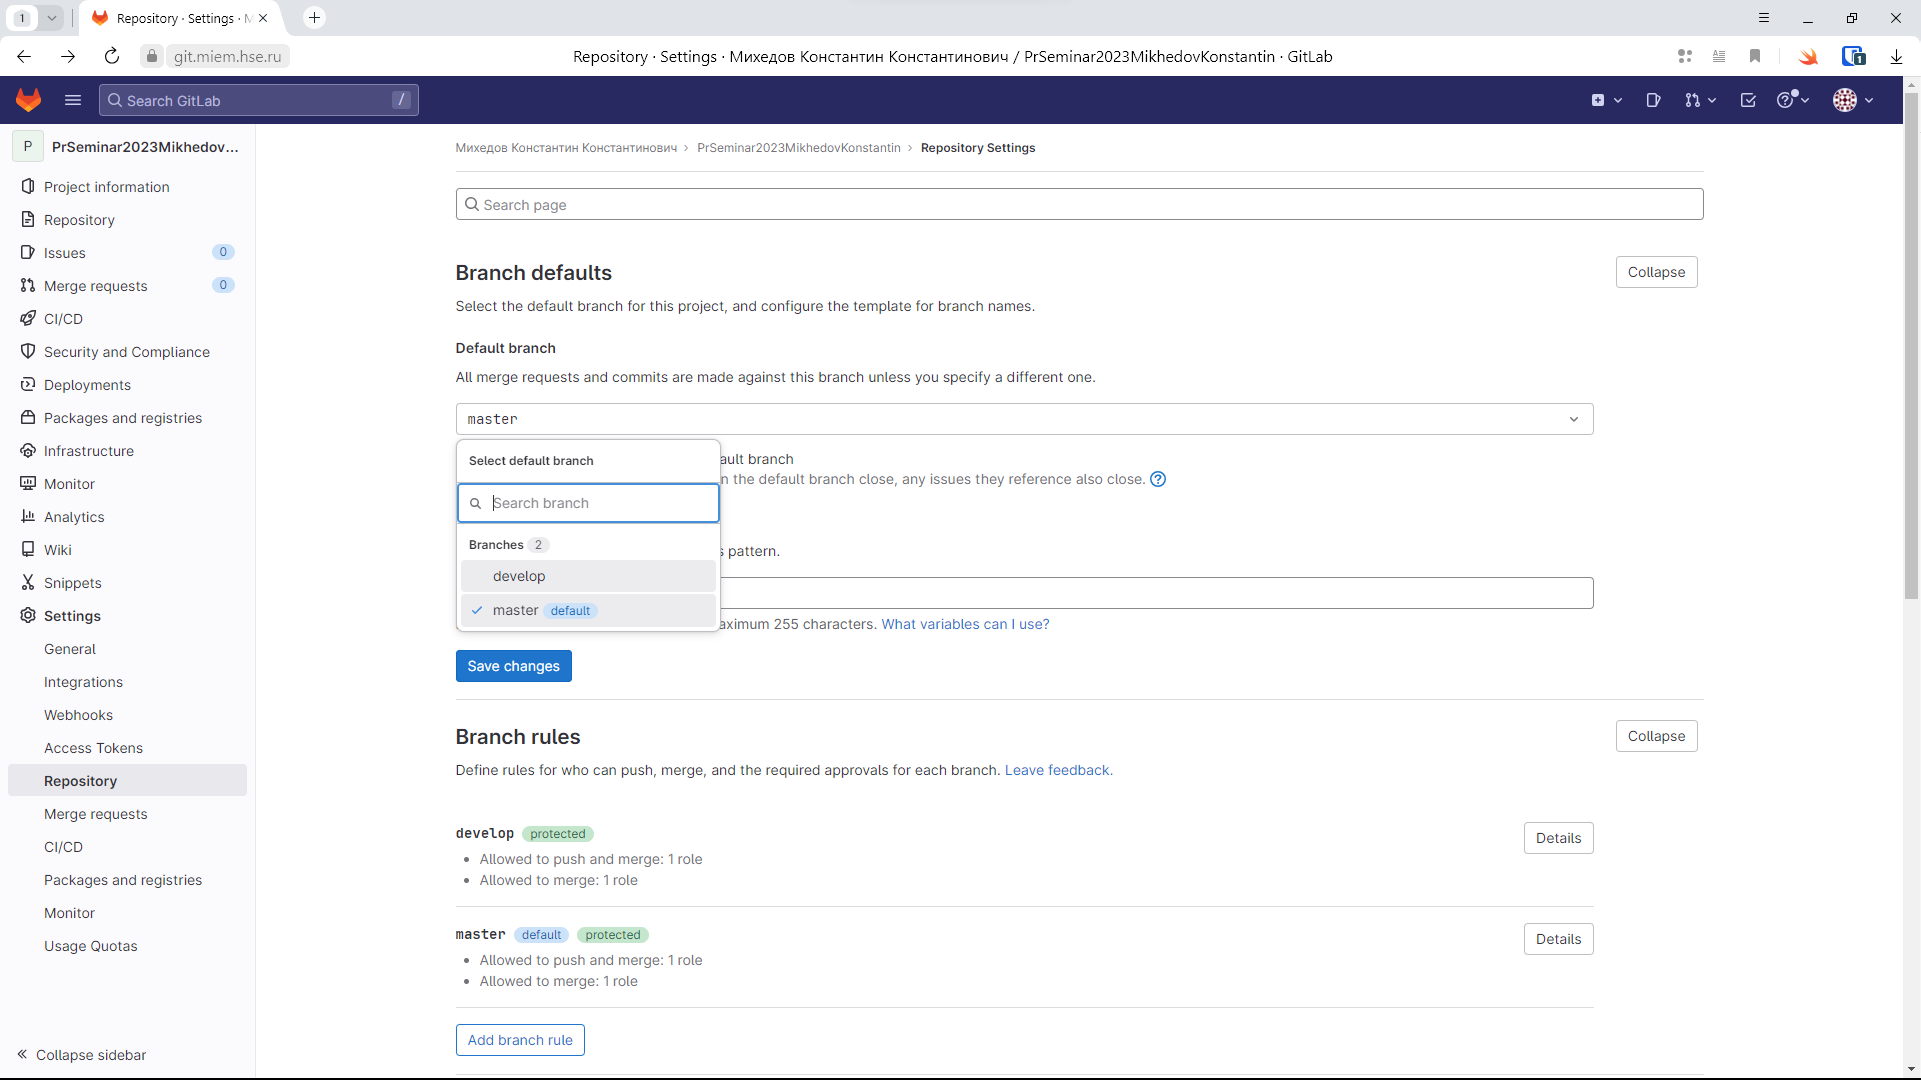
\includegraphics[width=\textwidth]{1_ (34)}
    \caption{Меняем ветку по умолчанию на develop}
  \end{figure}

  \begin{figure}[H]
    \centering
    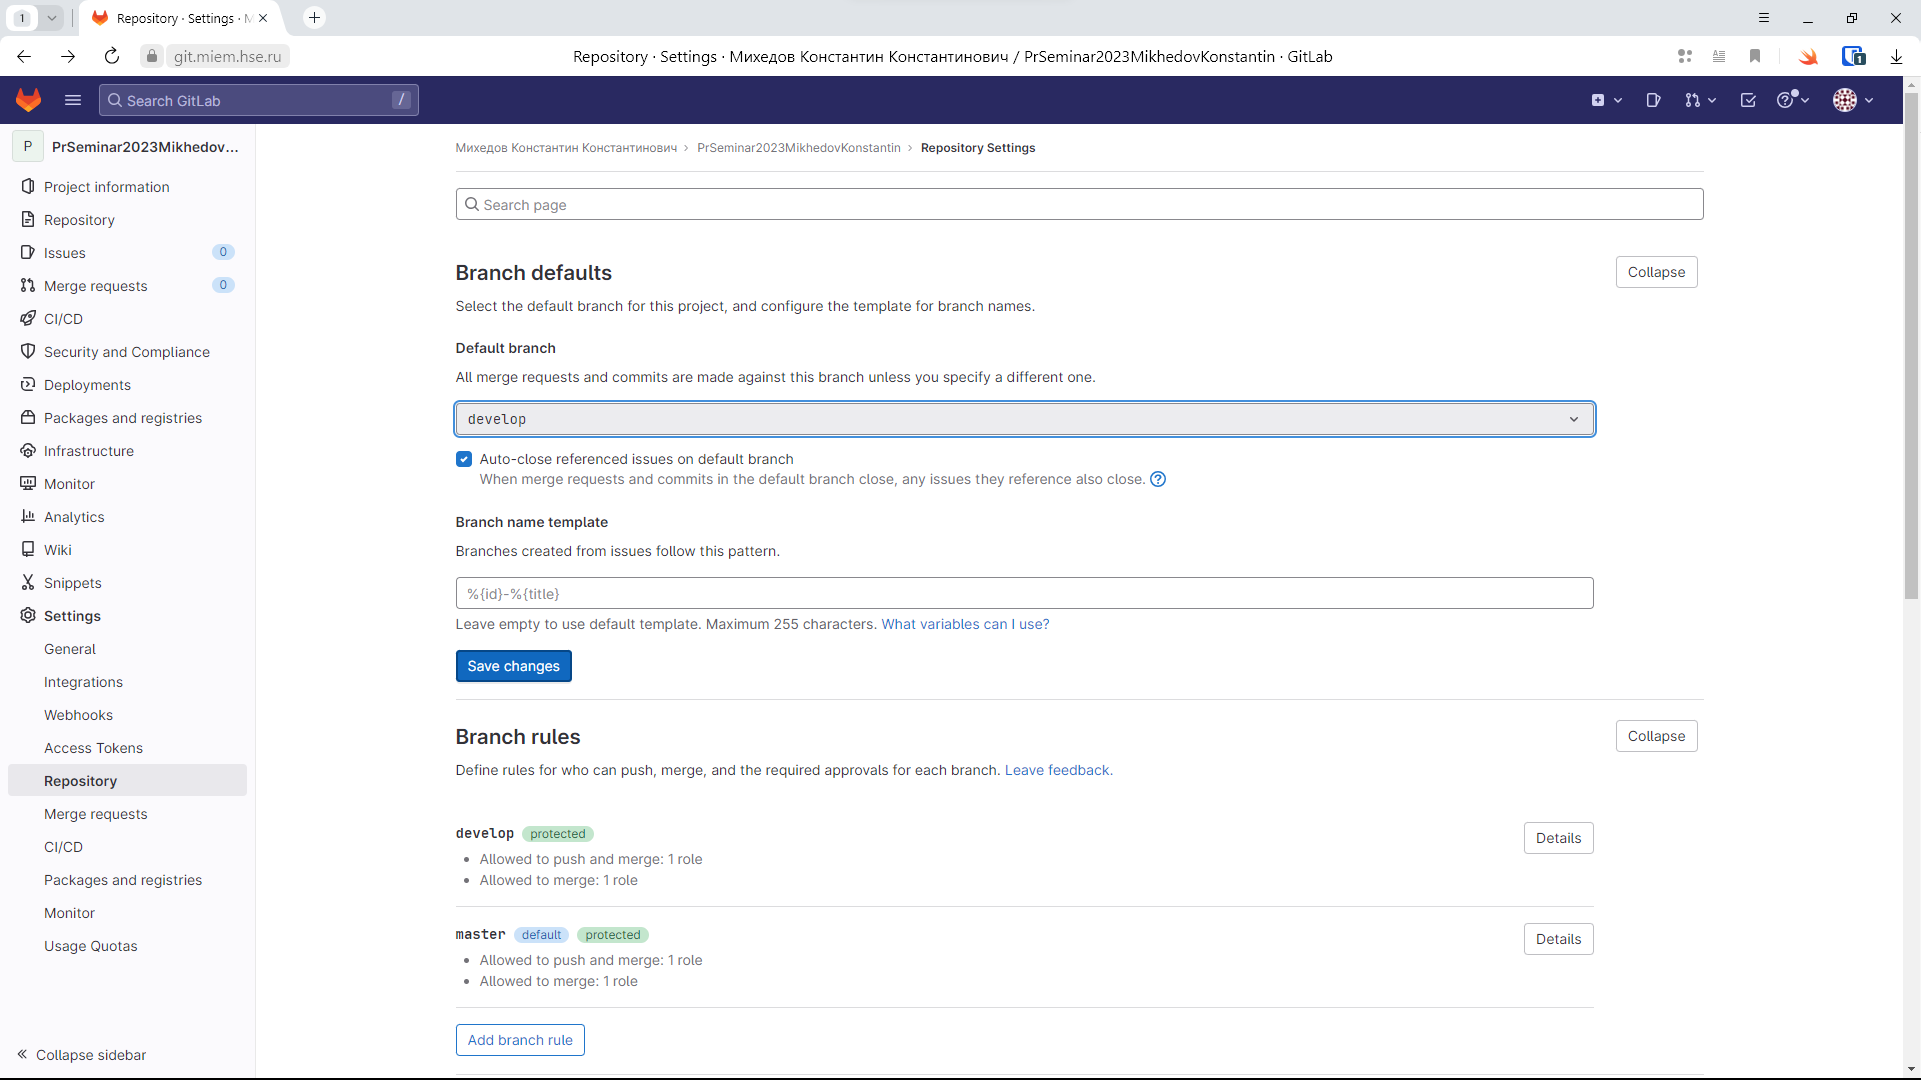
\includegraphics[width=\textwidth]{1_ (33)}
    \caption{Применяем изменения <<Save changes>>}
  \end{figure}

  \subsubsection{Настройка доступов. Попытка вторая}

  \begin{figure}[H]
    \centering
    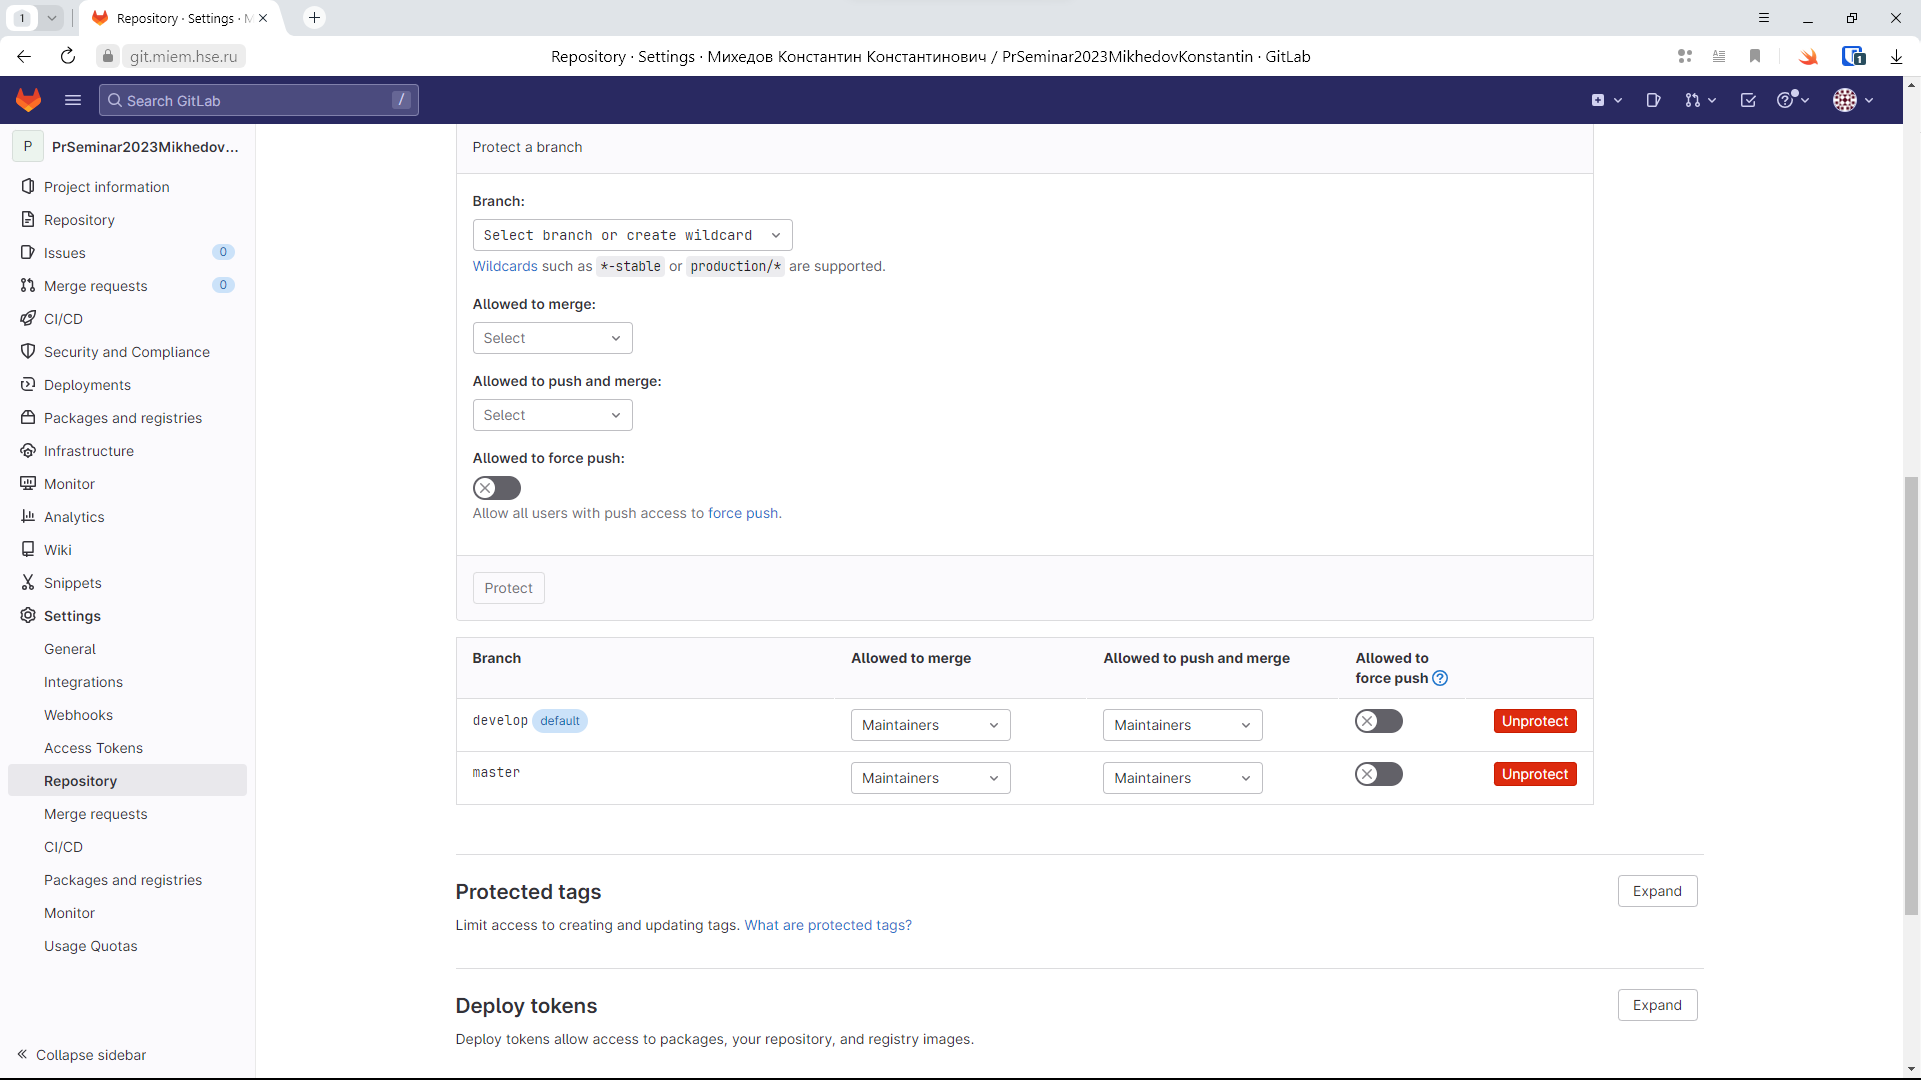
\includegraphics[width=\textwidth]{1_ (31)}
    \caption{Переходим к списку веток}
  \end{figure}

  \begin{figure}[H]
    \centering
    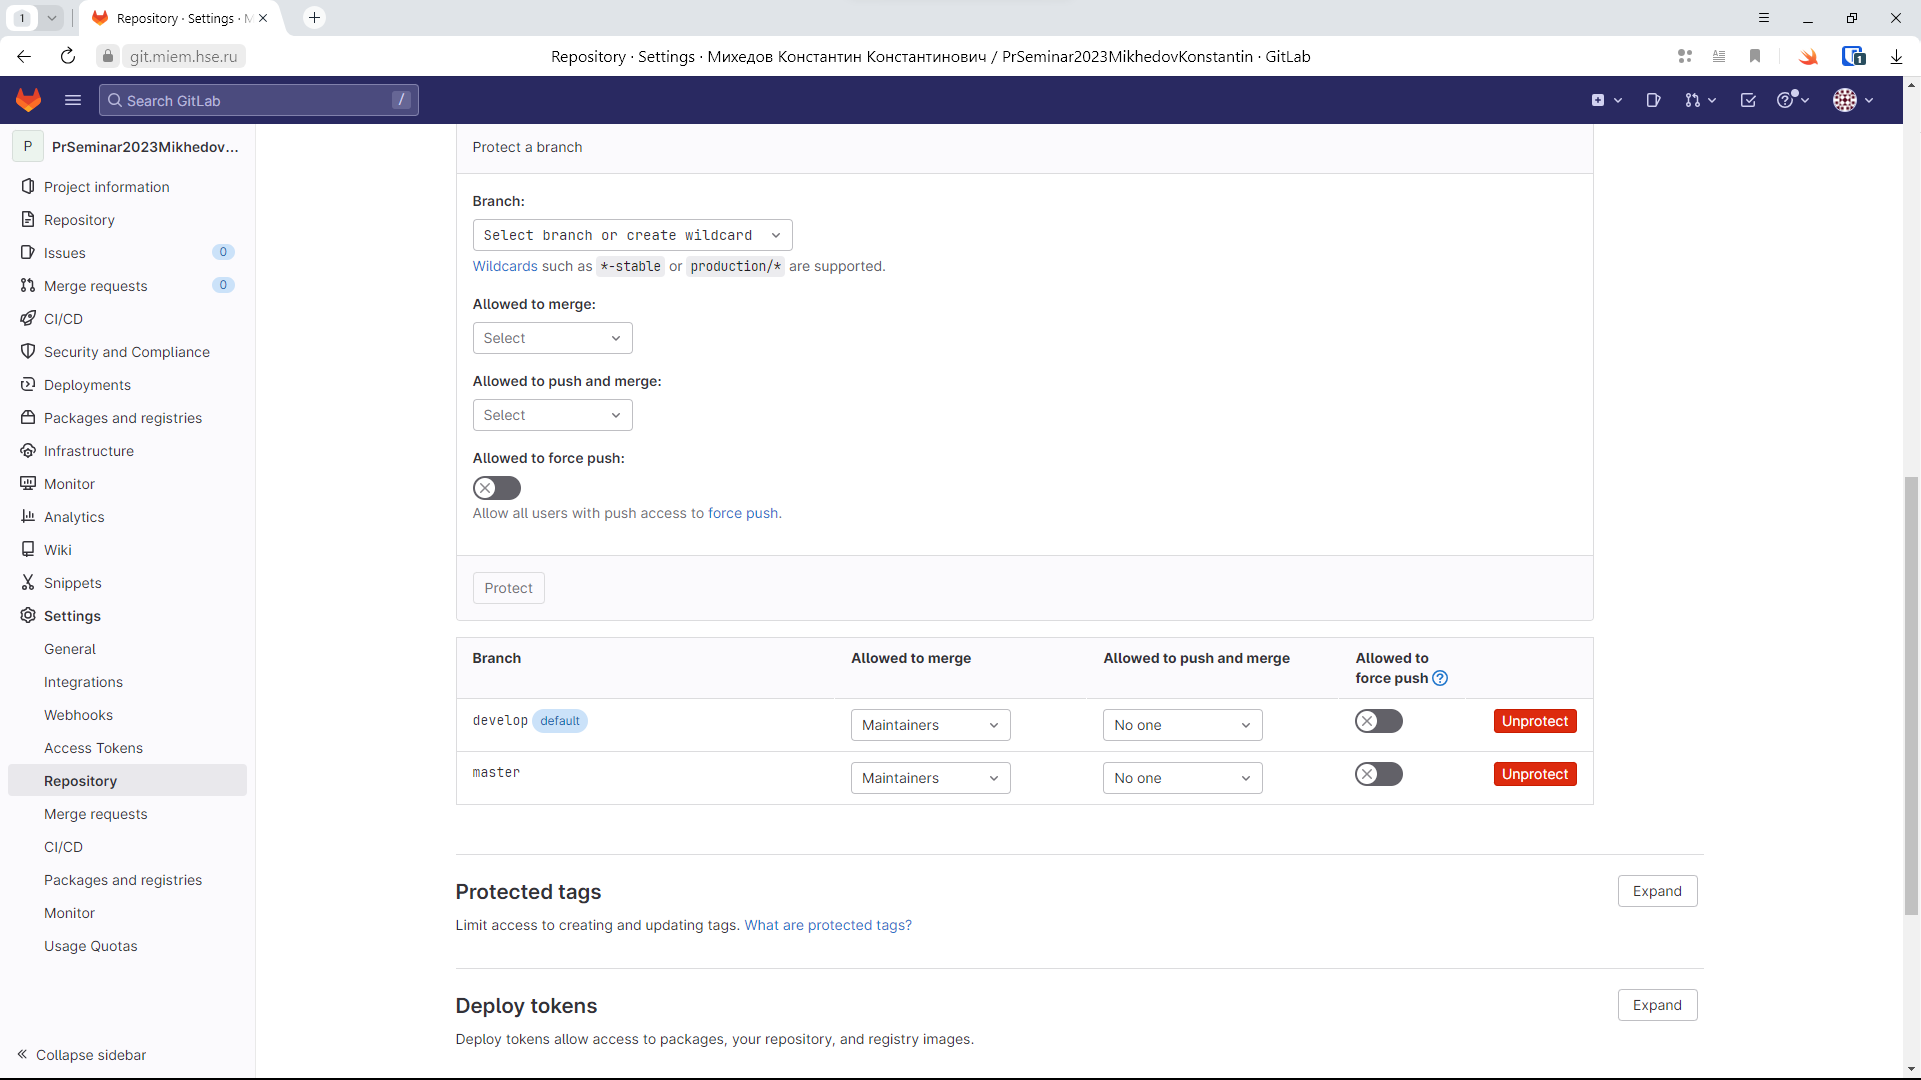
\includegraphics[width=\textwidth]{1_ (30)}
    \caption{Запрещаем push в обе ветки для всех}
  \end{figure}

  \subsubsection{Проверка политики}

  Пуш в ветку develop2 был запрещен, внесем изменения в локальную копию и попробуем
  отправить их в удаленный репозиторий:

  \begin{figure}[H]
    \centering
    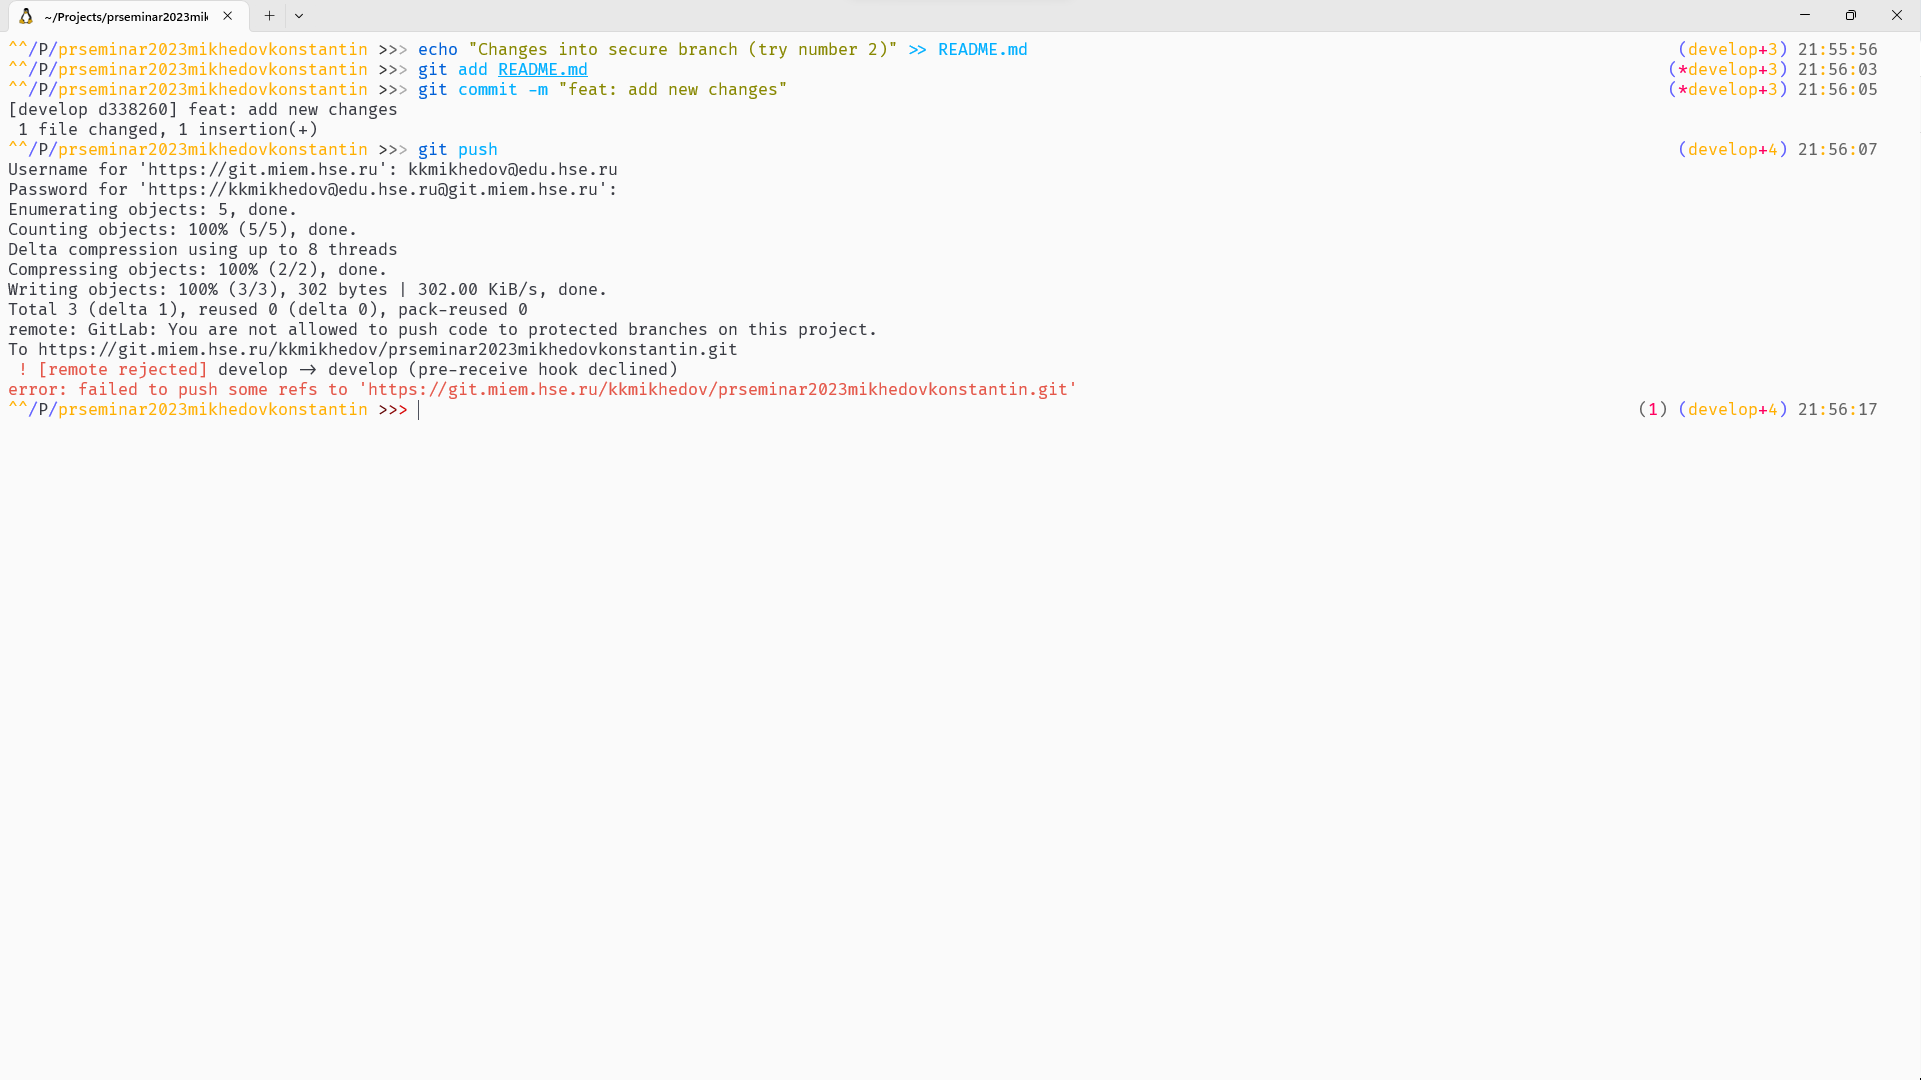
\includegraphics[width=\textwidth]{1_ (29)}
    \caption{Политика доступа отработала корректно}
  \end{figure}

  \begin{figure}[H]
    \centering
    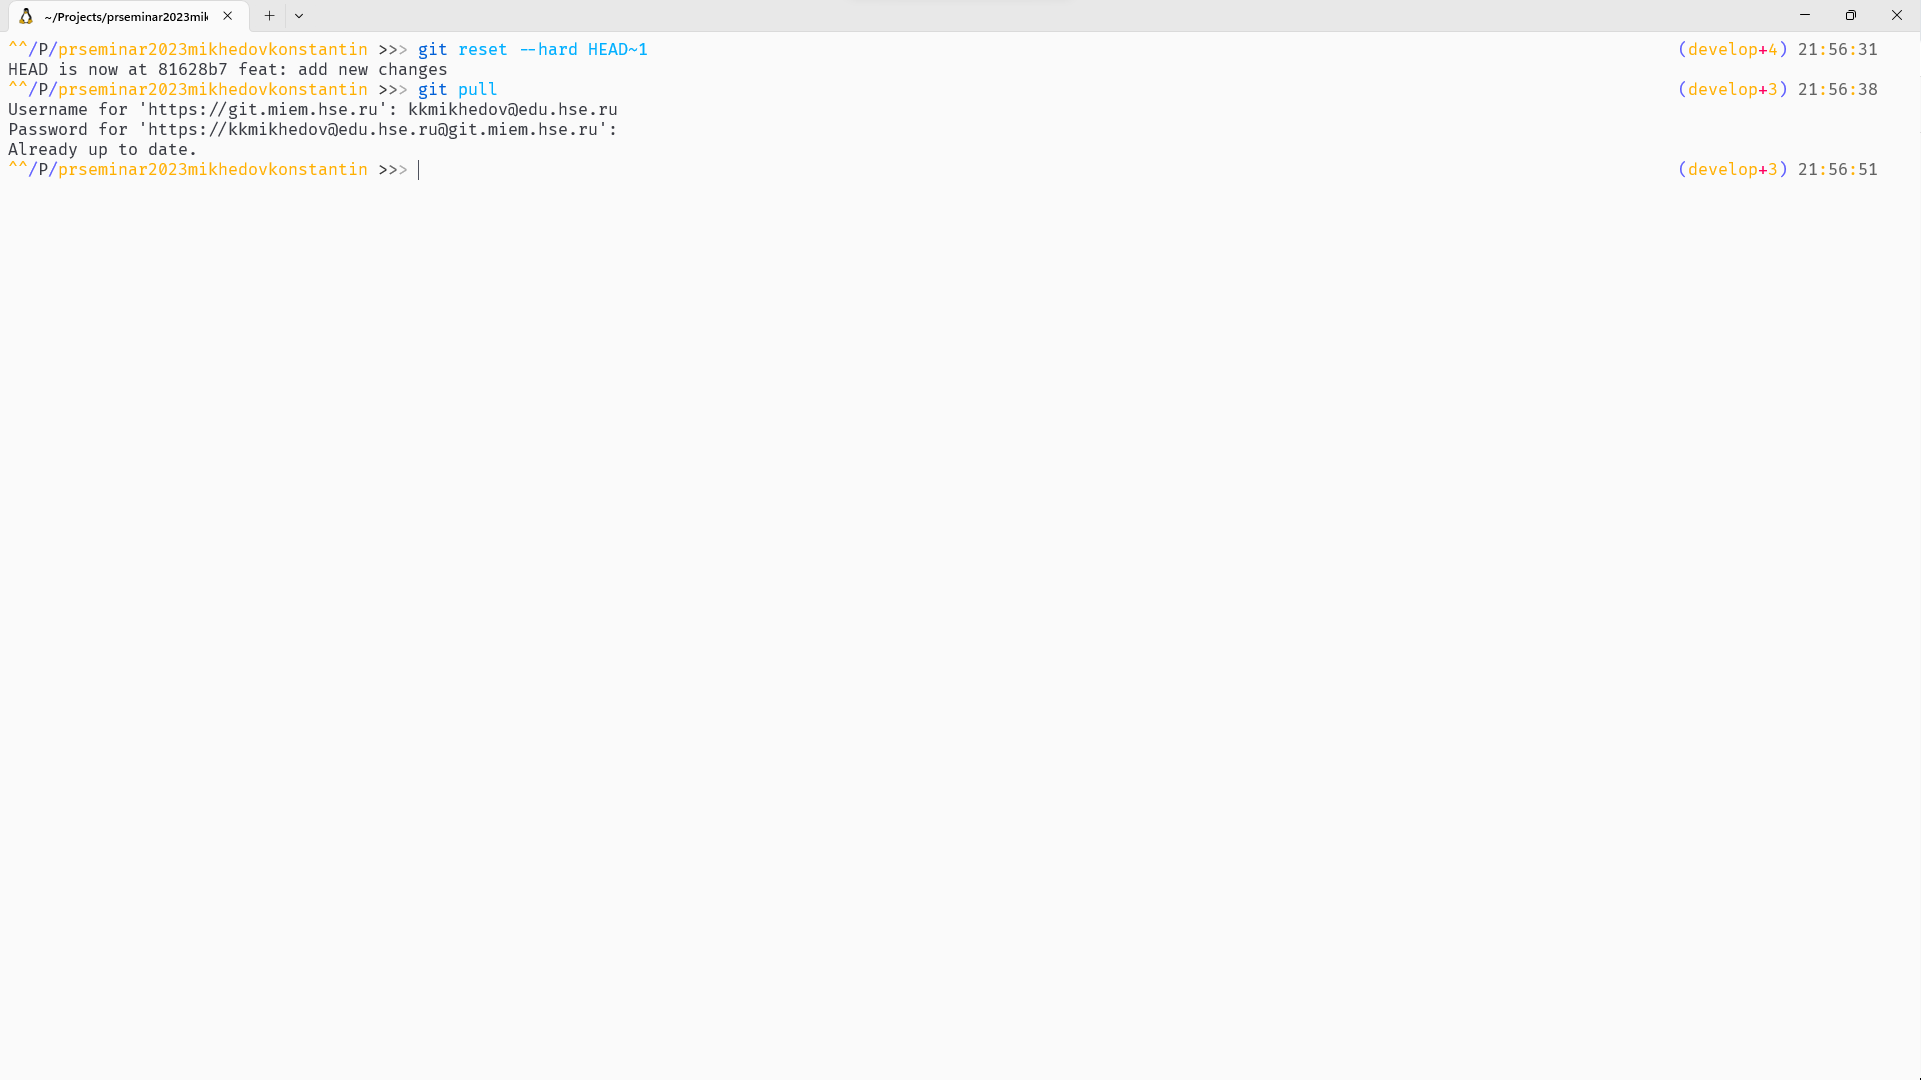
\includegraphics[width=\textwidth]{1_ (28)}
    \caption{Синхронизируем локальную копию с удаленном - отменим последний коммит и сделаем git pull}
  \end{figure}

  \subsection{Разрешение конфликтов}

  \begin{figure}[H]
    \centering
    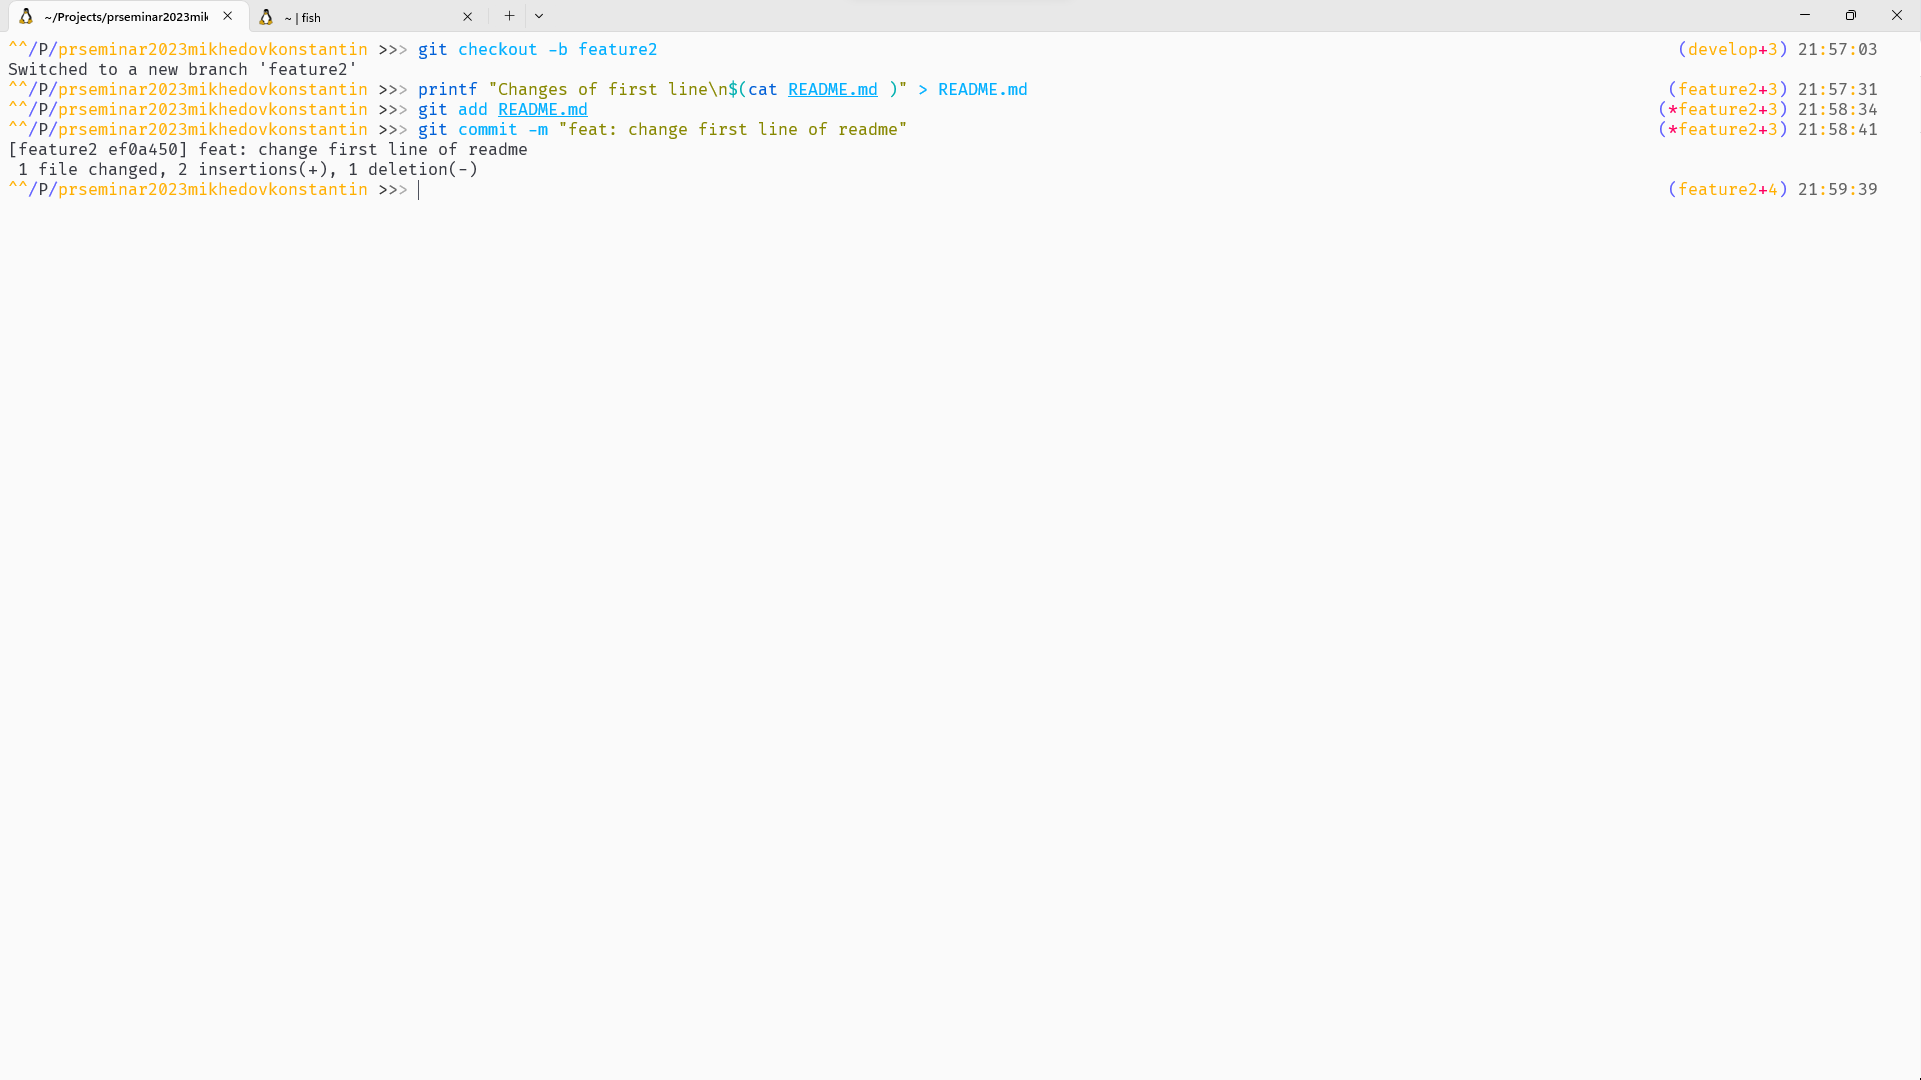
\includegraphics[width=\textwidth]{1_ (27)}
    \caption{Создадим ветку feature2 и внесем изменения в первую строку README.md, сделаем коммит}
  \end{figure}

  \begin{figure}[H]
    \centering
    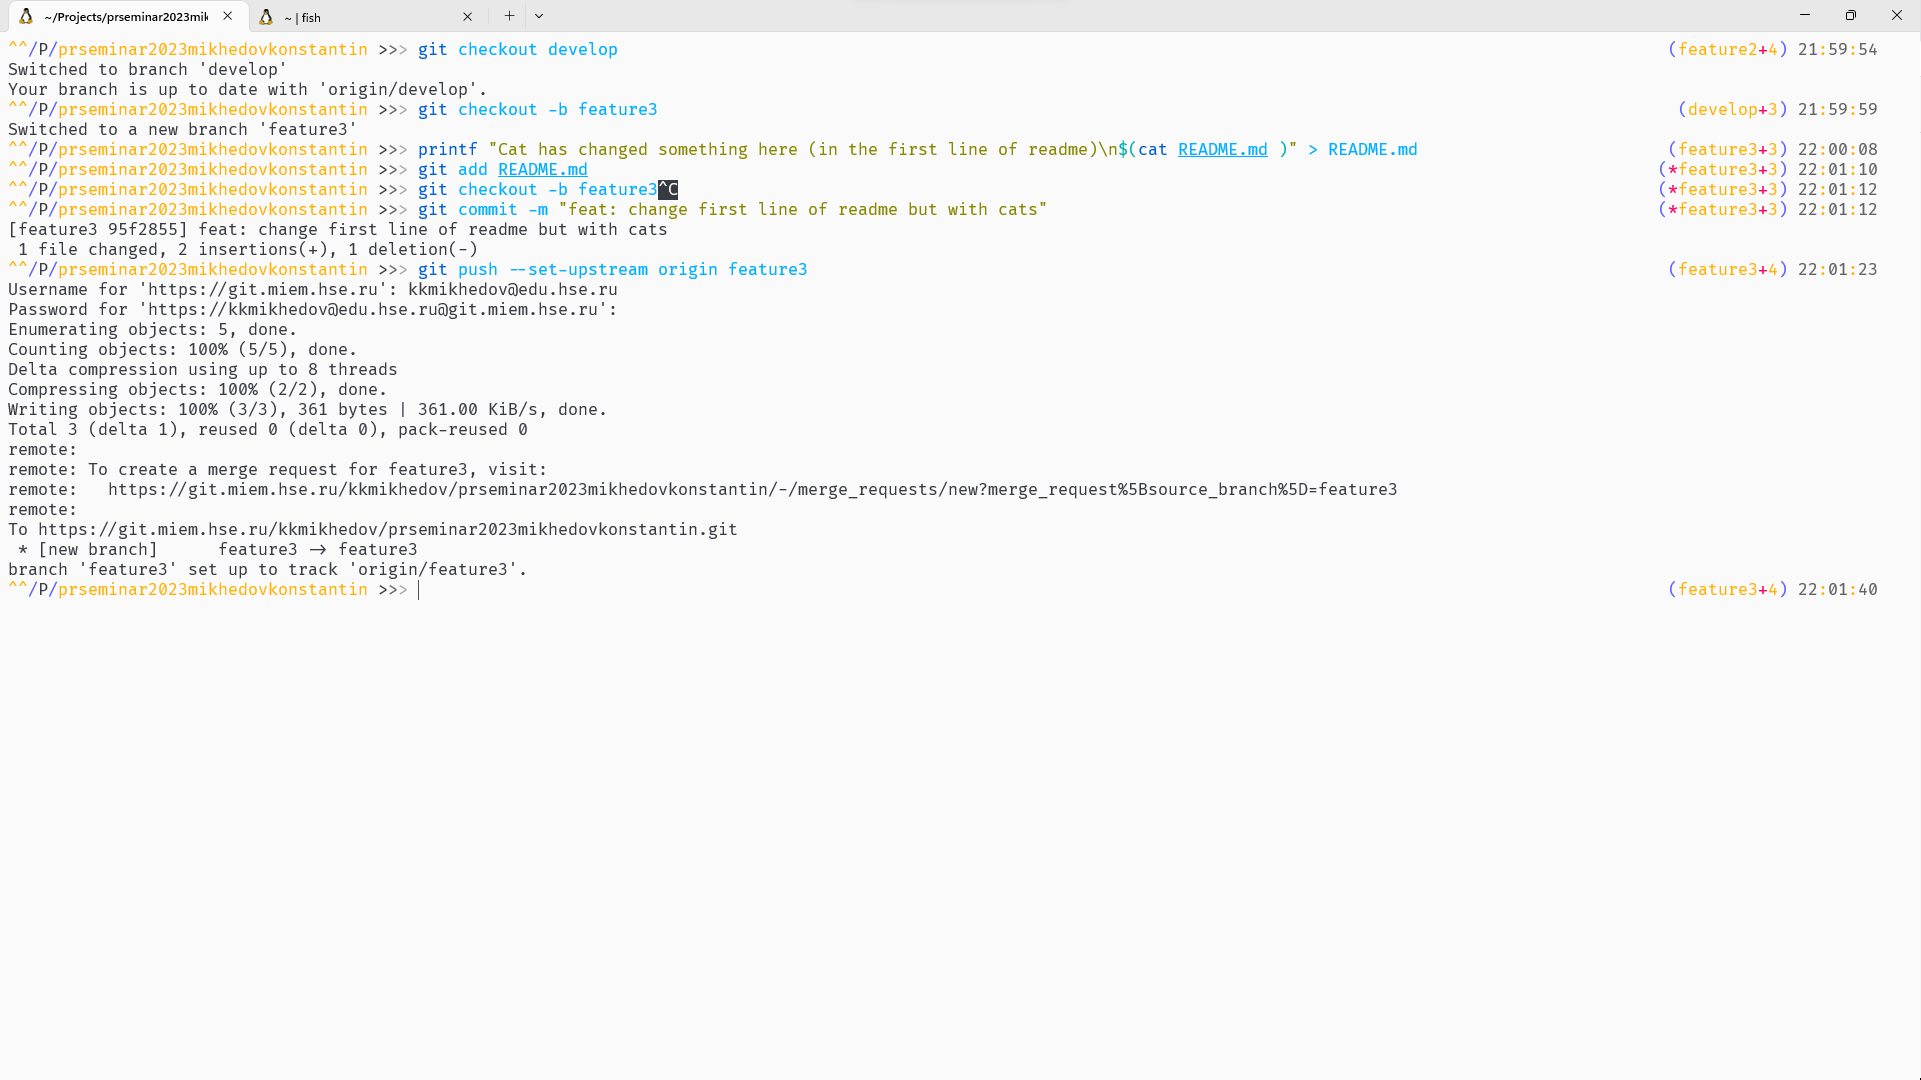
\includegraphics[width=\textwidth]{1_ (26)}
    \caption{Создадим ветку feature3, внесем изменения в первую строку README.md, сделаем коммит и отправим изменения на удаленный сервер}
  \end{figure}

  \begin{figure}[H]
    \centering
    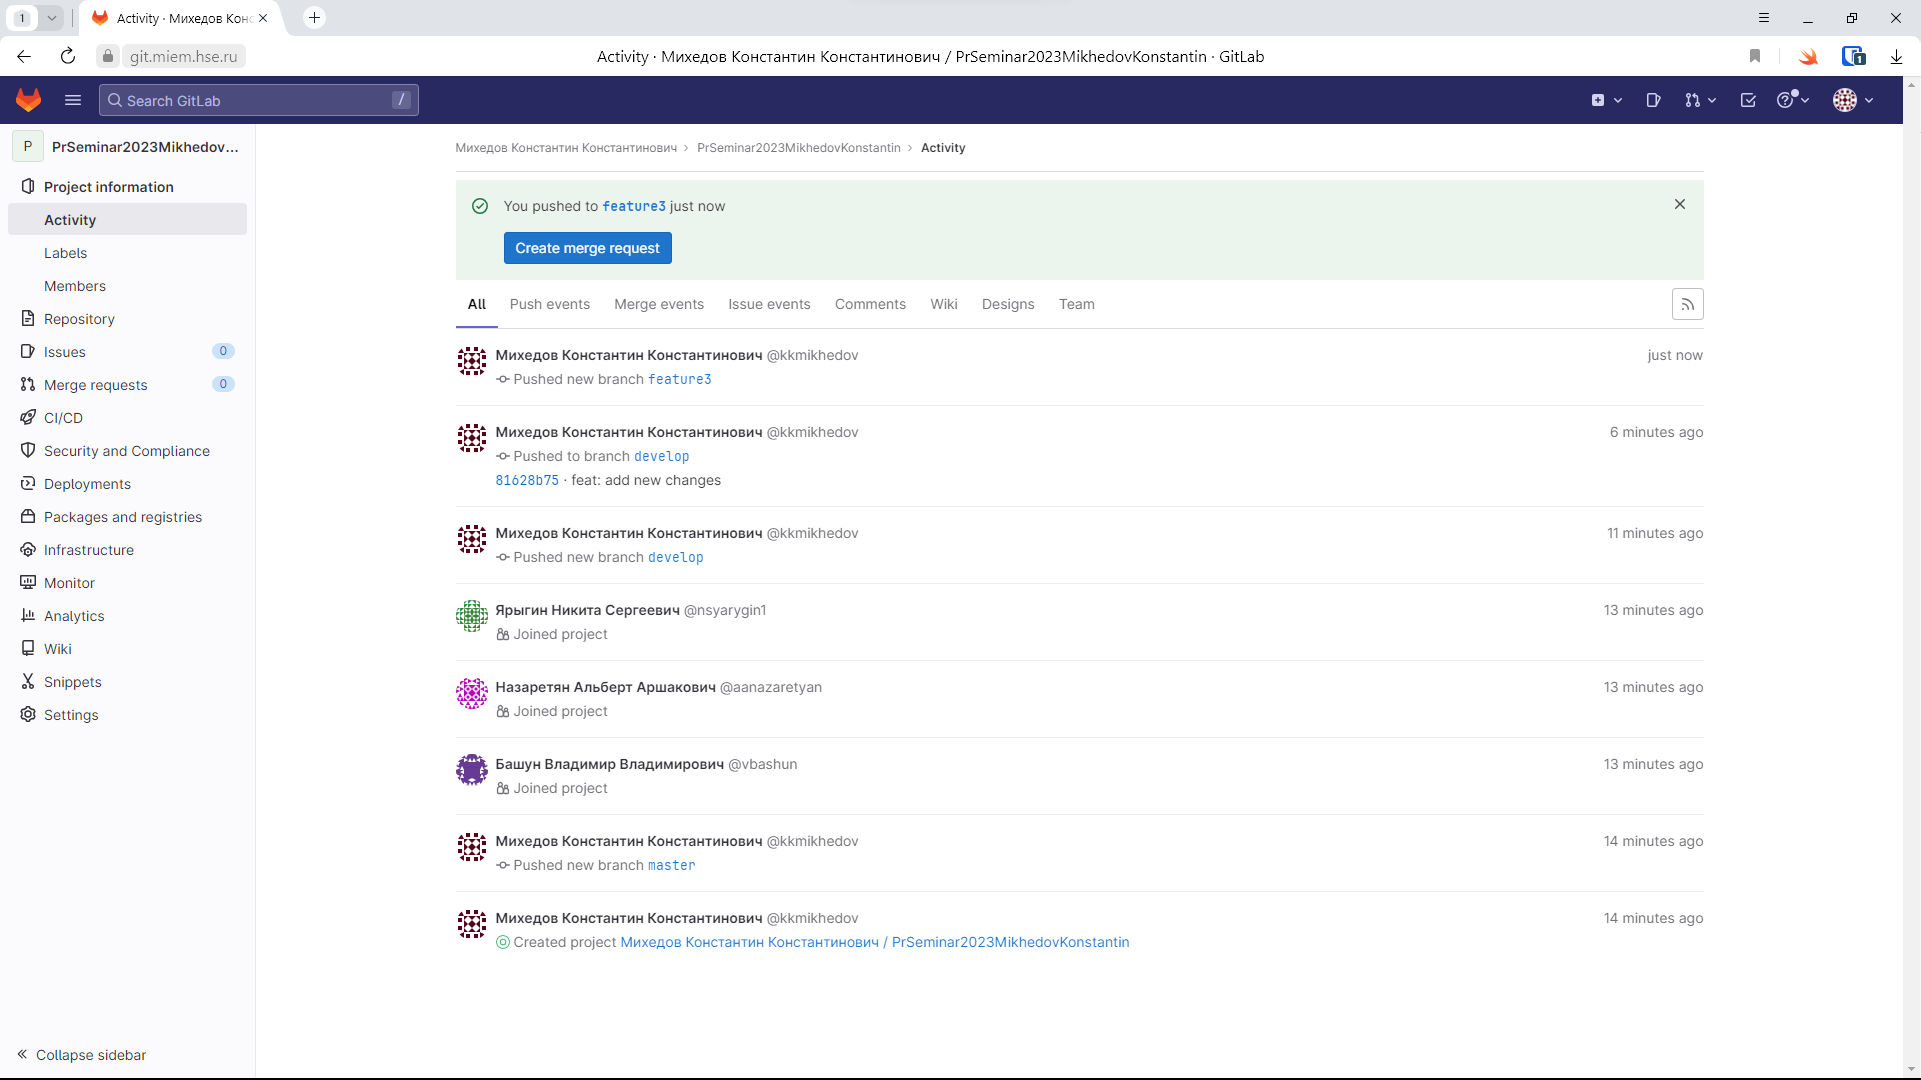
\includegraphics[width=\textwidth]{1_ (25)}
    \caption{feature3 ветка появилась в интерфейсе}
  \end{figure}

  \begin{figure}[H]
    \centering
    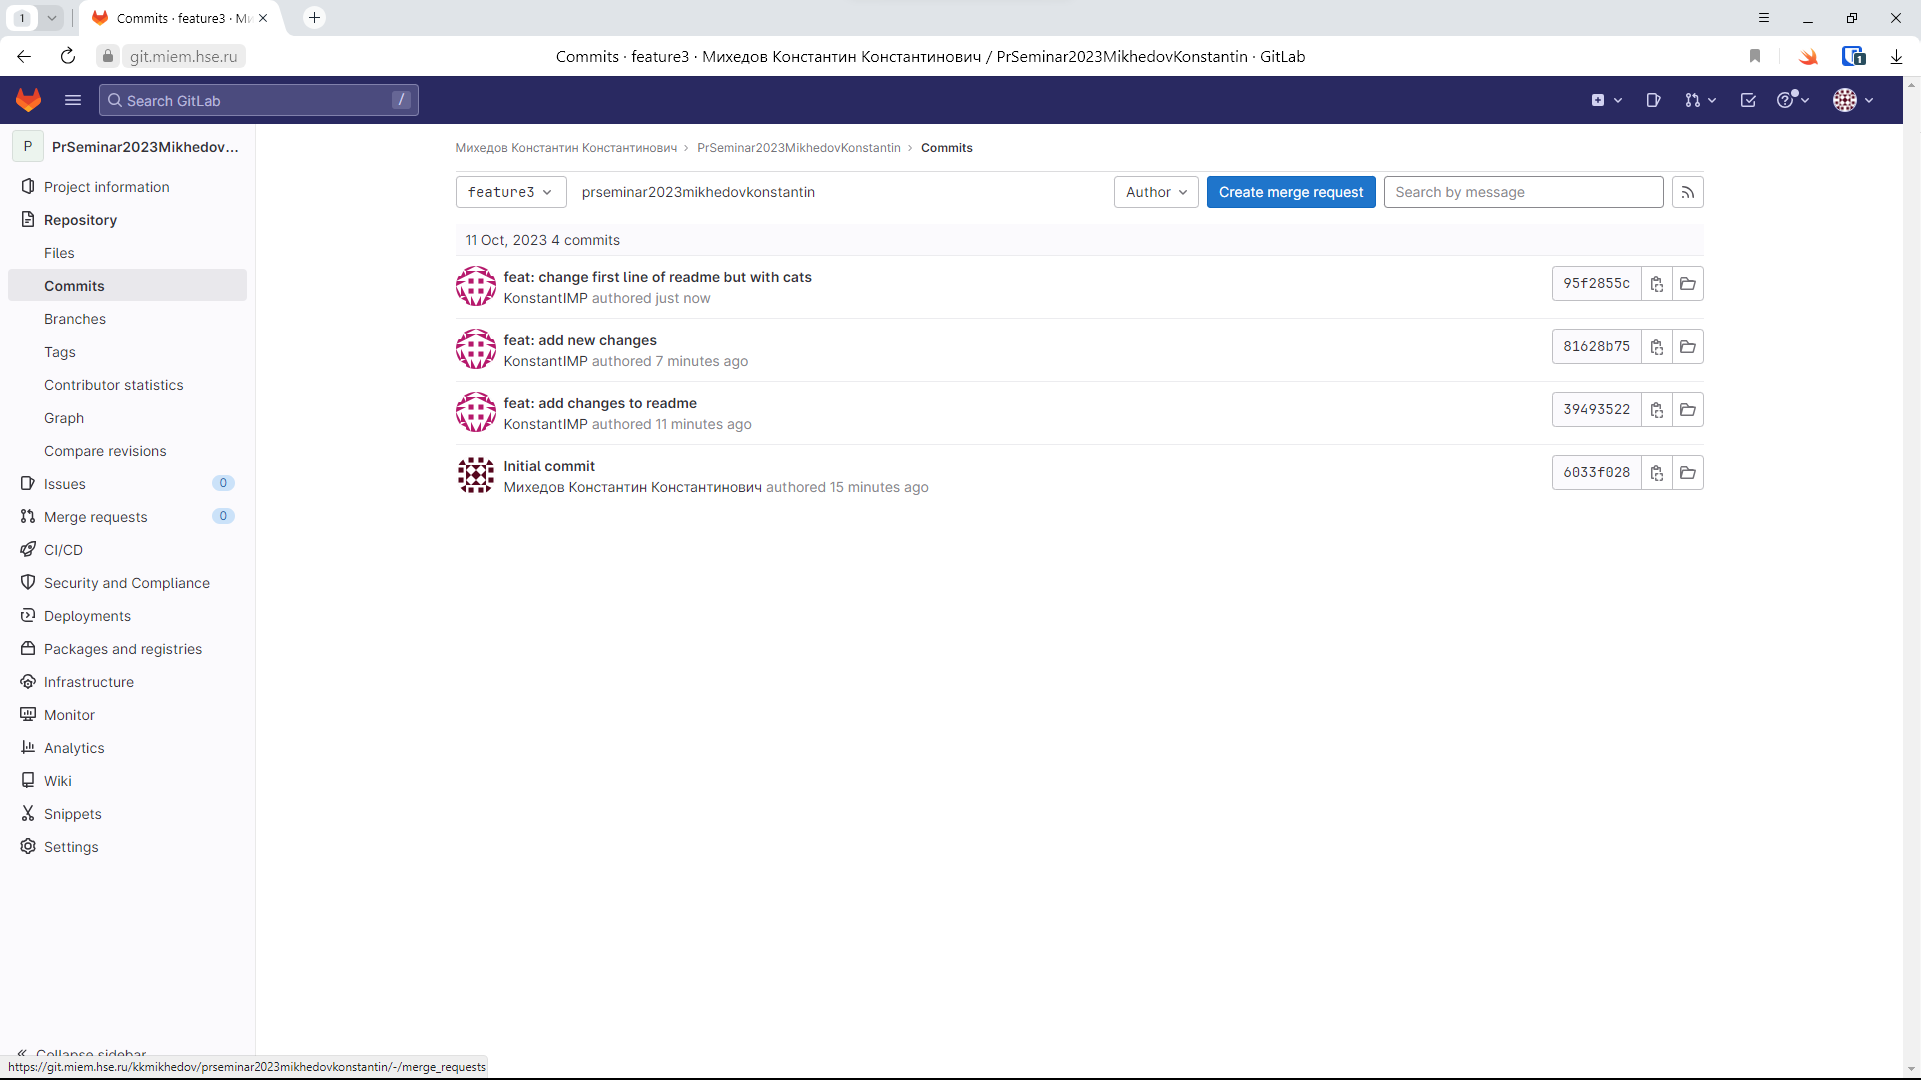
\includegraphics[width=\textwidth]{1_ (24)}
    \caption{Переходим на вкладку <<Merge requests>>}
  \end{figure}

  \begin{figure}[H]
    \centering
    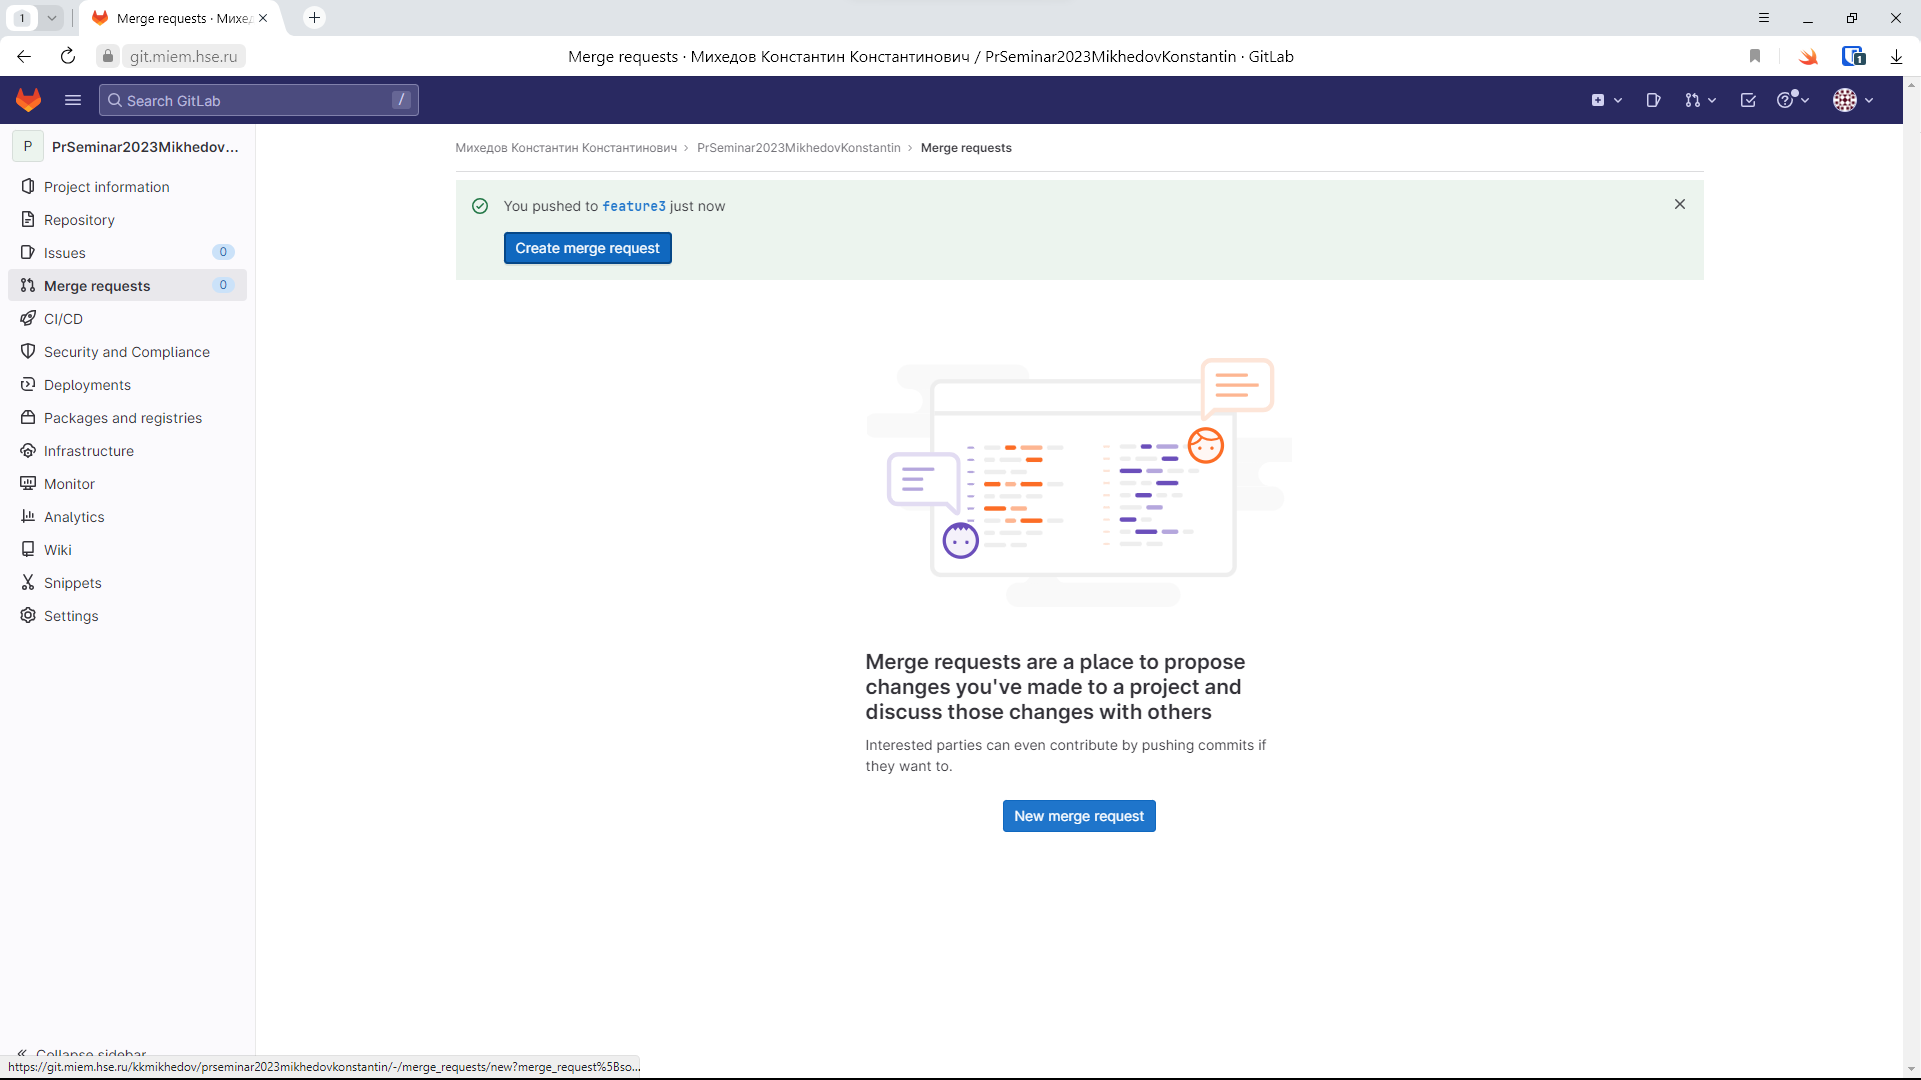
\includegraphics[width=\textwidth]{1_ (23)}
    \caption{Нажимаем на кнопку <<Create merge request>>}
  \end{figure}

  \begin{figure}[H]
    \centering
    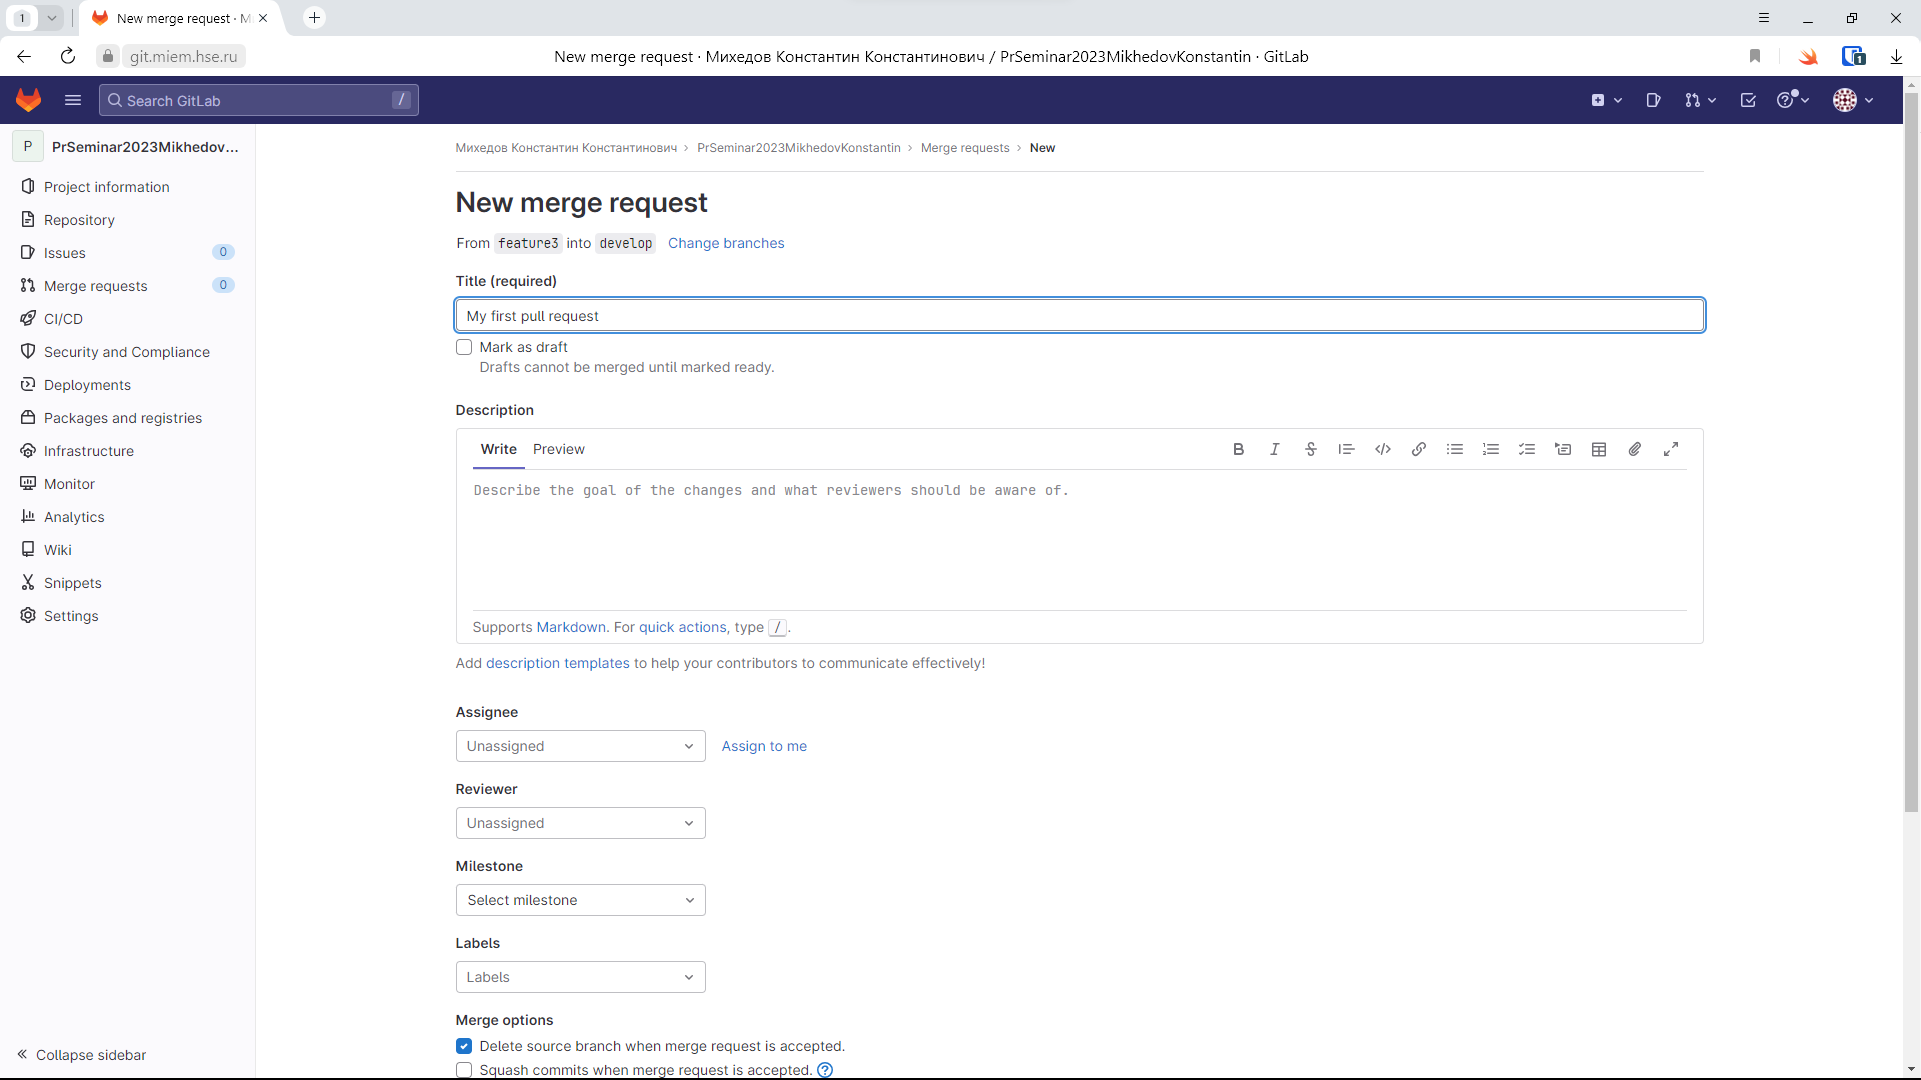
\includegraphics[width=\textwidth]{1_ (22)}
    \caption{Источник - feature3, цель - develop}
  \end{figure}

  \begin{figure}[H]
    \centering
    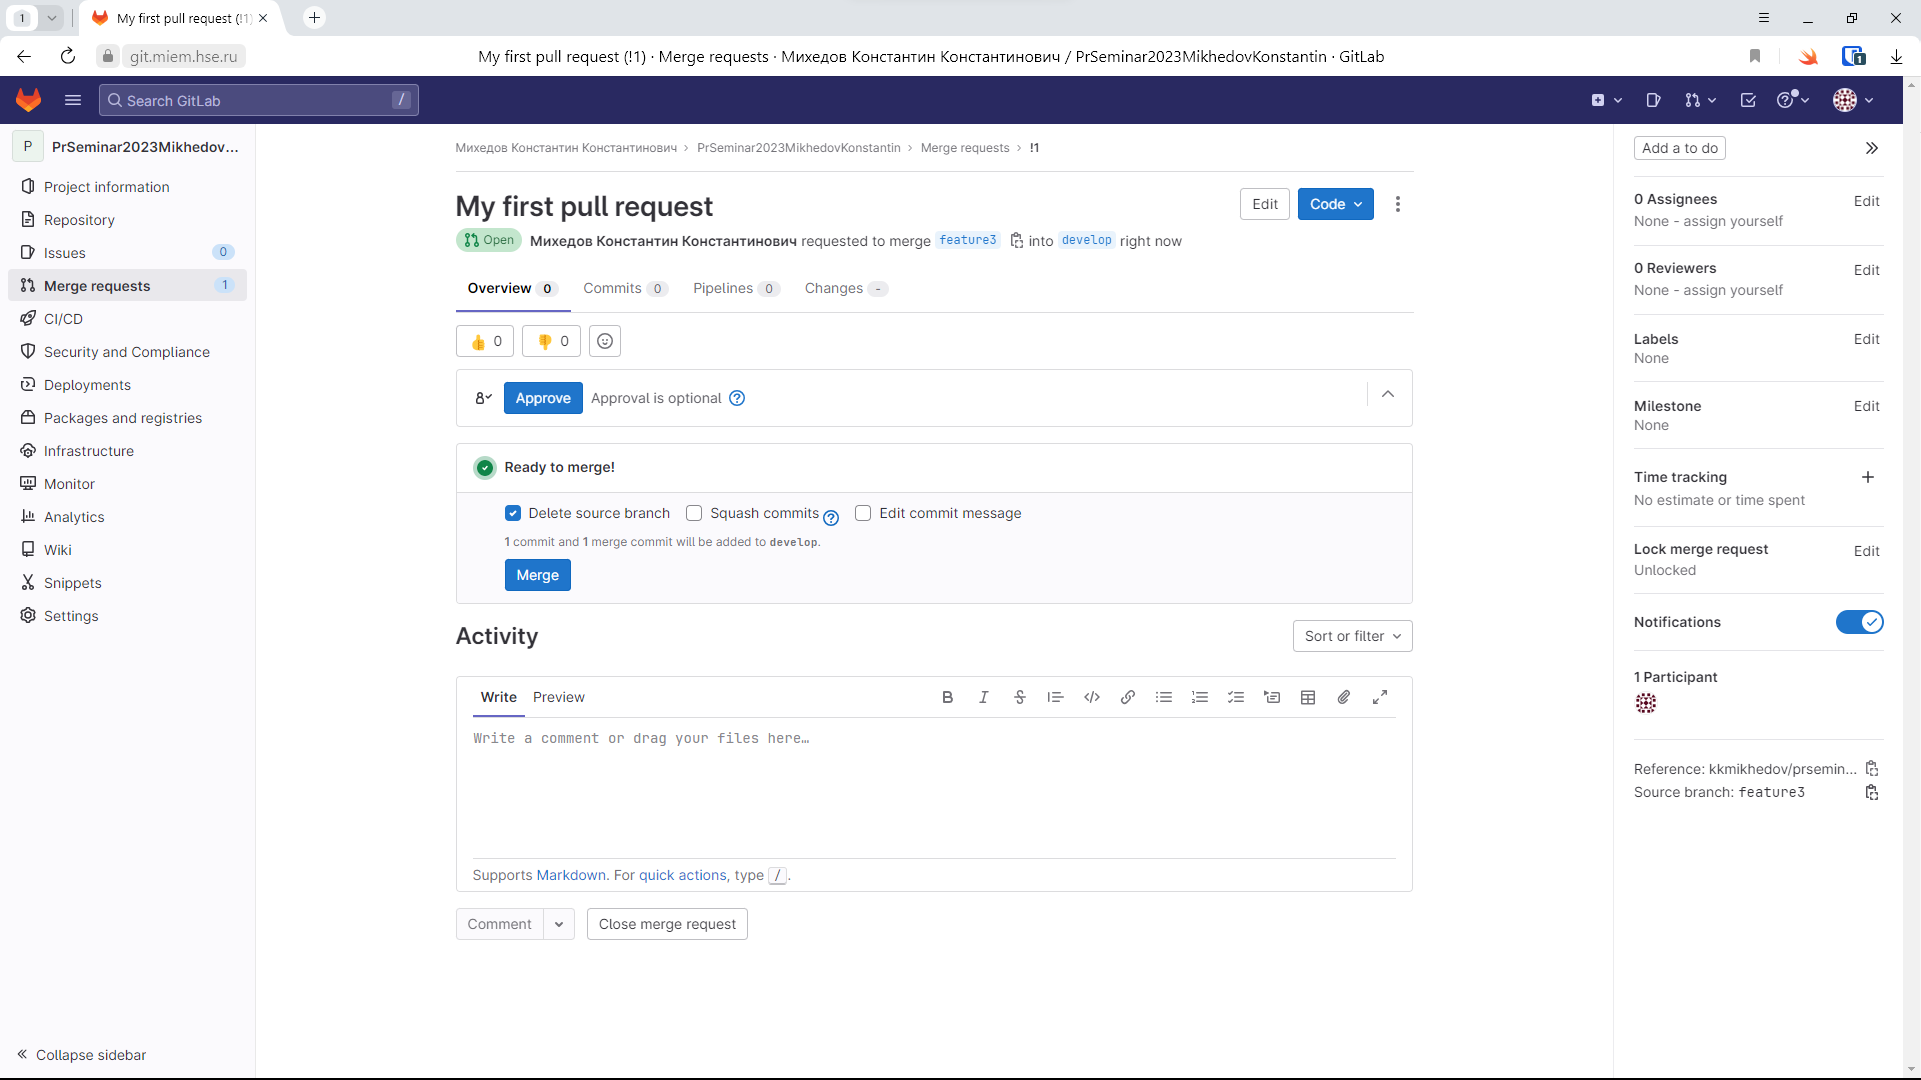
\includegraphics[width=\textwidth]{1_ (21)}
    \caption{Merge request создан}
  \end{figure}

  \begin{figure}[H]
    \centering
    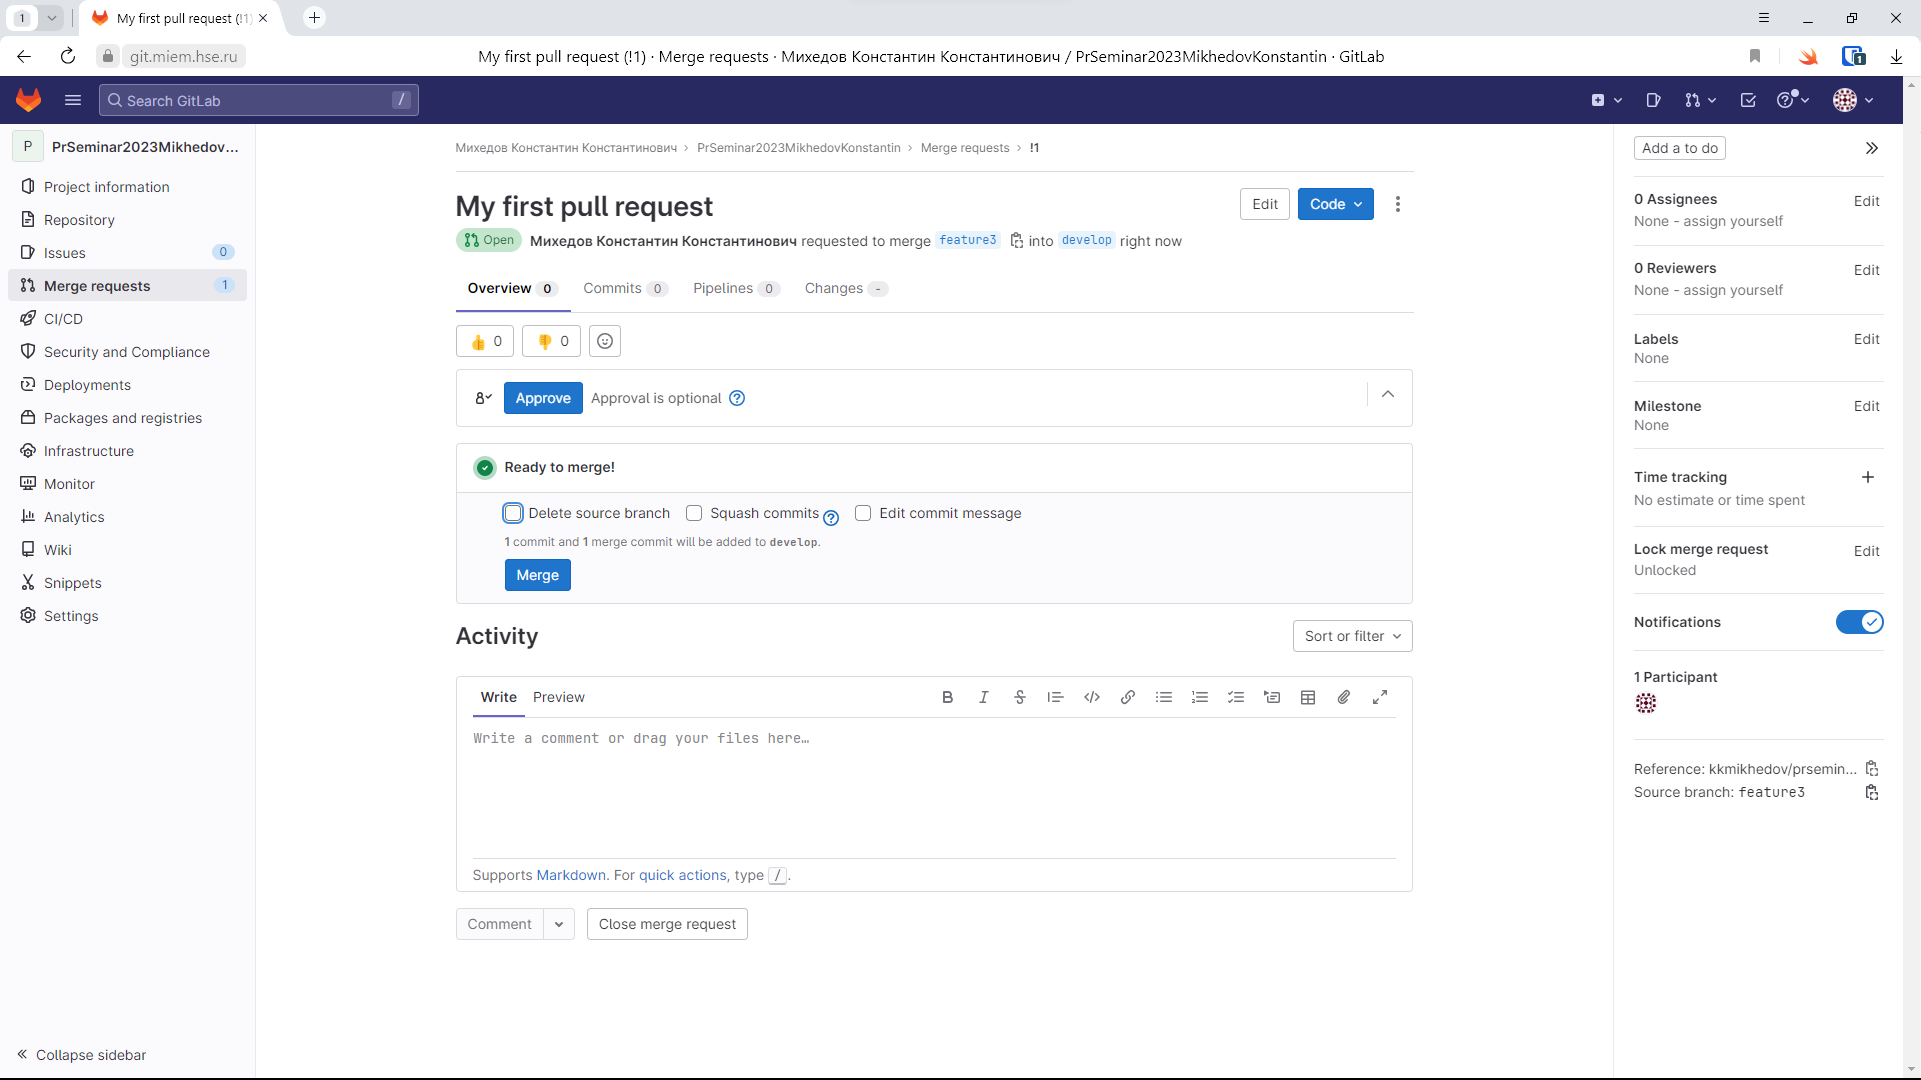
\includegraphics[width=\textwidth]{1_ (20)}
    \caption{Отключаем удаление ветки после закрытия merge request и нажимаем кнопку <<merge>>}
  \end{figure}

  \begin{figure}[H]
    \centering
    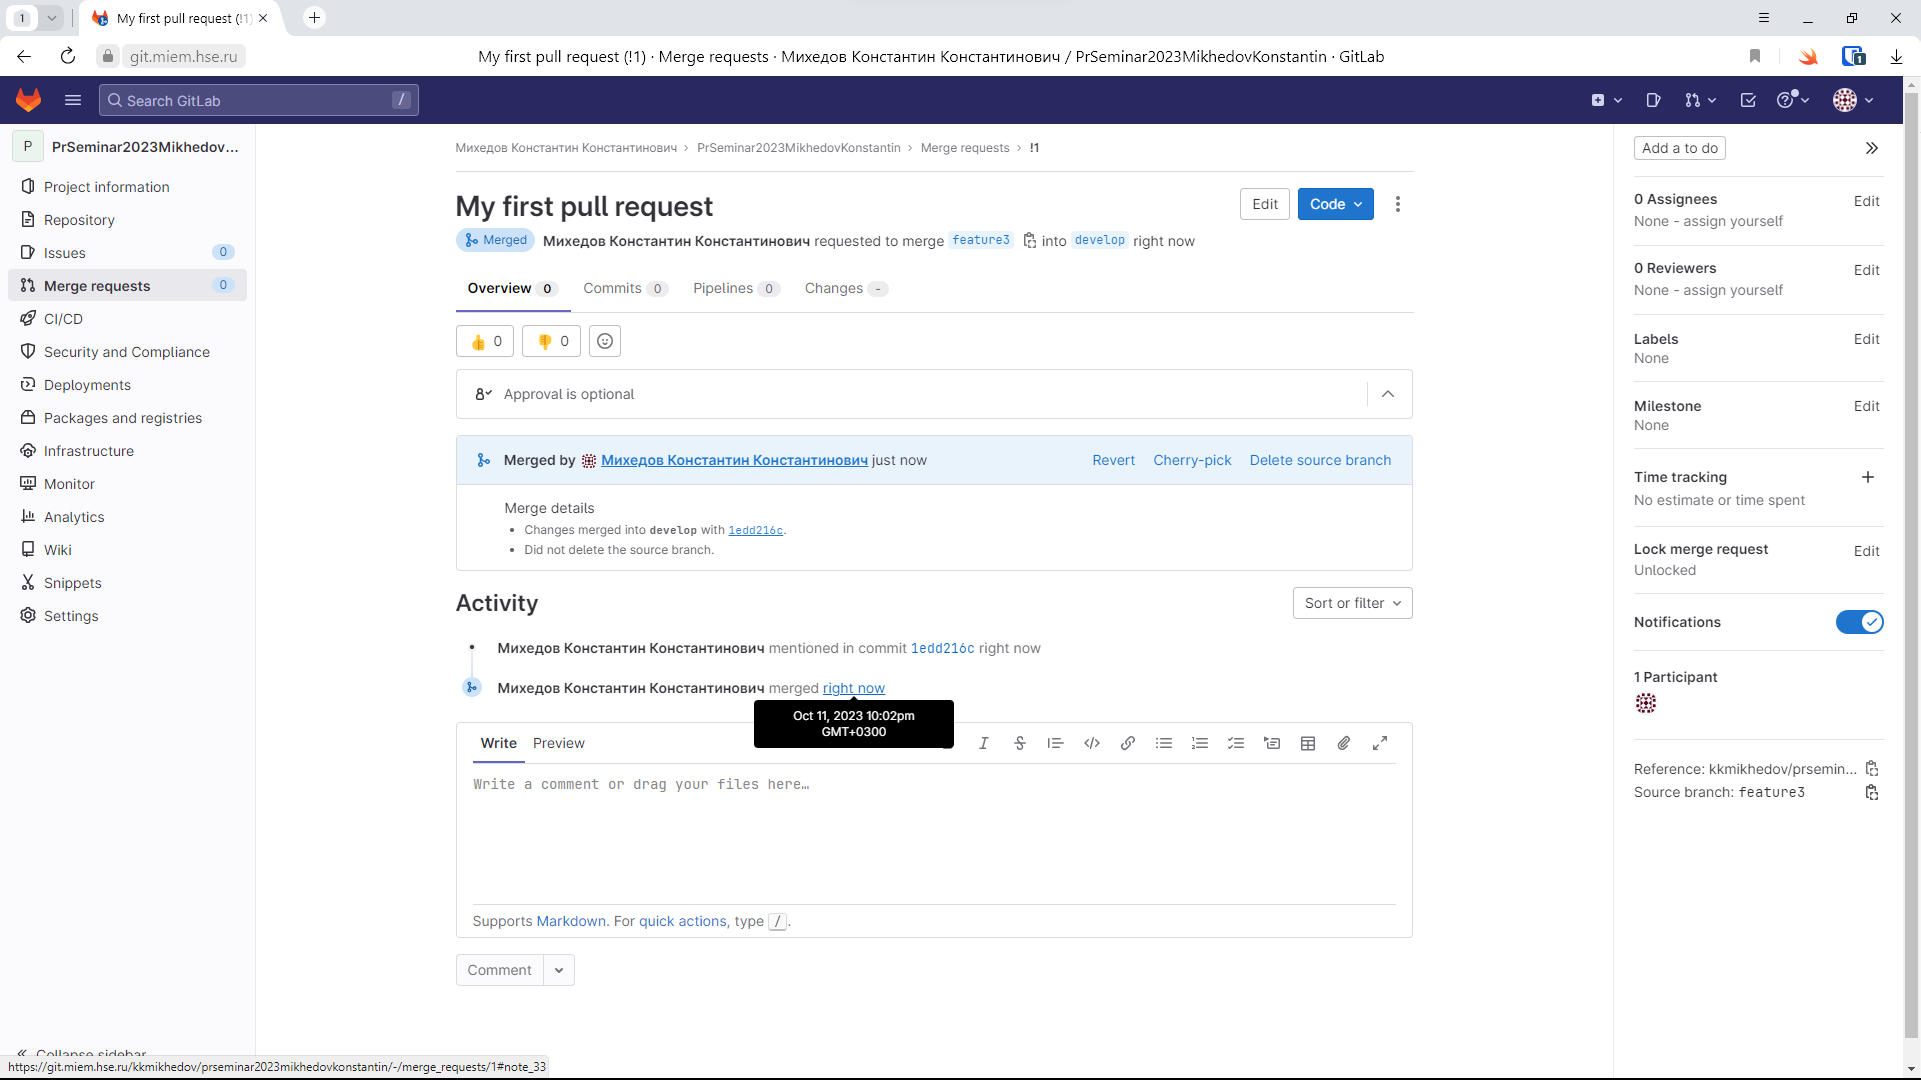
\includegraphics[width=\textwidth]{1_ (19)}
    \caption{Merge request успешно выполнен}
  \end{figure}

  \textbf{Ссылка на merge request (feature3 -> develop):} \href{https://git.miem.hse.ru/kkmikhedov/prseminar2023mikhedovkonstantin/-/merge_requests/1}{где-то здесь}

  Теперь попробуем замерджить ветку feature2 с изменениями того же файла в том же месте в develop:

  \begin{figure}[H]
    \centering
    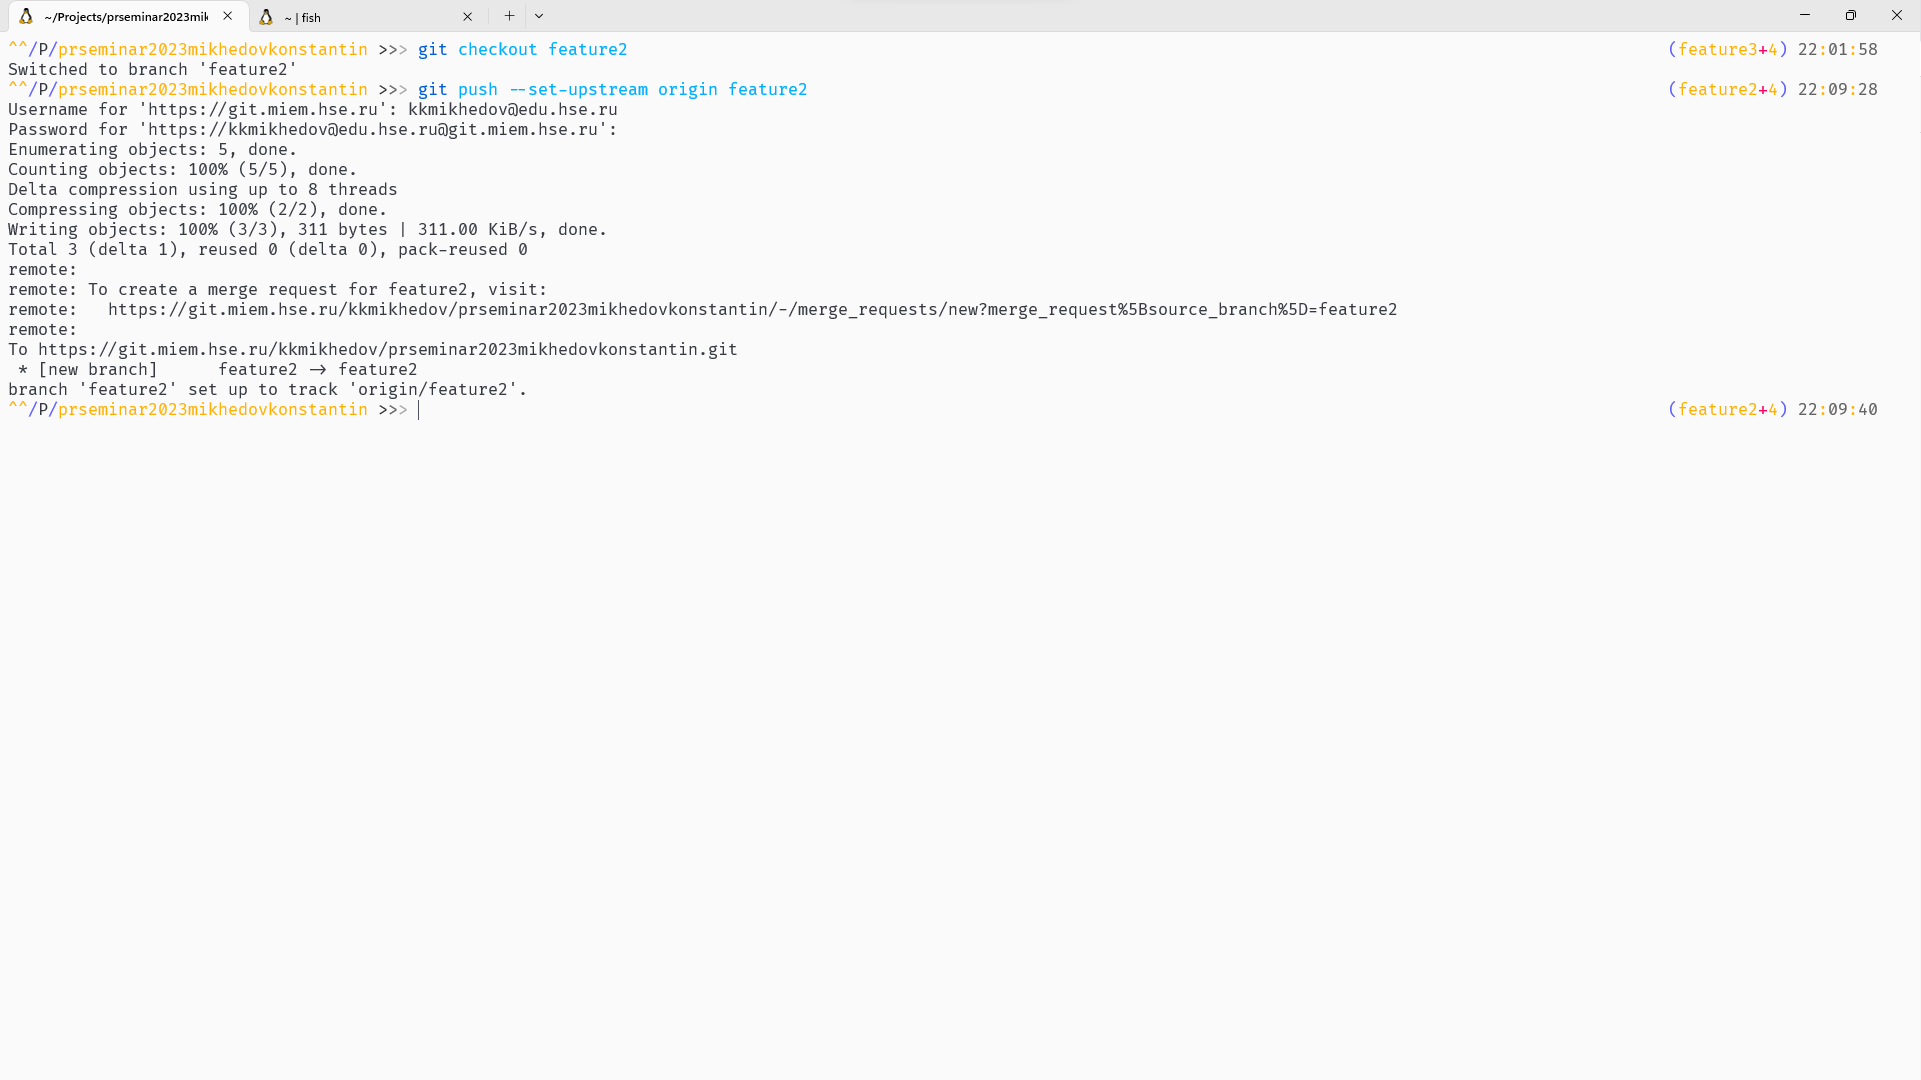
\includegraphics[width=\textwidth]{1_ (17)}
    \caption{Отправляем ветку на удаленный репозиторий}
  \end{figure}

  \begin{figure}[H]
    \centering
    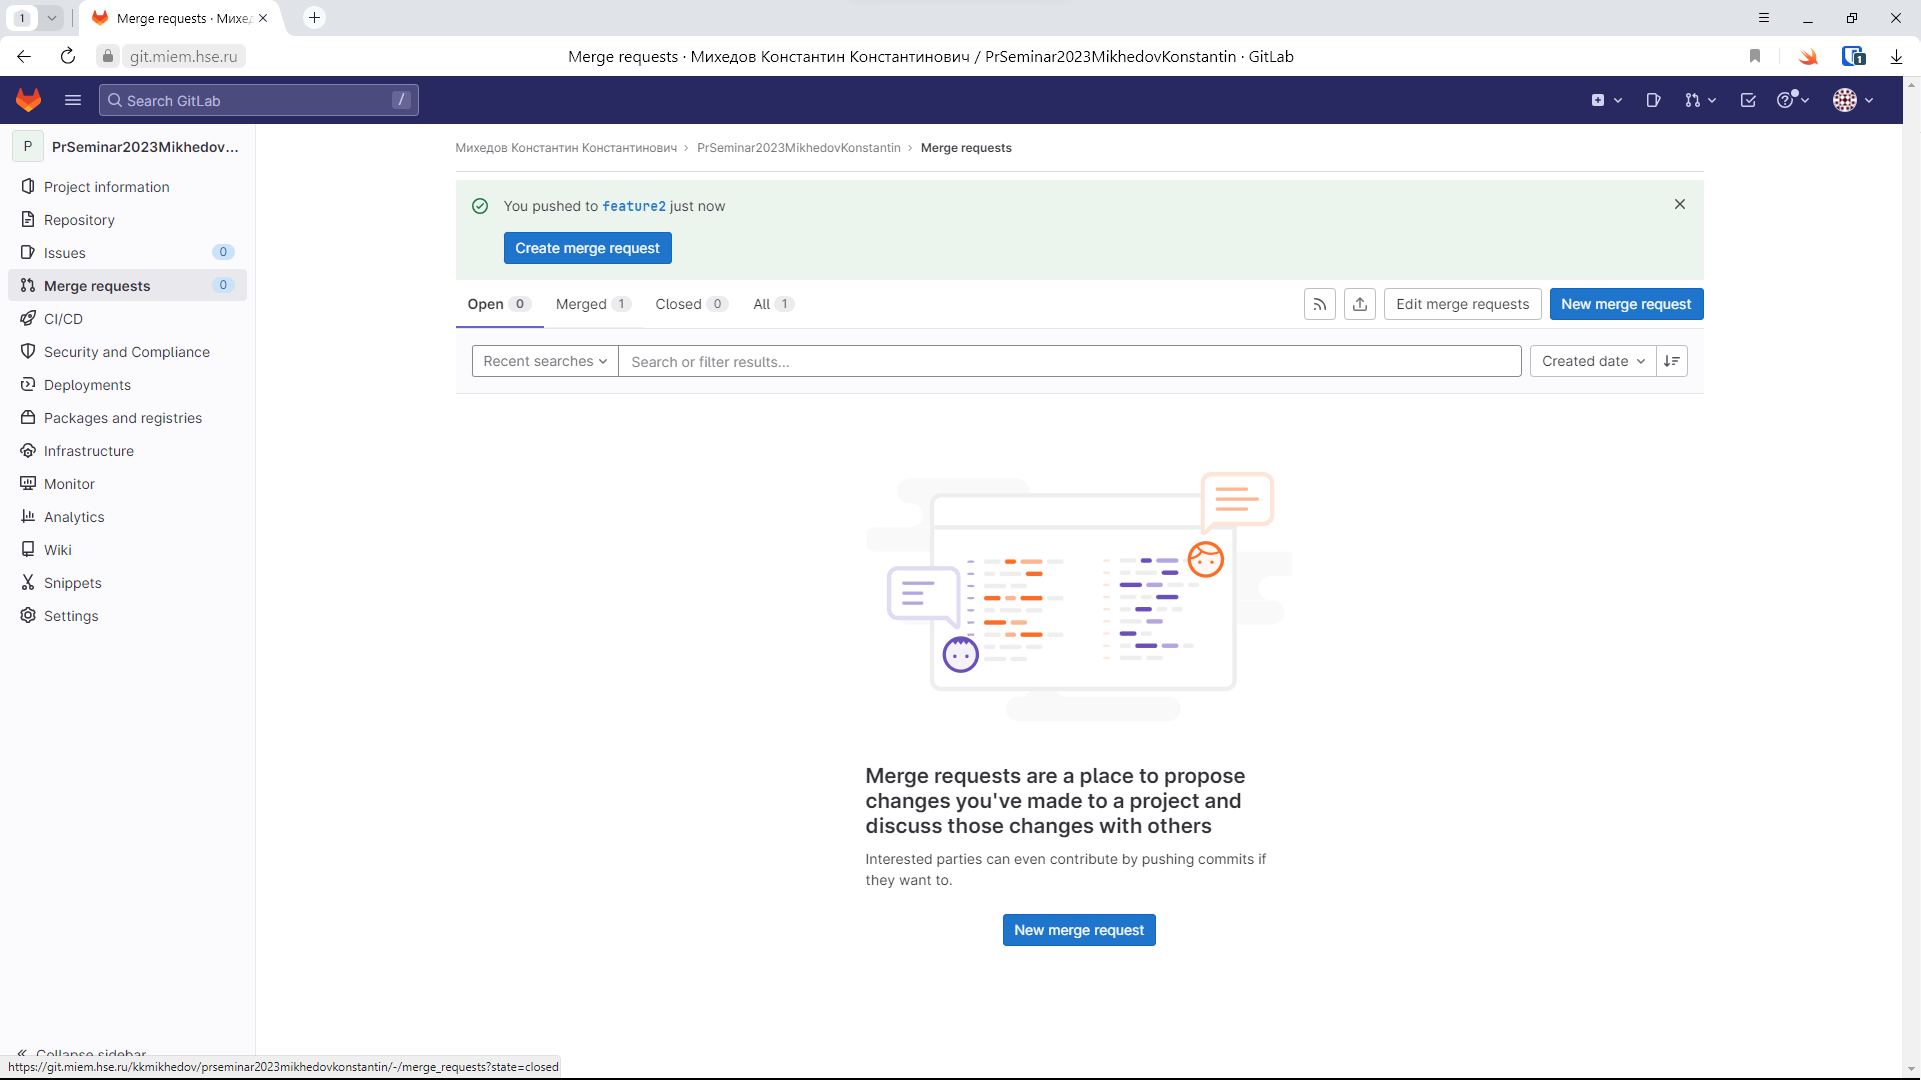
\includegraphics[width=\textwidth]{1_ (16)}
    \caption{Нажимаем <<Create merge request>>}
  \end{figure}

  \begin{figure}[H]
    \centering
    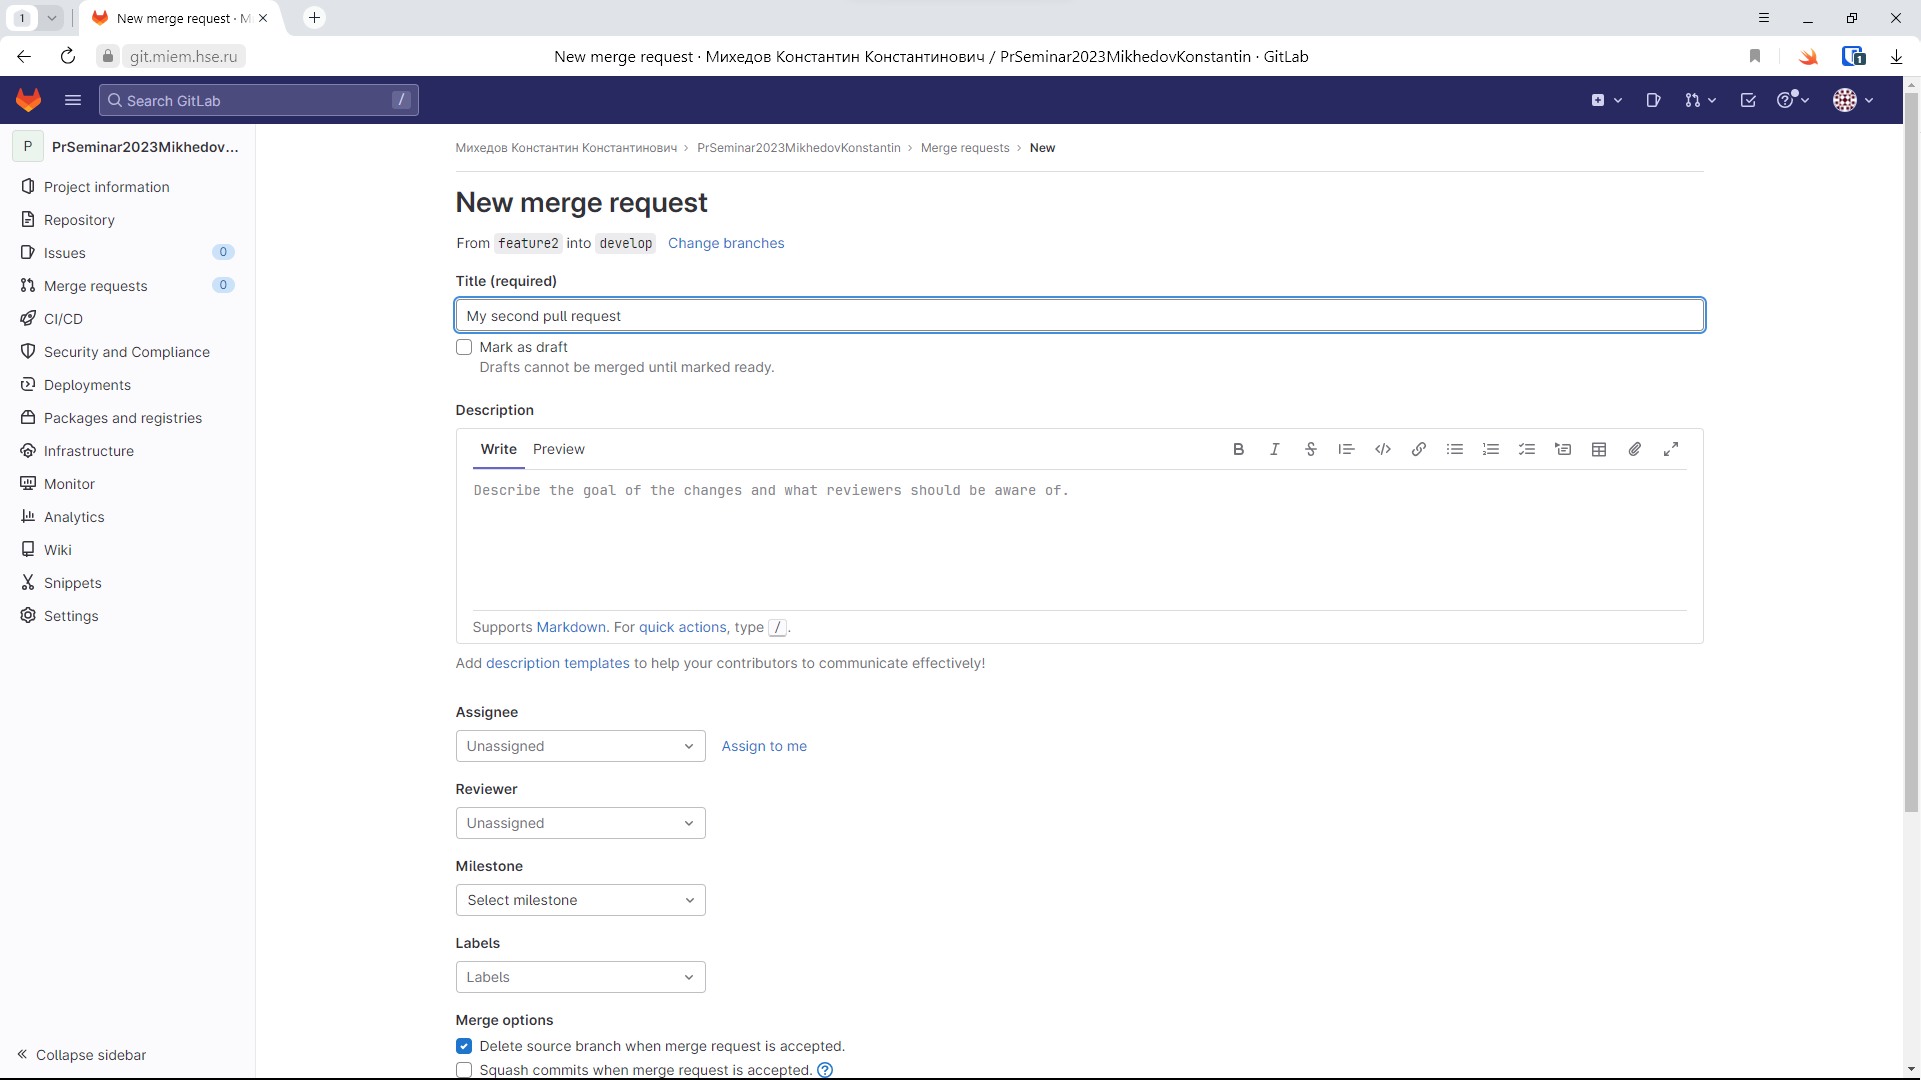
\includegraphics[width=\textwidth]{1_ (15)}
    \caption{Указываем информацию о merge request}
  \end{figure}

  \begin{figure}[H]
    \centering
    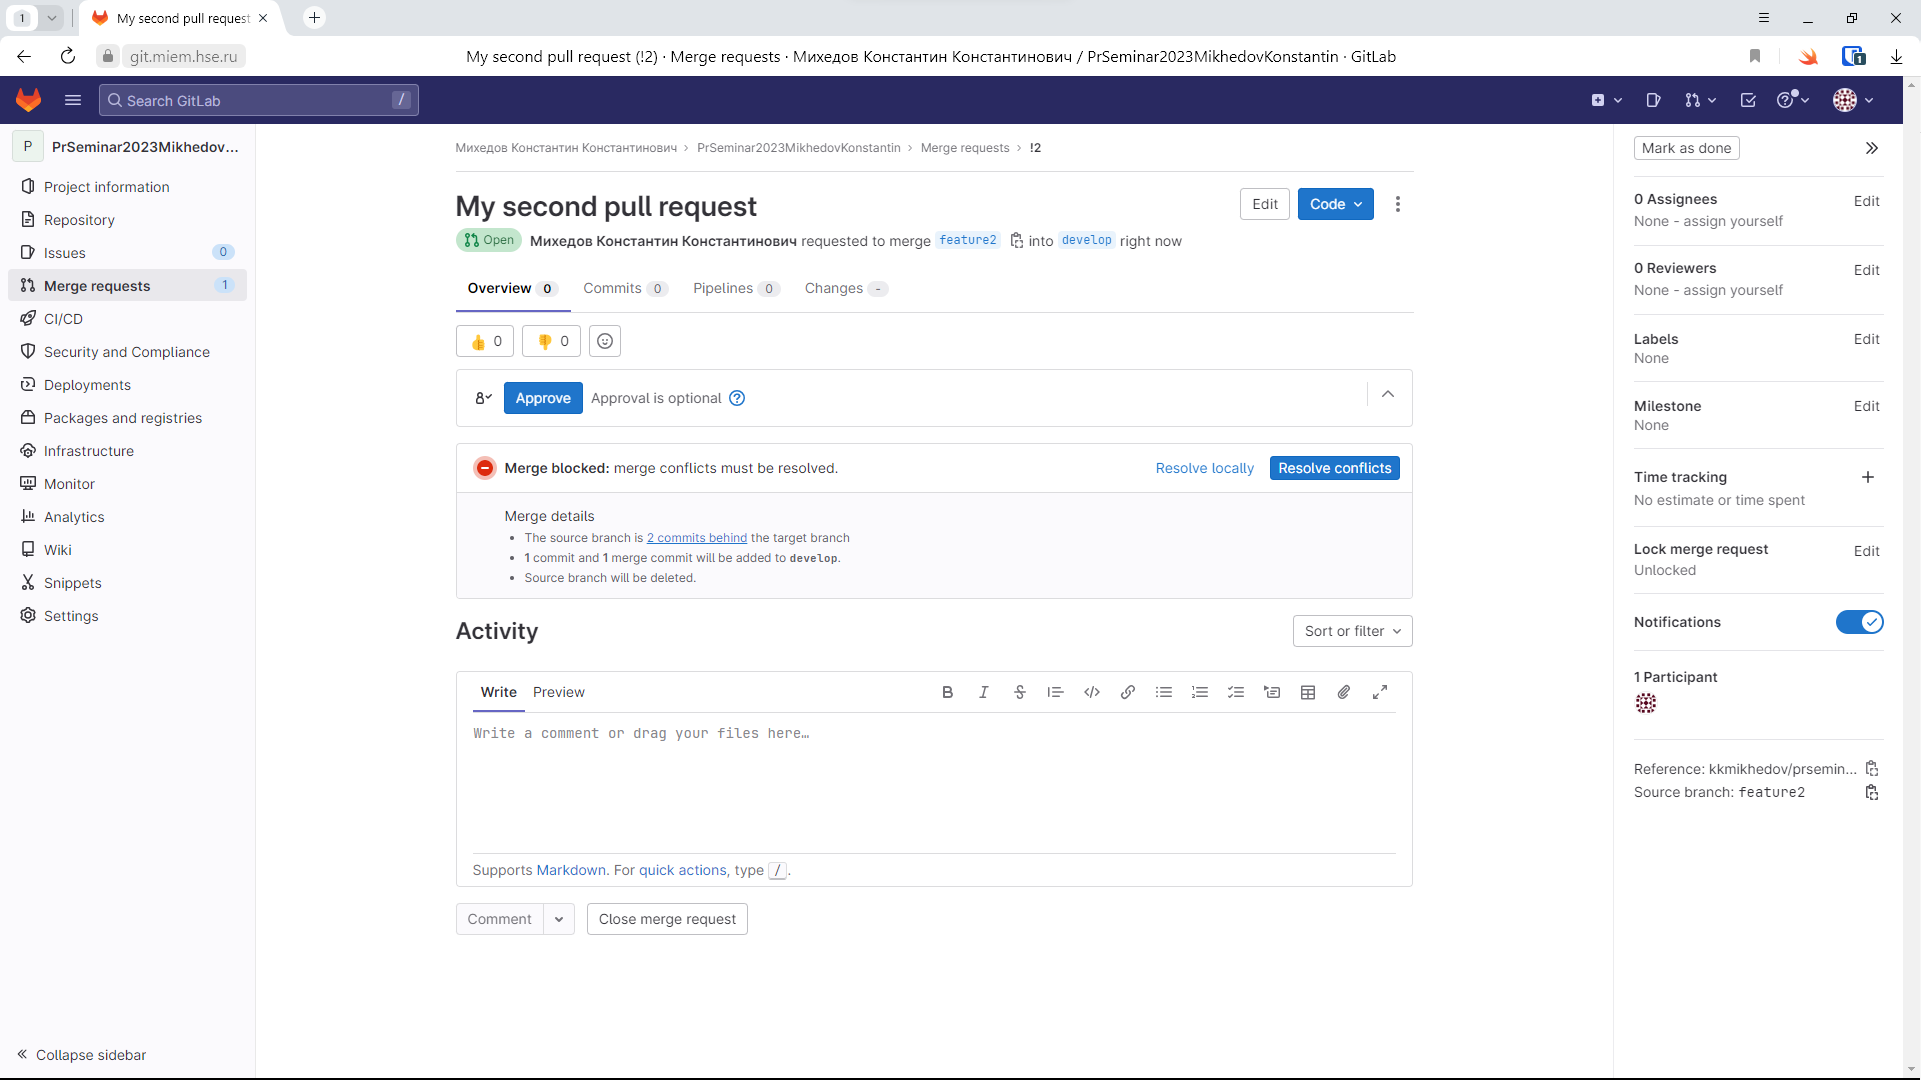
\includegraphics[width=\textwidth]{1_ (14)}
    \caption{Видим сообщение о наличии конфликтов}
  \end{figure}

  Необходимо разрешить полученный конфликт локально:

  \begin{figure}[H]
    \centering
    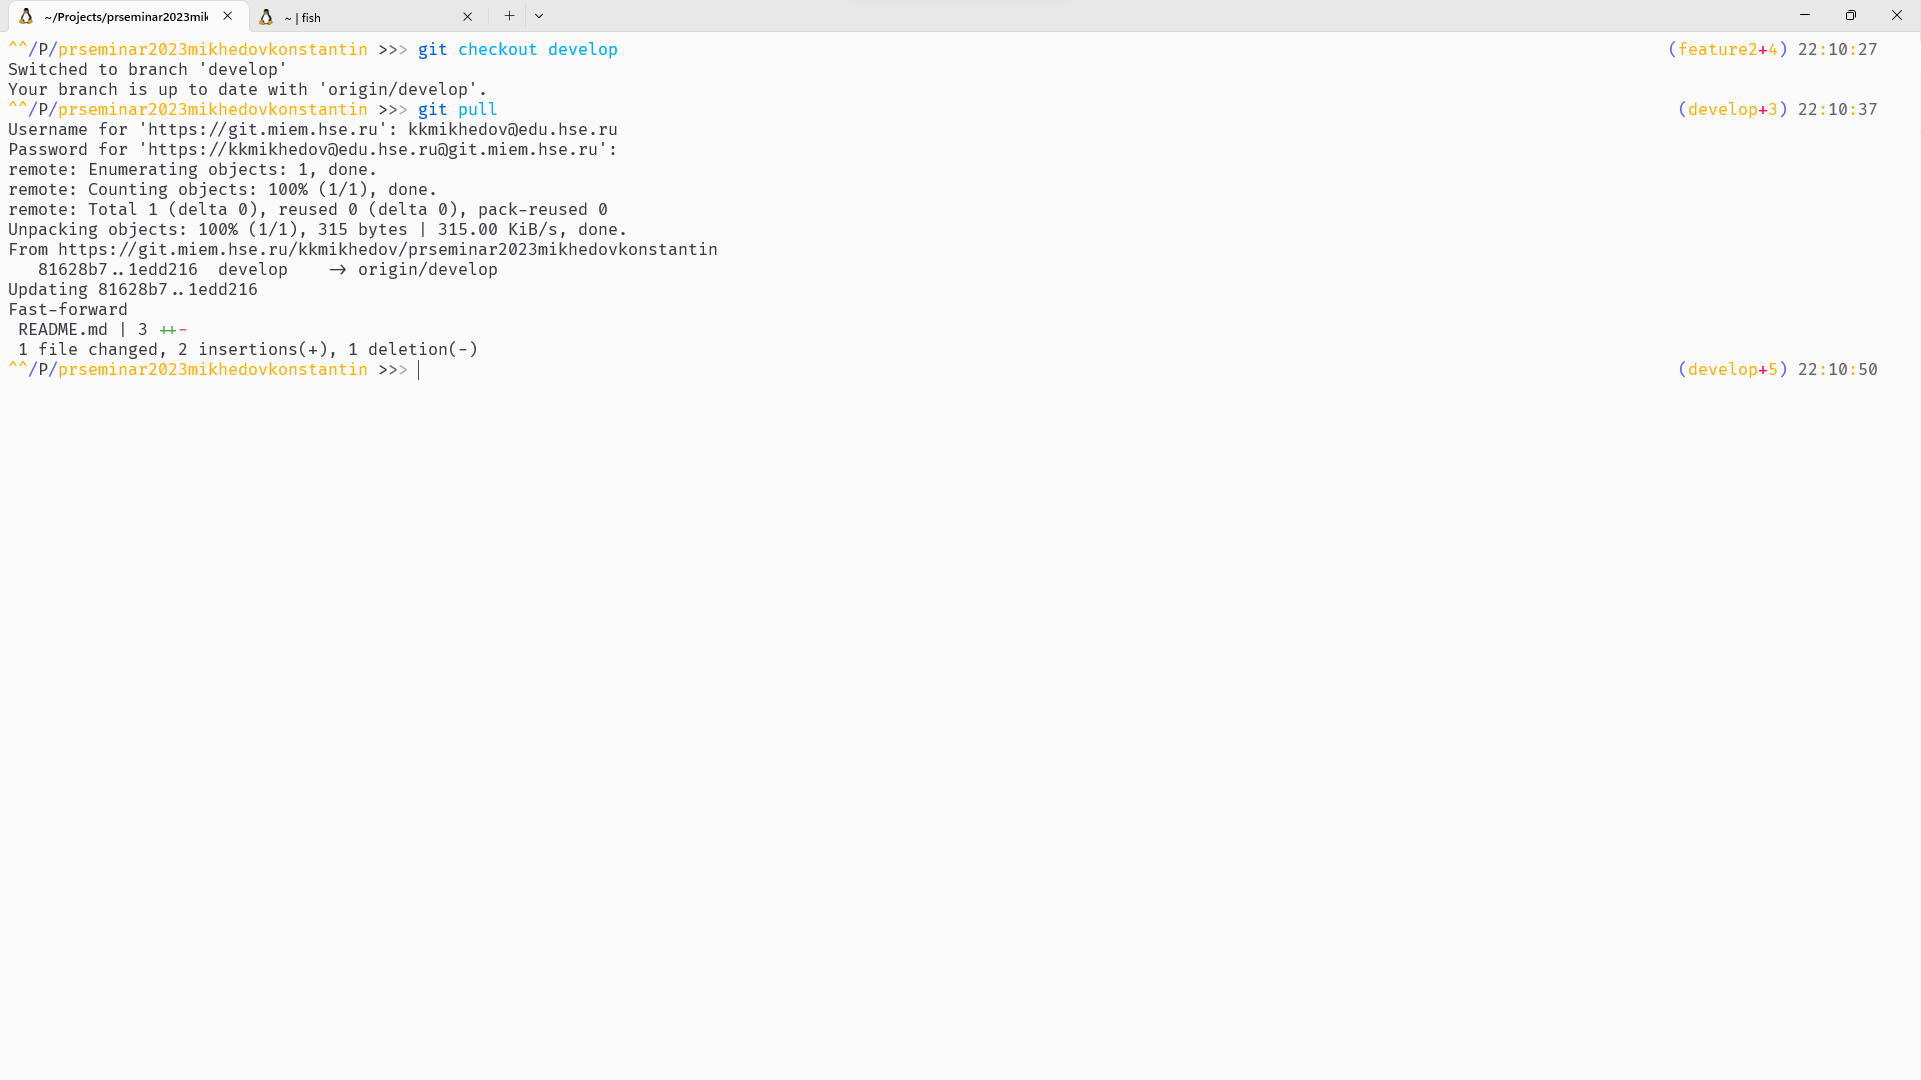
\includegraphics[width=\textwidth]{1_ (13)}
    \caption{Синхронизируем локальную копию с удаленным репозиторием}
  \end{figure}

  \begin{figure}[H]
    \centering
    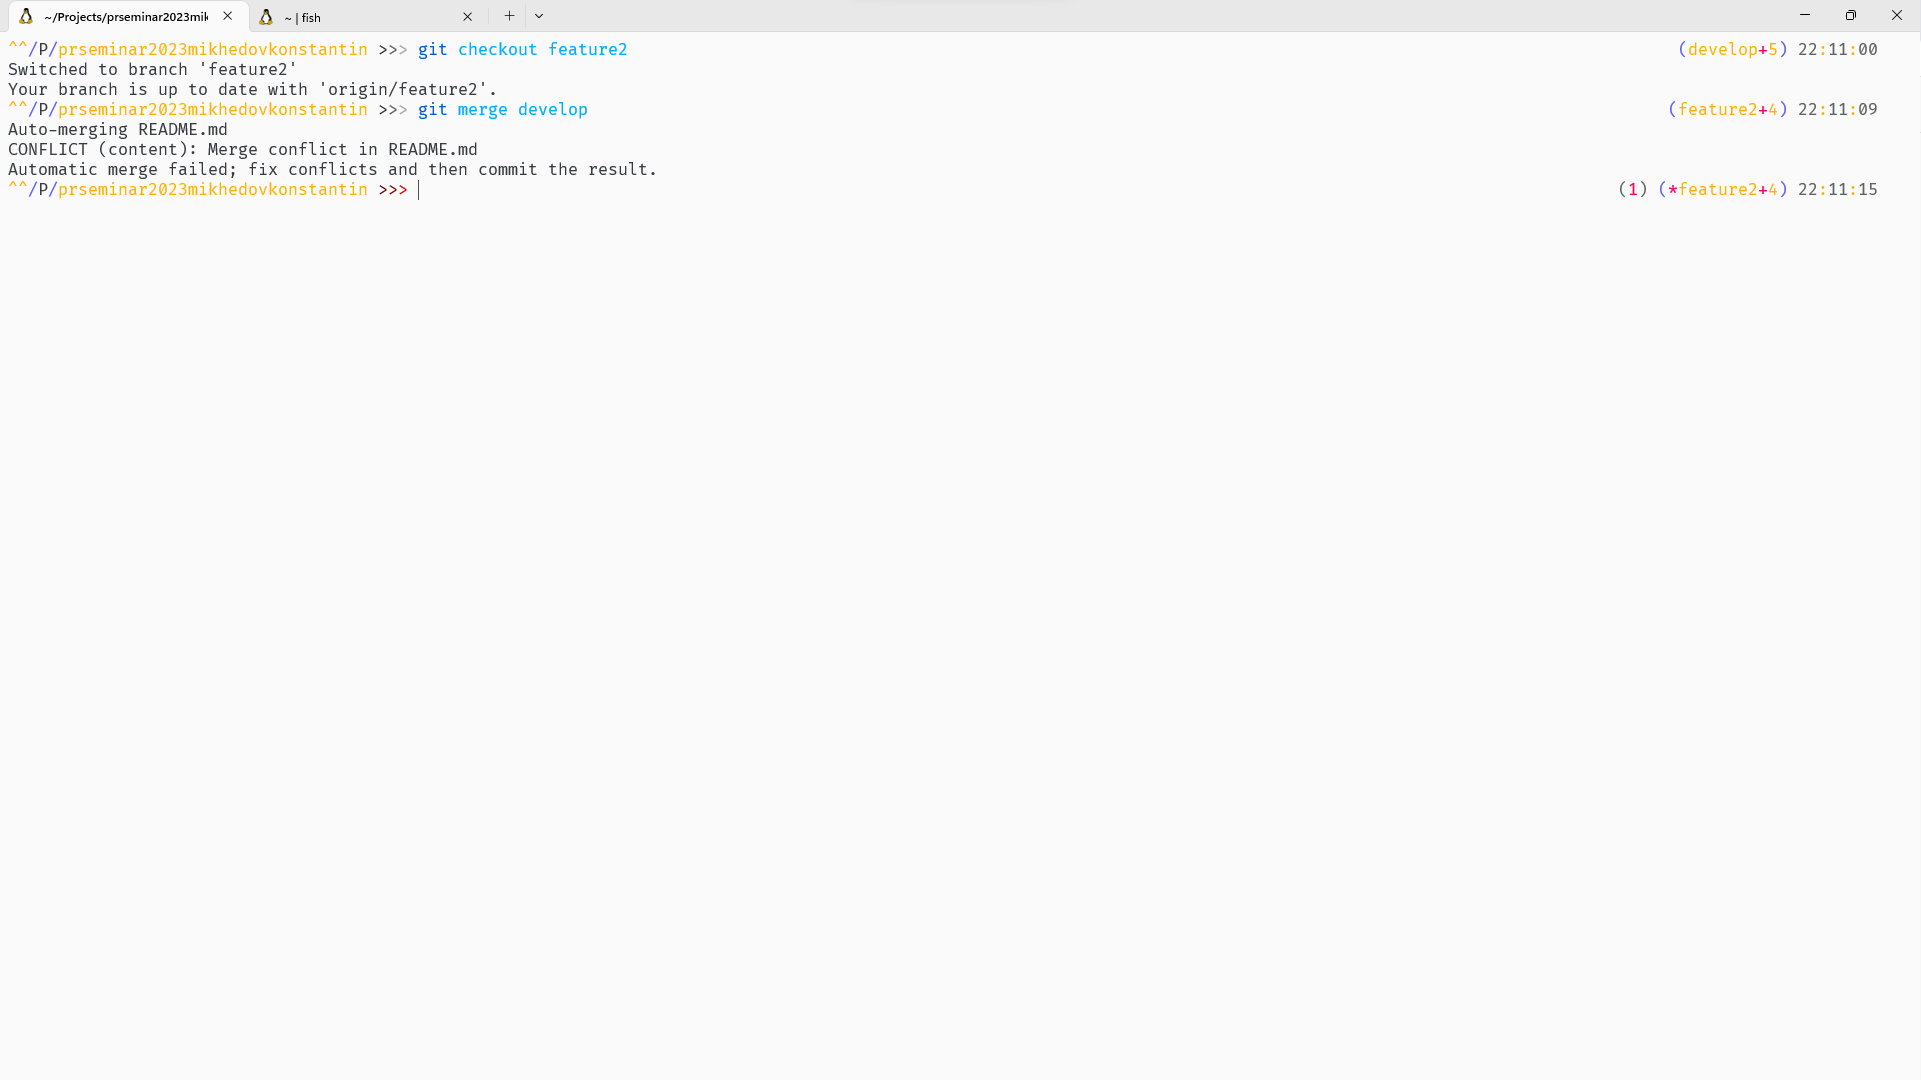
\includegraphics[width=\textwidth]{1_ (12)}
    \caption{Пробуем вмерджить ветку develop в ветку feature2}
  \end{figure}

  Получено сообщение о наличии конфликта в файле README.md, посмотрим его содержимое:

  \begin{figure}[H]
    \centering
    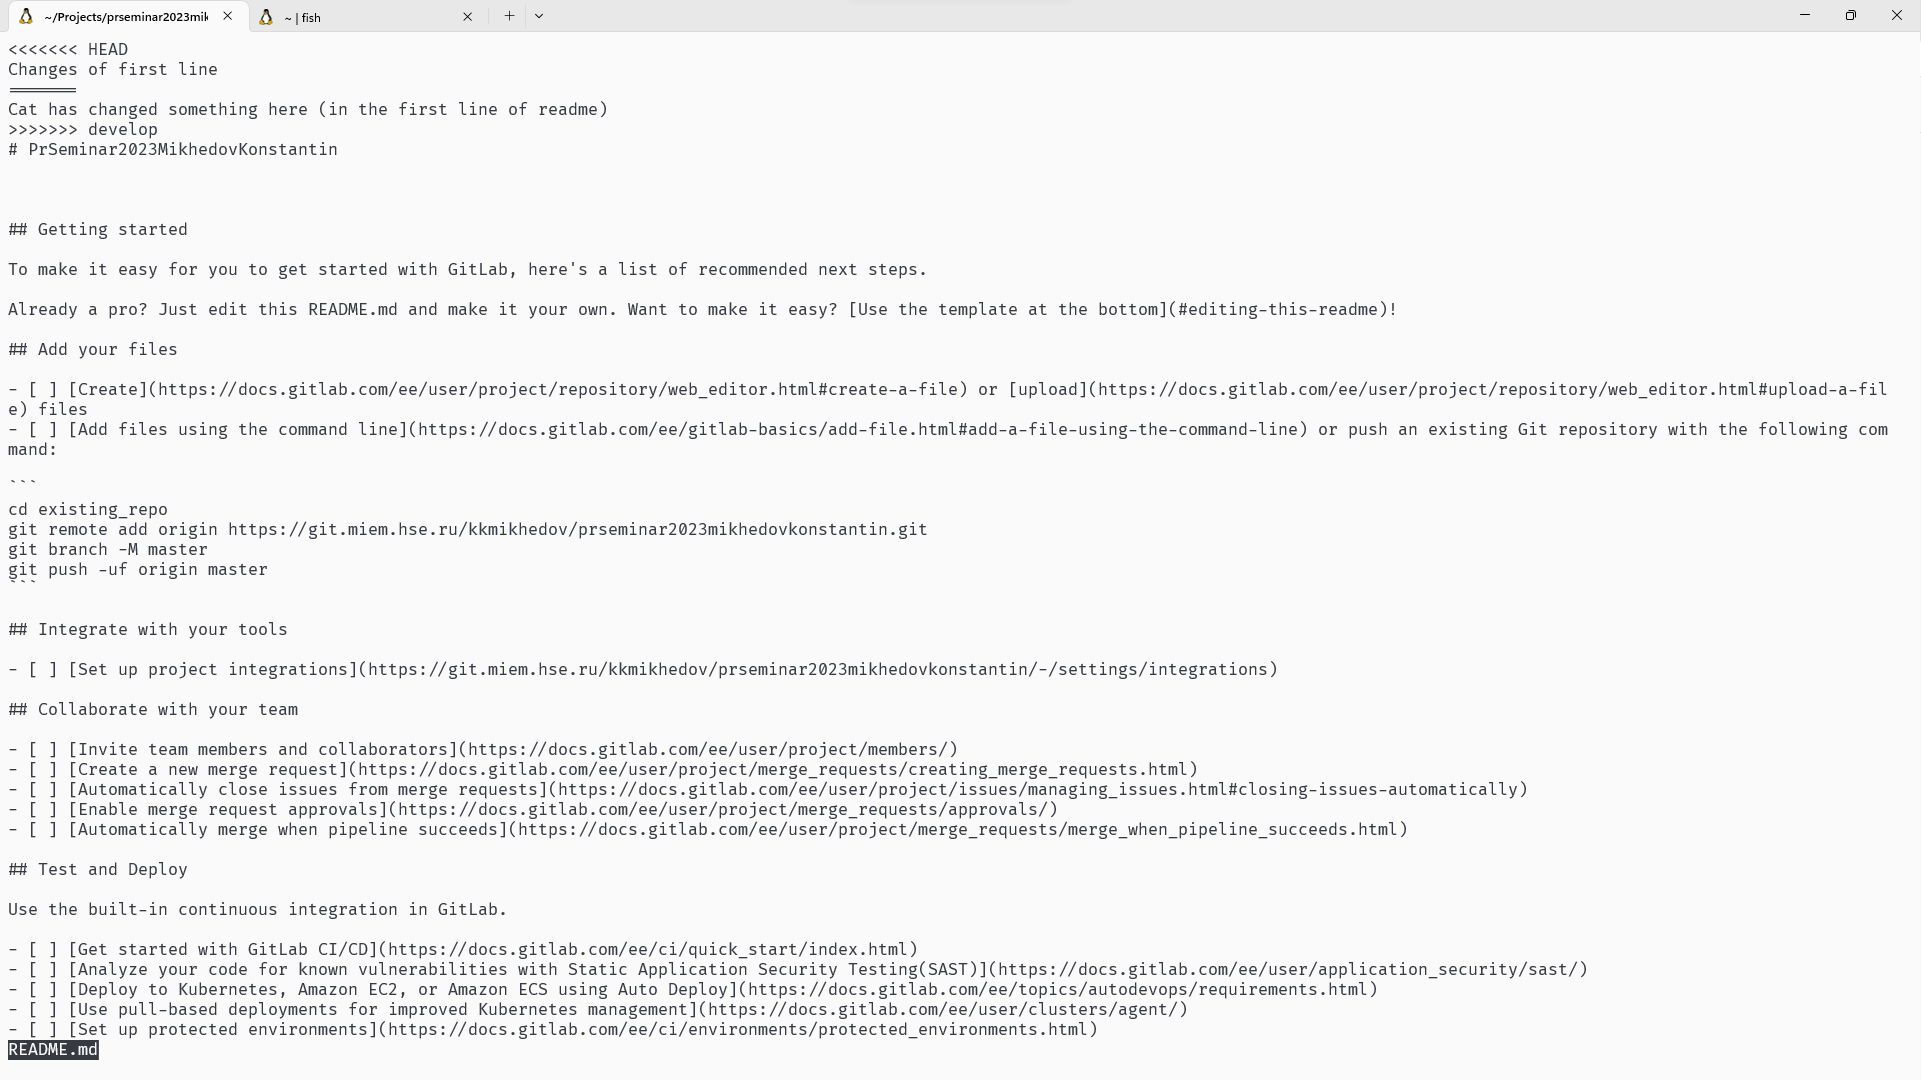
\includegraphics[width=\textwidth]{1_ (11)}
    \caption{Видим конфликт в первых двух строчках}
  \end{figure}

  \begin{figure}[H]
    \centering
    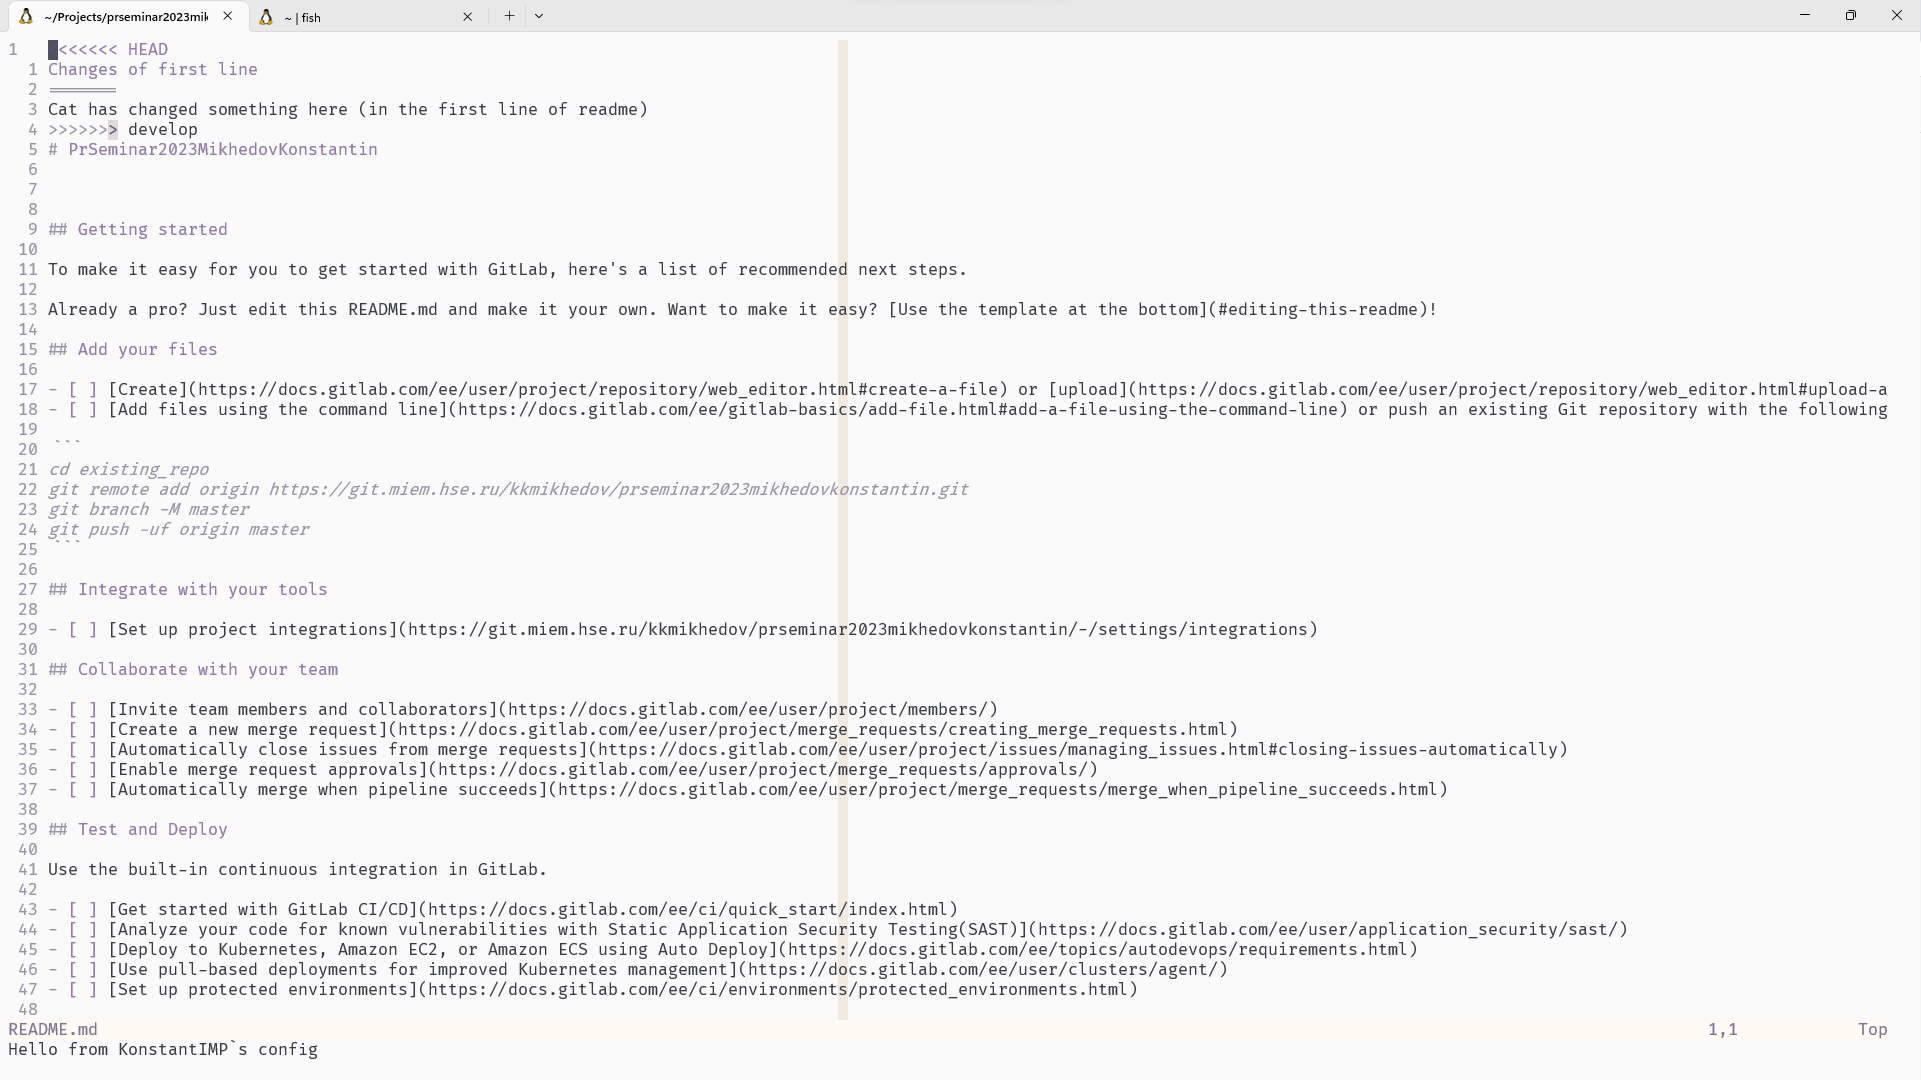
\includegraphics[width=\textwidth]{1_ (10)}
    \caption{Открываем README.md через vim и правим конфликт}
  \end{figure}

  \begin{figure}[H]
    \centering
    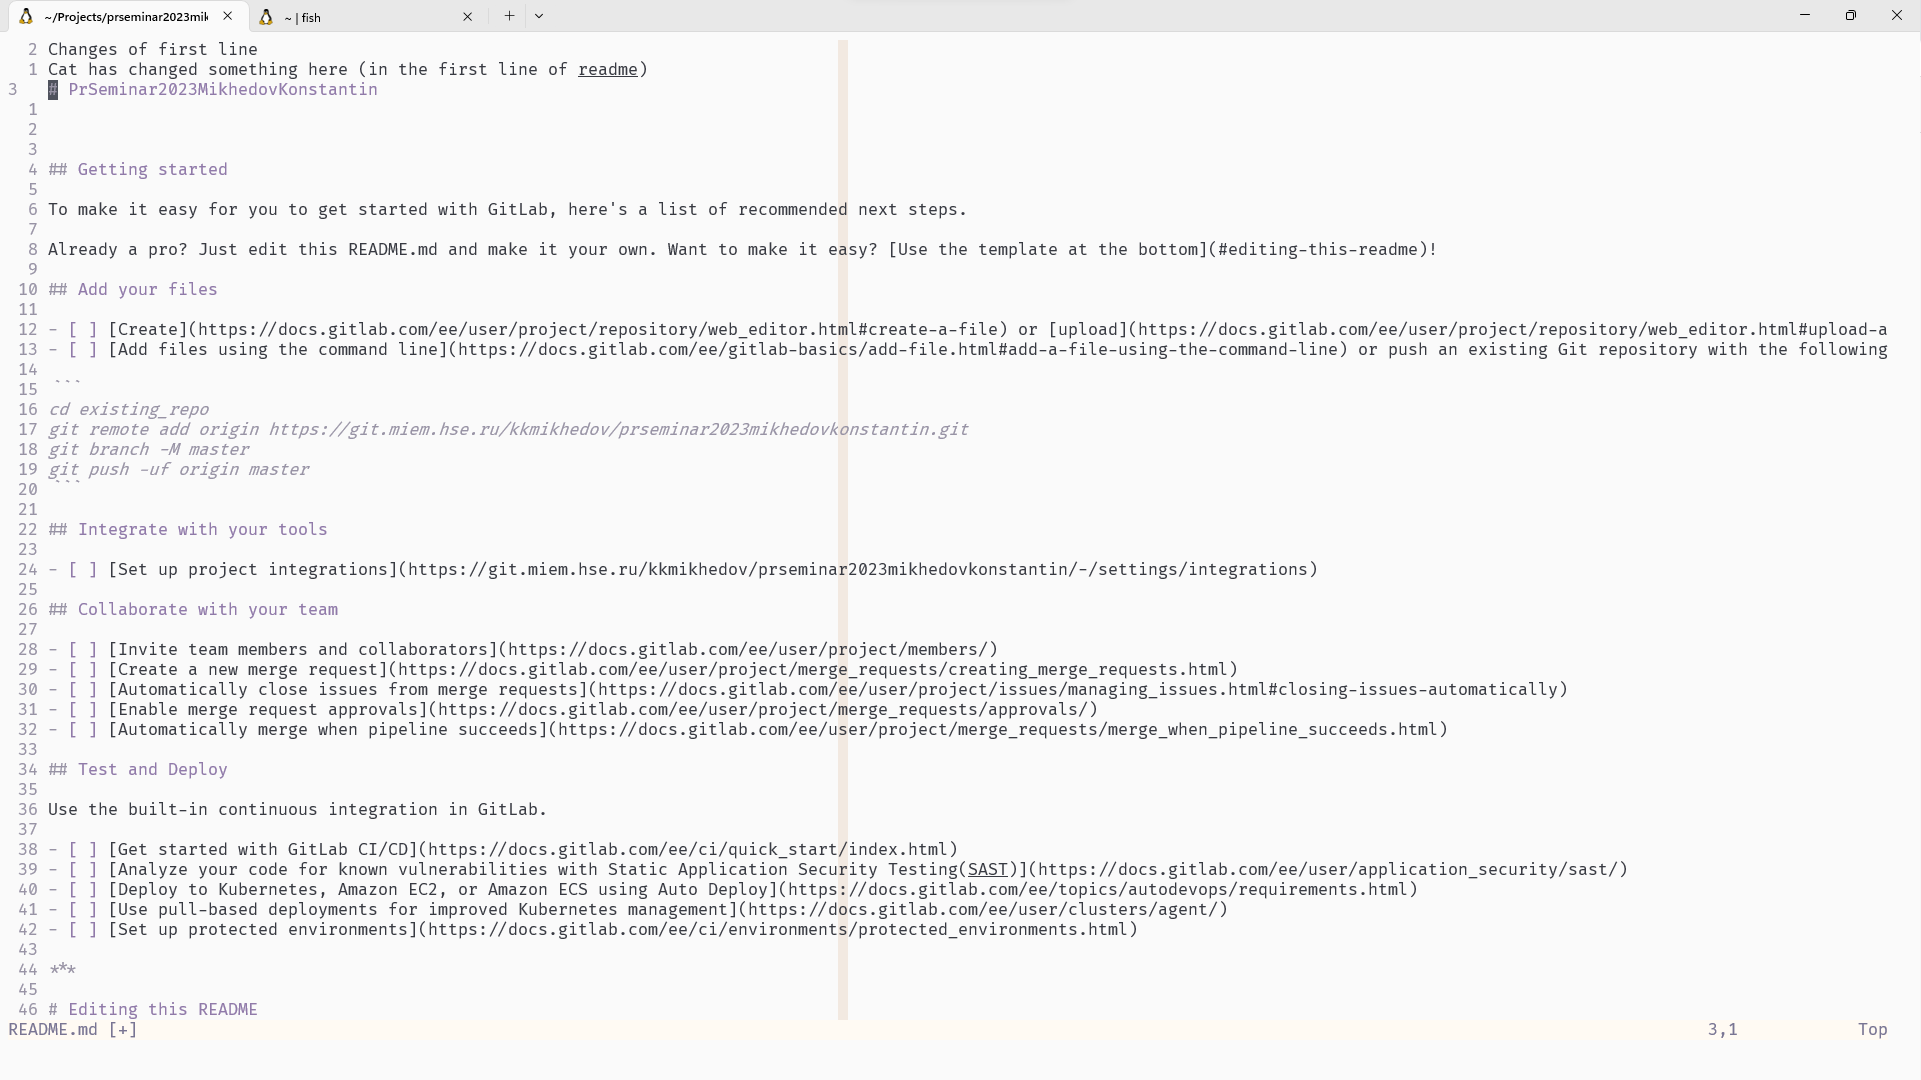
\includegraphics[width=\textwidth]{1_ (9)}
    \caption{Конфликт исчерпан, сохраняем и закрываем}
  \end{figure}

  \begin{figure}[H]
    \centering
    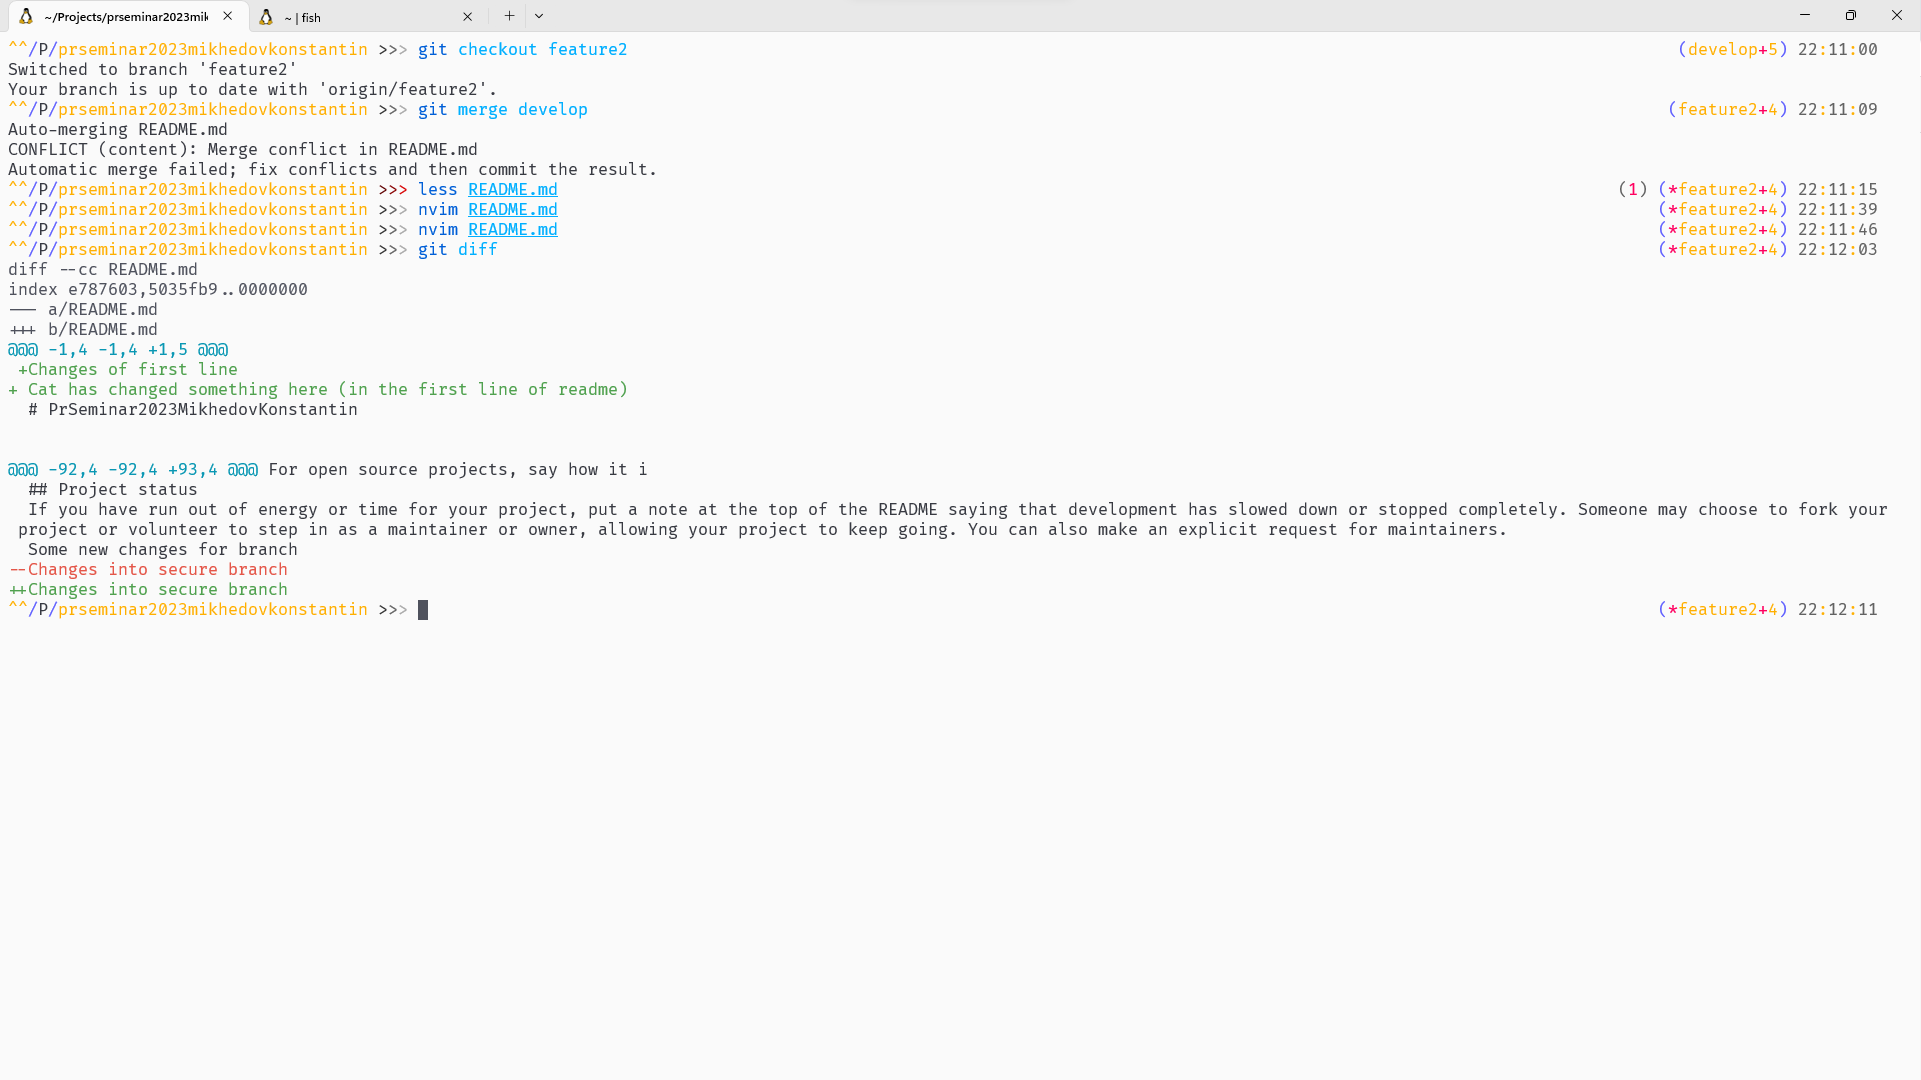
\includegraphics[width=\textwidth]{1_ (8)}
    \caption{Смотрим, что изменилось}
  \end{figure}

  \begin{figure}[H]
    \centering
    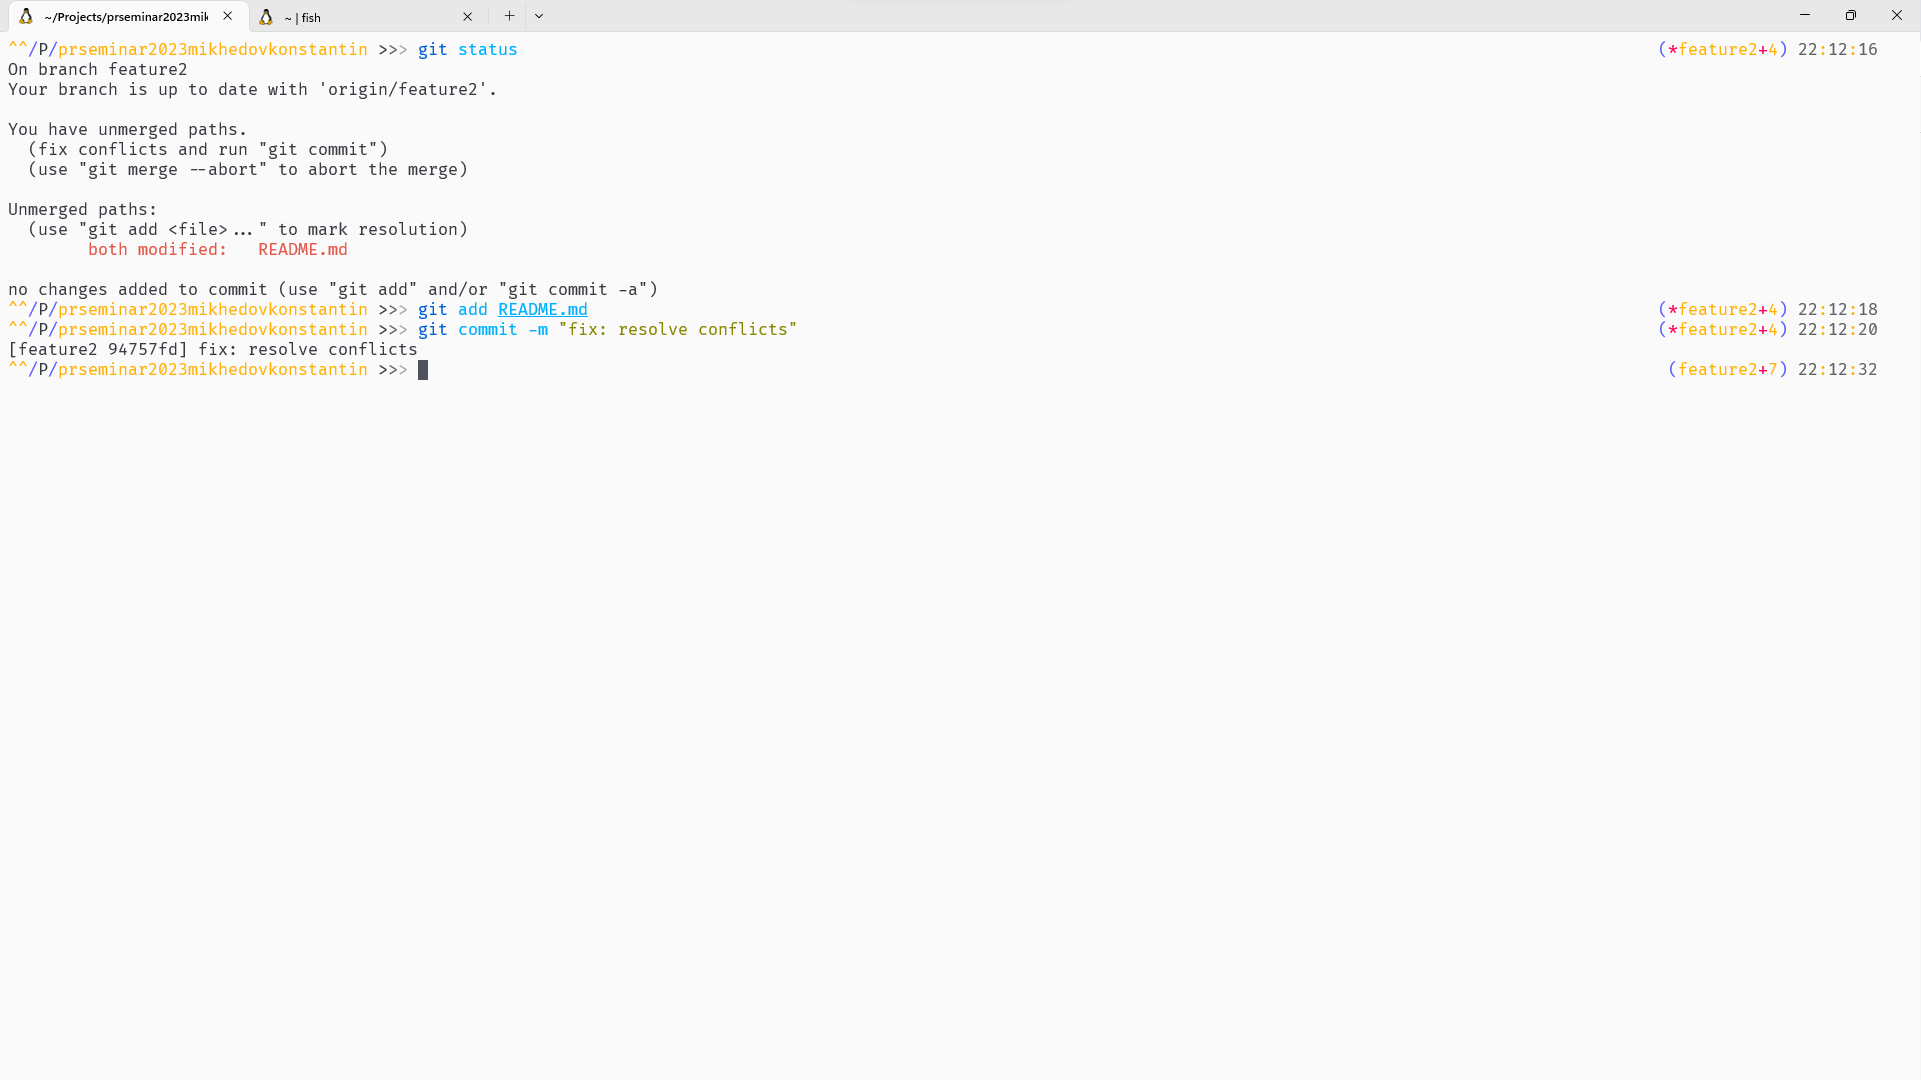
\includegraphics[width=\textwidth]{1_ (7)}
    \caption{Коммитим изменения - конфликта больше нет}
  \end{figure}

  \begin{figure}[H]
    \centering
    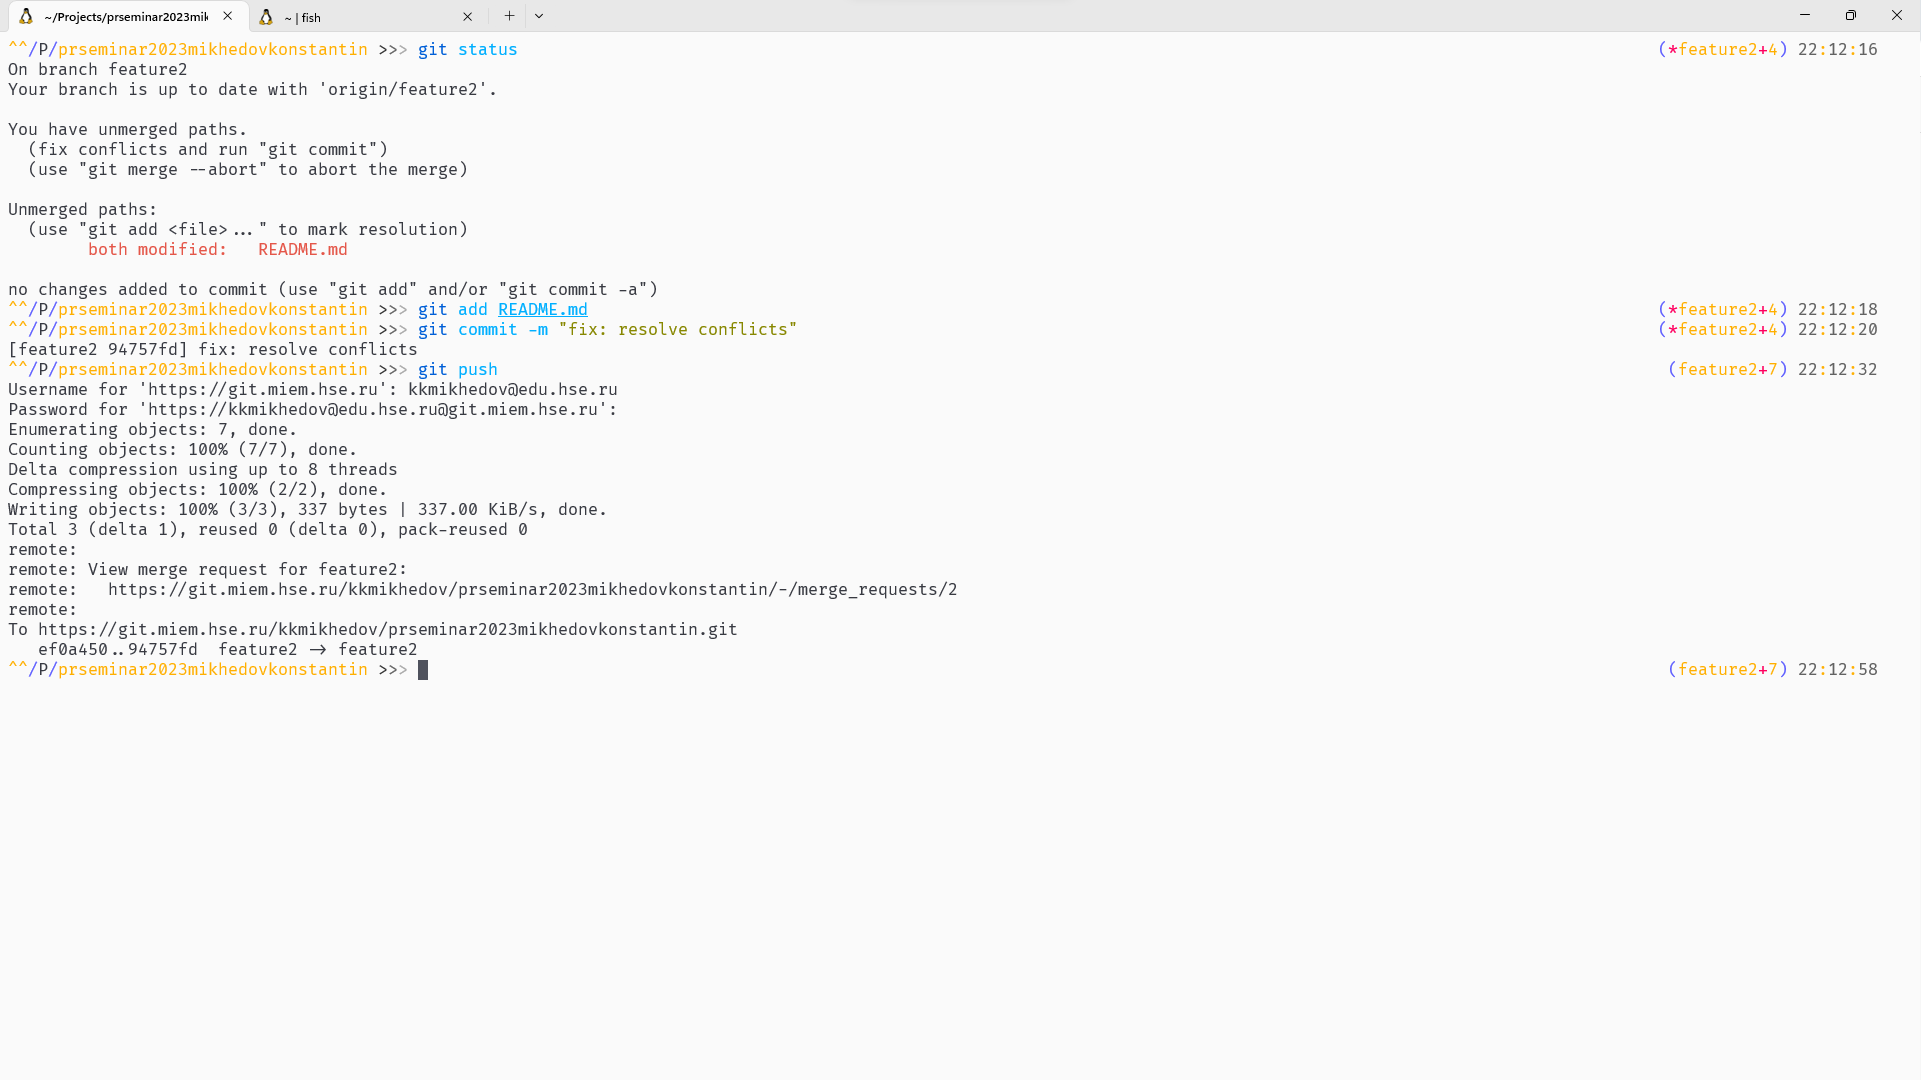
\includegraphics[width=\textwidth]{1_ (6)}
    \caption{Пушим изменения на удаленный репозиторий}
  \end{figure}

  \begin{figure}[H]
    \centering
    \includegraphics[width=\textwidth]{1_ (5)}
    \caption{Сообщение о конфликте пропало}
  \end{figure}

  \begin{figure}[H]
    \centering
    \includegraphics[width=\textwidth]{1_ (4)}
    \caption{Отключаем удаление ветки feature2 после закрытия merge request}
  \end{figure}

  \begin{figure}[H]
    \centering
    \includegraphics[width=\textwidth]{1_ (3)}
    \caption{Merge прошел успешно}
  \end{figure}

  \textbf{Ссылка на merge request (feature2 -> develop):} \href{https://git.miem.hse.ru/kkmikhedov/prseminar2023mikhedovkonstantin/-/merge_requests/2}{есть такое}

  \begin{figure}[H]
    \centering
    \includegraphics[width=\textwidth]{1_ (2)}
    \caption{Посмотрим графическое отображение веток}
  \end{figure}

  \begin{figure}[H]
    \centering
    \includegraphics[width=\textwidth]{1_ (1)}
    \caption{Выглядит все примерно так, как и должно было выглядеть}
  \end{figure}

\end{document}

